\documentclass[sigconf,review]{acmart}
\usepackage[caption=false]{subfig}
\usepackage{subcaption}

\AtBeginDocument{%
  \providecommand\BibTeX{{%
    Bib\TeX}}}
\setcopyright{acmlicensed}
\copyrightyear{2026}
\acmYear{2026}
\acmDOI{XXXXXXX.XXXXXXX}
%% These commands are for a PROCEEDINGS abstract or paper.
\acmConference[KDD '26]{The 32nd ACM SIGKDD Conference on Knowledge Discovery and Data Mining}
  {August 9--13, 2026}{Jeju, Republic of Korea}

%%
%%  Uncomment \acmBooktitle if the title of the proceedings is different
%%  from ``Proceedings of ...''!
%%
%%\acmBooktitle{Woodstock '18: ACM Symposium on Neural Gaze Detection,
%%  June 03--05, 2018, Woodstock, NY}
\acmISBN{978-1-4503-XXXX-X/2018/06}
\newtheorem{theorem}{Theorem}[section]
\newtheorem{lemma}[theorem]{Lemma}
\newtheorem{definition}[theorem]{Definition}
\newtheorem{remark}[theorem]{Remark}

\newcommand{\R}{\mathbb{R}}
\newcommand{\E}{\mathbb{E}}
\newcommand{\F}{\mathcal{F}}
\newcommand{\1}{\mathbf{1}}
\newcommand{\bphi}{\boldsymbol{\phi}}
\newcommand{\bbeta}{\boldsymbol{\beta}}
\newcommand{\bxi}{\boldsymbol{\xi}}
\newcommand{\bX}{\mathbf{X}}
\newcommand{\bL}{\mathbf{L}}
\newcommand{\bN}{\mathbf{N}}
\newcommand{\bC}{\mathbf{C}}
\newcommand{\bw}{\mathbf{w}}
\newcommand{\YS}[1]{\textcolor{red}{[YS: #1]}}


%%
%% Submission ID.
%% Use this when submitting an article to a sponsored event. You'll
%% receive a unique submission ID from the organizers
%% of the event, and this ID should be used as the parameter to this command.
%%\acmSubmissionID{123-A56-BU3}

%%
%% end of the preamble, start of the body of the document source.
\begin{document}

\title{Neural Hybrid Residual XRO Models for ENSO Forecasting}

%%
%% The "author" command and its associated commands are used to define
%% the authors and their affiliations.
%% Of note is the shared affiliation of the first two authors, and the
%% "authornote" and "authornotemark" commands
%% used to denote shared contribution to the research.
\author{Fred Xu}
\email{fredxu@cs.ucla.com}
\affiliation{%
  \institution{University of California, Los Angeles}
  \city{Los Angeles}
  \state{California}
  \country{USA}
}

\author{Kezhou Lu}
\email{melodylu@atmos.ucla.edu}
\affiliation{%
  \institution{University of California, Los Angeles}
  \city{Los Angeles}
  \state{California}
  \country{USA}
}

\author{Dmitri Kondrashov}
\email{dkondras@atmos.ucla.edu}
\affiliation{%
  \institution{University of California, Los Angeles}
  \city{Los Angeles}
  \state{California}
  \country{USA}
}


\author{Gang Chen}
\email{gchenpu@atmos.ucla.edu}
\affiliation{%
  \institution{University of California, Los Angeles}
  \city{Los Angeles}
  \state{California}
  \country{USA}
}

\author{Yizhou Sun}
\email{yzsun@cs.ucla.edu}
\affiliation{%
  \institution{University of California, Los Angeles}
  \city{Los Angeles}
  \state{California}
  \country{USA}
}

%%
%% By default, the full list of authors will be used in the page
%% headers. Often, this list is too long, and will overlap
%% other information printed in the page headers. This command allows
%% the author to define a more concise list
%% of authors' names for this purpose.
% \renewcommand{\shortauthors}{Trovato et al.}

%%
%% The abstract is a short summary of the work to be presented in the
%% article.
\begin{abstract}
We present Neural Residual Ordinary Differential Equation models for El Ni\~no-Southern Oscillation (ENSO) forecasting, combining physics-based structure with machine learning flexibility. ENSO is a primary source of seasonal predictability, and skillful ENSO forecasting delivers significant societal value. Improving forecast skill requires accurately representing ENSO's interactions with other ocean basins, but these teleconnections are complex and nonlinear. We develop a hybrid architecture that preserves the linear recharge-oscillator (RO) dynamics governing the coupled evolution of ENSO sea surface temperature and upper-ocean heat content, and employ a neural component to learn the nonlinear interactions between ENSO and other ocean basins. Our model builds on the state-of-art, physics-based Extended Recharge Oscillator (XRO), which simplifies ENSO's interactions with other ocean basins using polynomial operators. Despite only trained with scarce observational dataset, through extensive neural architecture search, we demonstrate that our architecture outperforms both the purely physics-based XRO baseline and pure deep learning models like transformers and fully non-linear neural ODEs. For deterministic forecasting, our model achieves 8.5\% reduction in RMSE over the XRO baseline while providing interpretability. For probabilistic forecasting, we introduce a two-stage stochastic training procedure with likelihood-optimized AR(1) noise, achieving 13\% improvement in Continuous Ranked Probability Score (CRPS) over XRO. Our results highlight the importance of physics-informed inductive biases for small-data climate forecasting problems and demonstrate the power of hybrid physics-neural models.
\end{abstract}

%%
%% The code below is generated by the tool at http://dl.acm.org/ccs.cfm.
%% Please copy and paste the code instead of the example below.
%%
% \begin{CCSXML}
% <ccs2012>
%  <concept>
%   <concept_id>00000000.0000000.0000000</concept_id>
%   <concept_desc>Do Not Use This Code, Generate the Correct Terms for Your Paper</concept_desc>
%   <concept_significance>500</concept_significance>
%  </concept>
%  <concept>
%   <concept_id>00000000.00000000.00000000</concept_id>
%   <concept_desc>Do Not Use This Code, Generate the Correct Terms for Your Paper</concept_desc>
%   <concept_significance>300</concept_significance>
%  </concept>
%  <concept>
%   <concept_id>00000000.00000000.00000000</concept_id>
%   <concept_desc>Do Not Use This Code, Generate the Correct Terms for Your Paper</concept_desc>
%   <concept_significance>100</concept_significance>
%  </concept>
%  <concept>
%   <concept_id>00000000.00000000.00000000</concept_id>
%   <concept_desc>Do Not Use This Code, Generate the Correct Terms for Your Paper</concept_desc>
%   <concept_significance>100</concept_significance>
%  </concept>
% </ccs2012>
% \end{CCSXML}

% \ccsdesc[500]{Do Not Use This Code~Generate the Correct Terms for Your Paper}
% \ccsdesc[300]{Do Not Use This Code~Generate the Correct Terms for Your Paper}
% \ccsdesc{Do Not Use This Code~Generate the Correct Terms for Your Paper}
% \ccsdesc[100]{Do Not Use This Code~Generate the Correct Terms for Your Paper}

%%
%% Keywords. The author(s) should pick words that accurately describe
%% the work being presented. Separate the keywords with commas.
\keywords{Climate Modeling, Neural ODE, ENSO Forecast, Time Series}
%% A "teaser" image appears between the author and affiliation
%% information and the body of the document, and typically spans the
%% page.


%% This command processes the author and affiliation and title
%% information and builds the first part of the formatted document.
\maketitle

\section{Introduction}
\label{sec:introduction}

The intersection of physics-based modeling and machine learning has emerged as a frontier for scientific prediction, particularly in domains where first-principles understanding exists but computational or modeling limitations prevent accurate forecasting. Climate science presents a compelling testbed for such hybrid approaches: while many governing physical processes are understood to the first order, comprehensive dynamical models remain imperfect, and limited observational records mean that prediction often relies on climate-model simulations rather than purely data-driven machine learning. El Ni\~no-Southern Oscillation (ENSO), the dominant mode of inter-annual climate variability~\cite{mcphaden2006enso,timmermann2018enso}, exemplifies these challenges. Despite decades of research and operational forecasting efforts, predicting ENSO beyond six months remains difficult due to chaotic dynamics, model biases, and the so-called ``spring predictability barrier''~\cite{webster1992monsoon,duan2013predictability} where forecast skill drops sharply when predictions must traverse the boreal spring season.

Traditional approaches to ENSO forecasting face many challenges. First, dynamical models based on coupled ocean-atmosphere general circulation models (GCMs)~\cite{flato2013evaluation} encode comprehensive physical processes but suffer from systematic biases, require enormous computational resources, and struggle to outperform simpler statistical methods at lead times beyond one season~\cite{barnston2012skill,Latif1998JGR, Jin2008ClimDyn}. Second, deep learning and statistical models exploit observed relationships between climate variables but typically lack interpretability and may fail when climate statistics shift---a concerning limitation given anthropogenic climate change \cite{Dmitri_model, TangangTangMonahanHsieh1998NNEOF,UbilavaHelmers2013STAR, PenlandMagorian1993LIM}.
Recent advances in deep learning have prompted efforts to apply neural networks directly to climate prediction, with notable successes in multi-year ENSO forecasting~\cite{ham2019deep, Hu2021ResCNNENSO, Yan2020TCNENSO, ZhouZhang2023GeoformerENSO, Mu2024ENSOPhyNet}, albeit so far only in hindcasts and not in real-time. However, these purely data-driven approaches face a fundamental obstacle: the observational record provides at most a few hundred independent samples for training, far fewer than the millions typically required for deep learning to excel. These models have to rely on climate model simulation data with careful choices of the datasets and modalities to use, usually resulting in formidable storage and computational resources. On top of the resource challenges, these models often lack explainability, which is highly valuable for understanding natural phenomena.

This data scarcity and lack of explainability motivate the development of hybrid physics-machine learning models that combine the interpretability and sample efficiency of physics-based approaches with the flexibility and representational power of neural networks~\cite{willard2023integrating,yin2021augmenting}. The central question we address is: \emph{How can we best integrate physical structure with learned components for climate forecasting when data is severely limited?}

We build upon the Extended Recharge Oscillator (XRO) model~\cite{zhao2024xro}, a recent physics-based framework that achieves state-of-the-art ENSO forecast skill (better than the real-time skill of International Research Institute for Climate and Society (IRI) operational models 
and comparable to the most skilful AI forecast model ~\cite{ZhouZhang2023GeoformerENSO,Ham2019DeepLearningENSO}), 
by encoding the fundamental recharge-discharge dynamics~\cite{jin1997equatorial} of the tropical Pacific coupled with seasonal modulation and polynomial nonlinearities. Our contribution is the Neural Residual Extended Recharge Oscillator (NXRO) framework, inspired by neural ODE ~\cite{chen2018neuralode,rubanova2019latent}, physics-informed machine learning~\cite{karniadakis2021physics}, and differentiable physics~\cite{um2020solver,list2022learned}. This decomposition explicitly separates dynamics into a linear physics-based component and a nonlinear correction, providing strong inductive biases that enable learning from limited data. By elucidating the mathematical formulation of the base XRO, we develop 43 model variants spanning from pure physics (XRO) to pure machine learning, enabling systematic investigation of how much physical structure is necessary and where neural flexibility provides benefit.

We demonstrate the effectiveness of our framework via both out-of-sample deterministic and stochastic forecasts. Our results on deterministic forecasts highlight the importance of both physical inductive bias and the necessity of end-to-end optimization. Interestingly, we also find that adding more data samples (through climate model simulation) does not necessarily translate to better model performance, pointing to the fundamental bias in climate model simulation against observational record for time series forecasting tasks. For stochastic forecast, we introduce a simple two-stage stochastic training procedure, which achieves 13\% improvement in Continuous Ranked Probability Score (CRPS)~\cite{hersbach2000,gneiting2007} over XRO and produces better-calibrated uncertainty estimates. 

\section{Background: ENSO Dynamics and the Extended Recharge Oscillator}
\label{sec:background}

In this section we provide background on El Ni\~no-Southern Oscillation and presents the mathematical formulation of the Extended Recharge Oscillator (XRO) model that serves as our physics-based foundation.

\subsection{ENSO Dynamics}

El Ni\~no-Southern Oscillation is a coupled ocean-atmosphere phenomenon centered in the tropical Pacific Ocean and is the leading source of global climate variability and predictability~\cite{mcphaden2006enso,timmermann2018enso}. ENSO profoundly influences global climate and weather, affecting monsoons, hurricane activity, and the frequencies of droughts and floods, with cascading impacts on ecosystem and human society worldwide. ENSO exhibits an oscillatory cycle in which sea surface temperature (SST) anomalies in the central-eastern tropical Pacific alternate between warm (El Ni\~no) and cool (La Ni\~na) phases, accompanied by changes in equatorial trade winds and a seesaw in tropical rainfall, typically recurring on approximately 2-7 year timescales. This oscillatory behavior can be interpreted using a conceptual recharge oscillator (RO) framework ~\cite{jin1997equatorial,ZebiakCane1987, Bjerknes1969Teleconnections}. When the equatorial Pacific surface warms, the trade winds weaken, which helps sustain the warming locally but also gradually redistributes upper-ocean warm water in a way that depletes equatorial upper-ocean heat content (a ``discharge''), eventually damping the warm SST anomalies. As the surface cools, the trade winds strengthen, equatorial heat content rebuilds (a ``recharge''), and conditions become favorable for the next warm phase. 

% Traditionally it has been a challenging problem in climate science to forecast ENSO at medium and long range, a problem that is challenging even for machine learning models, which are data-hungry and often rely on climate simulation data to train. However, these climate simulation data can be biased, leading to ill-calibrated predictions \cite{KimJeongJin2017SciRep, Capotondi2015ModelBiasesENSO}. 

\subsection{Cross-Basin ENSO Interactions and the Extended Recharge Oscillator (XRO) Model}

While ENSO is primarily a tropical Pacific phenomenon, numerous studies show that interactions with other ocean basins could enhance the ENSO predictions (e.g. ~\cite{zhao2024xro, cai2019pantropical}). In fact, ~\cite{zhao2024xro} augmented the traditional recharge-oscillator framework by incorporating ENSO's seasonally varying interactions with SST patterns across the different ocean basins, yielding a purely physics-based forecast model that outperforms operational climate models and achieves prediction skill comparable to state-of-the-art AI models. To describe the cross-basin ENSO interactions, \cite{zhao2024xro} leverage SST anomaly-based climate indices spanning the Indian Ocean, the North and South Pacific, the equatorial Atlantic, and the North and South Atlantic, and incorporate them into the Extended Recharge Oscillator (XRO) model to quantify both linear and nonlinear relationships. The XRO model includes a deterministic and stochastic component, each used for the corresponding forecasting task. The full model takes the form: %\YS{can we also include the concrete form? $\phi(t)$ (Fourier features) is mentioned in next session, but not list here.} \YS{it contains stochastic term. Is it fair to compare with the deterministic version mentioned in the next section?} \textcolor{blue}{XRO in fact separated the deterministic and the stochastic parts when they are doing forecast. The $\xi$ is only used when they do stochastic forecast. We compared with both the deterministic and stochastic cases, so the comparison is fair.}
\begin{align}
    \frac{d\bX}{dt} = \bL(t) \cdot \bX + \bN(\bX, t) + \sigma_\xi \bxi, \quad \frac{d\bxi}{dt} = -r_\xi \bxi + w(t), \label{eq:xro_noise}
\end{align}
\noindent where $\bX = [\bX_{\text{ENSO}}^\top, \bX_M^\top]^\top$ is the state vector consisting an ENSO component ($\bX_{\text{ENSO}}^\top$) as well as climate modes representing sea surface temperature changes in other ocean basins ($\bX_M^\top$). The ENSO component $\bX_{\text{ENSO}} = [T, h]^\top$ contains SST anomaly in equatorial Pacific ($T$) and sub-surface ocean thermocline depth anomaly representing the ocean heat content ($h$). Eight climate indices are used to construct $\bX_M^\top$. The linear operator $\bL$ captures both seasonally-varying internal recharge-discharge behavior and the cross-basin interactions between $\bX_{\text{ENSO}}$ and $\bX_M^\top$ through Fourier expansion:
\begin{equation}
    \bL(t) = \sum_{k=0}^{K} \left[ \bL_k^c \cos(k\omega t) + \bL_k^s \sin(k\omega t) \right],
    \label{eq:seasonal_L}
\end{equation}
where $\omega = 2\pi$ year$^{-1}$ is the annual frequency, $K$ is the number of harmonics retained (typically $K=2$ to capture semi-annual variations), and $\bL_k^c, \bL_k^s \in \R^{n \times n}$ are coefficient matrices. As  suggested by previous studies, ENSO exhibits amplitude-dependent behavior~\cite{an2004nonlinearity}: large El Ni\~no events decay differently than weaker events, and the warm and cold phases are asymmetric. The XRO model introduces quadratic nonlinear terms $\bN$ to capture these nonlinearities. In addition, the model includes a red-noise stochastic forcing term $\bxi(t)$ to represent unresolved atmospheric variability, such as the Madden-Julian Oscillation ~\cite{madden1971detection,zhang2005mjo} and westerly wind bursts~\cite{harrison1997westerly}, which can trigger or modify ENSO events; here $w(t)$ denotes white noise and $r_\xi$ is decorrelation time scale.

% \paragraph{Teleconnection and Climate Modes: } An interesting and challenging phenomenon to model for climate indices is that climate variability is often characterized through spatial patterns called ``modes'' that capture the dominant structures of variability in the ocean-atmosphere system. Each mode is associated with a time-varying amplitude  that quantifies how strongly the pattern is expressed at any given time. For ENSO prediction, we work with a state vector comprising indices that capture both local ENSO dynamics and remote teleconnections that influence ENSO evolution \cite{bjerknes1969atmospheric}. We follow the setup of XRO \cite{zhao2024xro} and use the following climate indices, derived from the ORAS5 ocean reanalysis\cite{zuo2019oras5}: Ni\~no3.4 Index ($T$),  Warm Water Volume ($H$) \cite{meinen2000observations}, Indian Ocean Dipole (IOD) \cite{saji1999dipole}, Southern Indian Ocean Dipole (SIOD) \cite{Jo2022SIOD_CPEN}, Indian Ocean Basin (IOB), North Pacific Meridional Mode (NPMM) \cite{chiang2002tropical}, South Pacific Meridional Mode (SPMM)  \cite{ZhangClementDiNezio2014SPMM}, Tropical North Atlantic (TNA) \cite{HamEtAl2013NTAENSOTrigger}, Atlantic 3 (ATL3) \cite{HamKugPark2013AtlanticRoles},  and South Atlantic Subtropic Dipole (SASD) \cite{HamEtAl2021SouthAtlanticENSO}. 


% \subsection{The Extended Recharge Oscillator (XRO) Model}

% A well-known physical model that captures the essential ENSO dynamics in a minimal two-variable system is the Recharge Oscillator Model \cite{jin1997equatorial}. The Extended Recharge Oscillator~\cite{zhao2024xro} generalizes it by (1) coupling ENSO with autoregressive model representations for other climate modes, (2) adding seasonal modulation of all operator parameters, and (3) including nonlinearities that capture amplitude-dependent dynamics. The XRO model dynamics for the full state vector $\bX$ takes the form:
% \begin{align}
%     \frac{d\bX}{dt} &= \bL(t) \cdot \bX + \bN(\bX, t) + \sigma_\xi \bxi \label{eq:xro_full}\\
%     \frac{d\bxi}{dt} &= -r_\xi \bxi + \bw(t) \label{eq:xro_noise}
% \end{align}
% where $\bX = [\bX_{\text{ENSO}}^\top, \bX_M^\top]^\top$ is the state vector consisting of ten variables. The ENSO component $\bX_{\text{ENSO}} = [T, h]^\top$ contains the Ni\~no3.4 sea surface temperature anomaly ($T$) and thermocline depth anomaly representing the warm water volume ($h$). The other climate modes $\bX_M = [T_{\text{NPMM}}, T_{\text{SPMM}}, T_{\text{IOB}}, T_{\text{IOD}}, T_{\text{SIOD}}, T_{\text{TNA}}, T_{\text{ATL3}}, T_{\text{SASD}}]^\top$ are SST indices that interact with ENSO. The model allows for two-way interactions between ENSO and these modes.

% \paragraph{Linear Operator:} The linear operator $\bL$ has a block structure that captures both internal dynamics and inter-mode couplings:
% \begin{equation}
%     \bL = \begin{bmatrix} \bL_{\text{ENSO}} & \bC_1 \\ \bC_2 & \bL_M \end{bmatrix}
%     \label{eq:L_structure}
% \end{equation}
% where $\bL_{\text{ENSO}}$ describes the internal ENSO recharge-discharge dynamics, $\bL_M$ represents the internal processes and interactions among other climate modes, $\bC_2$ describes the teleconnection impacts of ENSO on other modes, and $\bC_1$ describes the feedback of other modes onto ENSO. To incorporate the strong seasonal dependence of ENSO and other climate modes, the operator is parameterized through a Fourier expansion:
% \begin{equation}
%     \bL(t) = \bL_0 + \sum_{k=1}^{2} \left[ \bL_k^c \cos(k\omega t) + \bL_k^s \sin(k\omega t) \right]
%     \label{eq:seasonal_L}
% \end{equation}
% where $\omega = 2\pi/(12 \text{ months})$ is the annual frequency, and subscripts 0, 1, and 2 indicate the mean, annual cycle, and semi-annual components, respectively.

% \paragraph{Nonlinearities:} Observations and theoretical analysis indicate that ENSO exhibits amplitude-dependent behavior~\cite{an2004nonlinearity}: large El Ni\~no events decay differently than small ones, and the system shows asymmetry between warm and cold phases. XRO captures these effects through quadratic nonlinear terms. The full nonlinearity $\bN(\bX,t) = [\bN_{\text{ENSO}}^\top, \bN_M^\top]^\top$ consists of ENSO nonlinearities:
% \begin{equation}
%     \bN_{\text{ENSO}} = \begin{bmatrix} b_1 T^2 + b_2 T h \\ 0 \end{bmatrix}
%     \label{eq:N_enso}
% \end{equation}
% These can be related to deterministic nonlinear ocean advection as well as atmospheric nonlinearity through the nonlinear SST-wind stress feedback. A local quadratic nonlinearity is also incorporated for the Indian Ocean Dipole to capture its observed asymmetry:
% \begin{equation}
%     \bN_M = [0, 0, 0, b_3 T_{\text{IOD}}^2, 0, 0, 0, 0]^\top
%     \label{eq:N_iod}
% \end{equation}
% The nonlinear terms for modes other than IOD are set to zero given their smaller observed asymmetry and skewness. Like the linear operator, the nonlinear coefficients are seasonally modulated via Fourier expansion.

% \paragraph{Stochastic Forcing:} The term $\bxi(t)$ represents stochastic forcing from unresolved atmospheric variability, particularly the Madden-Julian Oscillation~\cite{madden1971detection,zhang2005mjo} and westerly wind bursts~\cite{harrison1997westerly} that can trigger or modify ENSO events. This forcing is modeled as red noise with decorrelation time scales $r_\xi$ and amplitudes $\sigma_\xi$. In equation~\eqref{eq:xro_noise}, $\bw(t)$ denotes white noise with a Gaussian distribution $\mathcal{N}(0, r_\xi^2)$, ensuring that the variance of $\bxi$ is maintained at unit level.

\subsection{Limitations Motivating Neural Extensions}

While XRO achieves strong forecast skill and provides physically interpretable parameters, several limitations motivate the development of neural-augmented variants: 

\begin{enumerate}
    \item \textbf{Representation:} The quadratic nonlinearities assume specific functional forms derived from physical intuition. If the true dynamics contain nonlinearities outside this prescribed form, XRO cannot capture them.
    \item \textbf{Optimization:} XRO parameters are estimated using multivariate linear regression with a forward-differencing scheme. This optimizes one-step prediction error for each equation. During multi-step forecasting, however, all variables evolve together in a coupled system where errors propagate and compound.
\end{enumerate}


\section{Neural Residual Dynamics}
\label{sec:neural_ode}

The limitations of XRO identified in Section~\ref{sec:background} motivate a neural extension that preserves the model's physical interpretability while adding flexibility. In this section, we develop the Neural Residual ODE framework, decomposing the dynamics into a linear component inspired by physical model and a nonlinear residual correction.

\subsection{Motivation: Physics-Informed Residual Learning}

The central insight of our approach is that the XRO linear operator captures the dominant, well-understood physics of ENSO: the recharge-discharge mechanism, seasonal modulation of coupling strengths, and teleconnections among climate modes, which generalizes robustly across climate regimes \cite{zhao2024xro}. However, the polynomial nonlinearities in XRO impose strong assumptions about functional form that may not match the true dynamics and can lead to overfitting. In addition, the linear and non-linear term can be optimized end-to-end for better coupling.

Rather than specifying the nonlinear dynamics apriori, we propose to \emph{learn} them from data through a neural network that captures the residual between the linear physics model and observations. Recent works have demonstrated the effectiveness of this paradigm across scientific machine learning~\cite{karniadakis2021physics,willard2023integrating}, including learning corrections to fluid simulations~\cite{um2020solver,list2022learned}, augmenting physical models for complex dynamics forecasting~\cite{yin2021augmenting}, and discovering missing physics in partial differential equations~\cite{raissi2019pinn}. The key is to let the physics-based component handle what it does well (linear dynamics, seasonal structure) while delegating the remainder to a flexible function approximator that can adapt to the specific dataset. This explicit linear-plus-nonlinear decomposition offers several advantages. First, the linear operator provides strong inductive bias that reduces the effective hypothesis space, enabling learning from limited data, a critical consideration when training samples number in the hundreds rather than millions. Second, the neural residual needs only capture the \emph{difference} between true dynamics and the linear approximation, a smaller signal that is easier to learn than the full dynamics. Third, the approach naturally controls the contribution of nonlinear component, balancing both effects.

\subsection{Model Formulation}

We model the evolution of the climate state vector $\bX(t) \in \R^n$ as a continuous-time dynamical system, inspired by neural ODE methods~\cite{chen2018neuralode, huang2023generalizinggraphodelearning}:
\begin{equation}
    \frac{d\bX}{dt} = \bL_\theta(t) \cdot \bX + R_\phi([\bX, \bphi(t)]),
    \label{eq:nxro_main}
\end{equation}
where $\bL_\theta(t) \in \R^{n \times n}$ is a seasonally-modulated linear operator with learnable parameters $\theta$, following the form in Equation \ref{eq:seasonal_L}. $R_\phi$ is a neural network residual, and $\bphi(t)$ encodes seasonal context through Fourier features. The linear operator inherits the Fourier structure from XRO, expanded to the second harmonic to capture semi-annual variations. This parameterization ensures that the linear dynamics vary smoothly with season, capturing the well-documented seasonal dependence of ENSO growth rates and teleconnection strengths.
\paragraph{Seasonal Context Features:} To provide the residual network with information about the current season, we construct Fourier features encoding the annual cycle:
\begin{equation}
    \bphi(t) = [1, \cos(\omega t), \sin(\omega t), \cos(2\omega t), \sin(2\omega t)]^\top \in \R^5
\end{equation}
These features allow the residual to learn seasonally-varying corrections. The constant term enables the network to learn season-independent corrections, while the harmonic terms capture annual and semi-annual modulation.

\paragraph{Neural Residual Network:} The residual function $R_\phi$ is parameterized by default as a MLP that take the concatenation of the state vector and seasonal features as input.  The MLP architecture is deliberately simple, with 3-layers and hidden dimension of 64. Since we are extending the XRO model with neural components, we call the resulting model Neural Extended Recharge Oscillator (NXRO). Note that our proposed neural residual model can potentially be applied to other scientific domains, and in this project we only focus on the task of ENSO forecasting.

\paragraph{Training Procedure:} We train the model end-to-end by minimizing the mean squared forecast error across multiple lead times. Let $\{(\bX_i^{\text{obs}}, t_i)\}_{i=1}^N$ denote the training observations, where $\bX_i^{\text{obs}}$ is the observed state at time $t_i$. For each initialization time $t_i$, we integrate the model forward to generate forecasts $\hat{\bX}_i(t_i + \ell)$ at leads $\ell = 1, \ldots, L_{\max}$ months. The training objective is:
\begin{equation}
    \mathcal{L}(\theta, \phi) = \frac{1}{N \cdot L_{\max}} \sum_{i=1}^{N} \sum_{\ell=1}^{L_{\max}} \left\| \hat{\bX}_i(t_i + \ell) - \bX_i^{\text{obs}}(t_i + \ell) \right\|^2
    \label{eq:loss}
\end{equation}
where $L_{\max} = 21$ months in our experiments, covering the operationally-relevant forecast horizon for ENSO. 
By optimizing over extended forecast trajectories, our loss rewards coefficient configurations that maintain accuracy over long integration periods.

\subsection{Alternative Nonlinear Components}
\label{sec:ablations}

While the MLP residual represents our primary model, we conduct extensive architectural search and investigate alternative parameterizations of the nonlinear component to understand which architectural choices are essential for performance. These alternatives share the same linear operator structure but differ in how they model the residual / correction term.

\subsubsection{Graph-Based Corrections}

Climate dynamics exhibit structured interactions among variables---for instance, the equatorial SST anomaly is strongly coupled to warm water volume but only weakly coupled to the Indian Ocean Dipole. A Graph Neural Network (GNN) ~\cite{kipf2017gcn,wu2020comprehensive} can encode these interaction patterns explicitly through a sparse adjacency matrix, whose entries can encode the strength of pairwise interaction. Recent works on multivariate time series forecasting with graph neural ODEs~\cite{huang2023generalizinggraphodelearning} has demonstrated the effectiveness of combining continuous-time dynamics with structured variable interactions. In particular, we consider a 2-layer Graph Convolutional Network (GCN) residual of the form: %\YS{which GNN are you using? GCN? How many layers? specify the exact form. What is the $\mathcal{E}$ in eq. 5? }
\begin{align}\label{eq:nxro_graph}
    & \frac{dX}{dt} = L_\theta(t) \cdot X + \alpha(t) \cdot \mathrm{softmax}\!\Big(\hat{A}\,\sigma\!\big(\hat{A}XW^{(0)}\big)\,W^{(1)}\Big), %\text{GCN}_\theta(X, A),
\end{align}
where in our setup, the normalized adjacency matrix $\tilde{A}$ is initialized via top-2 pairwise correlation between the historical time series at training split, while the graph nodes are each individual climate indices. The adjacency matrix is formulated as a learnable component and optimized end-to-end during model training. $\alpha(t)$ are learnable seasonal gate variables, modulating the effect of the nonlinear interaction term on the overall dynamics at different months:
\begin{equation}\label{eq:gate}
    \alpha(t) = \sigma \left( \mathbf{w}_0 + \sum_{k=1}^{K}w_{2k-1}\cos(k\omega t)+w_{2k}\sin(k\omega t) \right),
\end{equation}
where $\mathbf{w}_0,\mathbf{w}_1$ are learnable, $\sigma$ is the sigmoid activation, $\omega = 2\pi$, and $K = 2$ to capture annual and semi-annual harmonics. The graph structure provides a physics-informed sparsity pattern that prevents the model from learning spurious correlations, and the learnable seasonal gate $\alpha(t)$ captures the magnitude of GNN's influence on the overall model prediction. We call the NXRO model with GNN residual NXRO-GNN.

\subsubsection{Attention-Based Corrections}

The attention mechanism~\cite{vaswani2017attention} offers an alternative approach to modeling variable interactions, where the coupling strength depends on the current state. We implement a masked self-attention residual: %\YS{be consistent with Eq 5. write down the full ODE or just residual term.}
\begin{equation}
    \frac{d\mathbf{X}}{dt} = L_\theta(t)\cdot X + \alpha(t)\cdot \text{Proj}\left(\text{Softmax}\left(\mathbf{M} \odot \frac{\mathbf{Q}\mathbf{K}^\top}{\sqrt{d}}\right)\,\mathbf{V}\right)
\end{equation}
where $Q = \bX W_Q$, $K = \bX W_K$, $V = \bX W_V$ are learnable query, key, and value projections, $\mathbf{M}$ is a fixed masking matrix that forces sparsity, by default allowing self attention each index and attention to the two ocean indices of ENSO and WWV, following the design in \cite{zhao2024xro}, and $\alpha(t)$ provides seasonal gating in Equation \ref{eq:gate}. We call the model with Attention residual as NXRO-Attentive. % \YS{explain $W_o$. How does mask M parameterized? which part is learnable?}


\section{Experimental Evaluation: Deterministic Forecasting}
\label{sec:deterministic}

In this section, we present the results on deterministic out-of-sample forecast. We are interested in particularly the following questions:
(1) Do neural residual models outperform  purely nonlinear neural models and purely physical model? (2) Does more synthetic data from climate model simulations benefit the prediction performance?

\subsection{Experimental Setup}
\paragraph{Climate Indices and Dataset:} The ENSO indices include sea surface temperature anomalies averaged over Ni\~no 3.4 region 170$^\circ$-120$^\circ$W, 5$^\circ S$-5$^\circ$N (T) and the depth of the 20 $^\circ C$ subsurface isotherm averaged over the equatorial Pacific 120$^\circ$E-80$^\circ$W, 5$^\circ S$-5$^\circ$N (h). The non-ENSO climate-modes climate modes in other ocean basins (i.e., $\bX_M^\top$) are defined based on area-weighted means of sea surface temperature anomalies: three in the Indian Ocean, two in the Pacific (North/South), and three in the Atlantic (North/South/equatorial) (Appendix B). For observational dataset, we utilize the SST and three-dimensional subsurface ocean temperature produced by ECMWF Ocean Reanalysis System 5 (ORAS5), ranging from 1958-2023 \cite{zuo2019oras5}. The training period spans January 1979 through December 2001, comprising 276 monthly observations over 23 years. The test period spans January 2002 through December 2022, comprising 252 monthly observations over 21 years. We evaluate ENSO forecasts at lead times from 1 to 21 months, covering the operationally-relevant horizon for ENSO prediction. In the transfer-learning experiment, we use $100$ members of large ensemble historical simulations from Community Earth System Model, version 2 (CESM) \cite{LENS}. For each CESM ensemble member, we extract the same set of climate indices and temporal ranges as in the observation data.

\paragraph{Evaluation Metrics:} We use root mean squared error (RMSE) to measure the typical magnitude of forecast errors in degrees Celsius, with lower values indicating better performance, and anomaly correlation coefficient (ACC), which measures the linear association between forecasts and observations. These two metrics are standard for evaluating deterministic ENSO forecast \cite{zhao2024xro, TangangTangMonahanHsieh1998NNEOF, KondrashovKravtsovRobertsonGhil2005EMR}. 

\paragraph{Baselines:}To better understand the first question above, we include models that are purely neural (fully-nonlinear Neural ODE \cite{chen2018neuralode}, transformer \cite{vaswani2017attention}), purely physical (XRO \cite{zhao2024xro}), and a large number of neural residual models, including NXRO-MLP, NXRO-Graph, NXRO-Attentive, and $35$ others, covering extensive neural architectural search (full list in Appendix \ref{app:a1}). The baseline Neural ODE model takes the generic form as in ~\cite{chen2018neuralode}, which parametrizes the entire vector field  as a 3-layer MLP. As for the transformer model, we use the tokenization approach from models like Informer  \cite{zhou2021informerefficienttransformerlong} and Autoformer \cite{wu2022autoformerdecompositiontransformersautocorrelation}, which tokenizes the time series variables alongside the time stamps, encoding month-of-year and providing  periodic information. These models vary significantly on their parameter counts, with NXRO-GCN and NXRO-Attention model taking $\sim 260$ times fewer parameters than the transformer baseline. We provide  hyperparameter details in Appendix \ref{app:a1}.  


\subsection{Training Strategy and Data Source}
 
To study the second question, we examine whether pre-training on related datasets can improve generalization~\cite{pan2010transfer,weiss2016survey, pmlr-v202-nguyen23a, bodnar2025earthsystemfm} and investigate a two-stage training procedure: In the first stage, we train the model on synthetic climate indices derived from CESM  climate model simulations. The goal is to learn general features of climate variability that transfer to the real system. In the second stage, we fine-tune the pre-trained model on the observational data \cite{zuo2019oras5}. The pre-trained weights provide an initialization that may be closer to good solutions than random initialization, potentially enabling faster convergence and better generalization. 

\subsection{Overall Performance Comparison}

% \begin{table}[t]
\centering
\label{tab:rmse_selected_leads}
\setlength{\tabcolsep}{3.5pt} % tighten column spacing
\renewcommand{\arraystretch}{1.15}
\begin{tabular}{rcccccc}
\toprule
Lead & XRO & \shortstack{NXRO\\Attn} & \shortstack{NXRO\\GNN} & \shortstack{NXRO\\MLP} & \shortstack{Neural\\ODE} & \shortstack{Trans\\former} \\
\midrule
3  & 0.350 & 0.289 & 0.298 & \textbf{0.275} & 0.401 & 0.406 \\
6  & 0.558 & 0.456 & 0.479 & \textbf{0.440} & 0.628 & 0.622 \\
9  & 0.659 & 0.571 & 0.598 & \textbf{0.571} & 0.718 & 0.749 \\
12 & 0.704 & \textbf{0.659} & 0.682 & 0.672 & 0.786 & 0.858 \\
15 & 0.763 & \textbf{0.740} & 0.750 & 0.778 & 0.859 & 0.948 \\
18 & 0.809 & 0.787 & \textbf{0.785} & 0.851 & 0.872 & 0.987 \\
21 & 0.833 & 0.807 & \textbf{0.801} & 0.883 & 0.856 & 0.968 \\
\midrule
Parameters & 650 & 633 & 537 & 6334 & 5514 & $\sim$ 170K \\ 
\bottomrule
\end{tabular}
\caption{RMSE at selected lead times  for the models explored in Figure \ref{fig:1c_core_models_ranking}. Best (lowest) RMSE per row is in bold. We see a clear pattern that MLP based nonlinear component performs the best at short-term, while attention starts to pick up at medium-term, and GNN at long-term. Overall all the NXRO variants consistently outperform the XRO baseline and the purely non-physical models.}
\end{table}

\begin{figure}
    \centering
    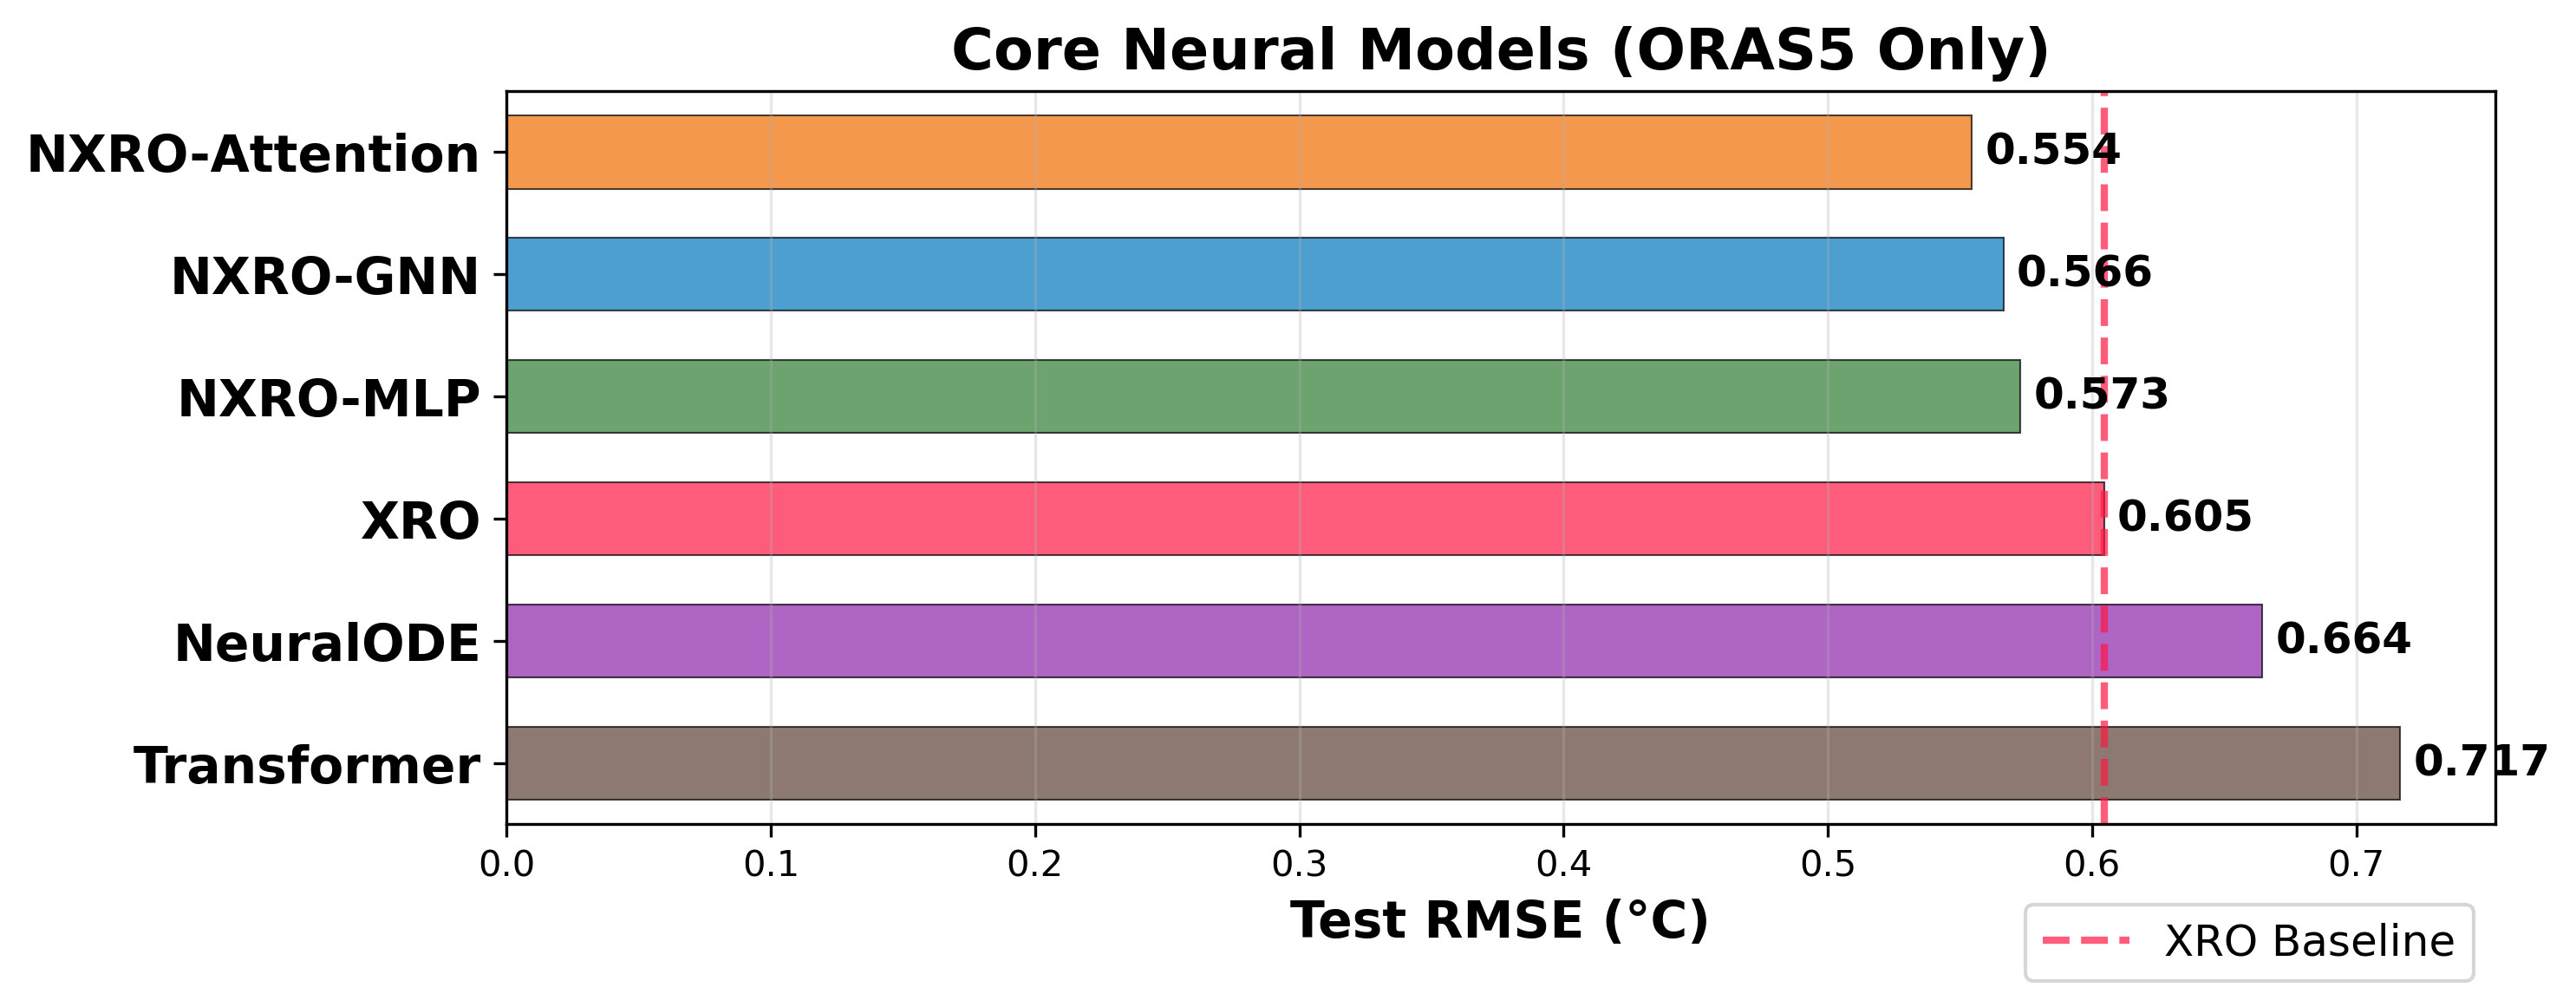
\includegraphics[width=\columnwidth]{figures/1c_core_models_ranking.png}
    \caption{Average RMSE across 21 lead times on the out-of-distribution ENSO forecast. NXRO variants outperform baselines by a significant margin.}
    \label{fig:1c_core_models_ranking}
\end{figure}
\begin{table}[t]
\centering
\setlength{\tabcolsep}{3.5pt} % tighten column spacing
\renewcommand{\arraystretch}{1.15}
\begin{tabular}{rccc@{\hspace{6pt}\vrule\hspace{6pt}}cccc}
\toprule
Lead & \shortstack{Neural\\ODE} & \shortstack{Trans\\former} & XRO & \shortstack{NXRO-\\MLP} & \shortstack{NXRO-\\Attn} & \shortstack{NXRO-\\GNN} \\
\midrule
3  & 0.401 & 0.406 & 0.350 & \textbf{0.275} & 0.289 & 0.298 \\
6  & 0.628 & 0.622 & 0.558 & \textbf{0.440} & 0.456 & 0.479 \\
9  & 0.718 & 0.749 & 0.659 & \textbf{0.571} & 0.571 & 0.598 \\
12 & 0.786 & 0.858 & 0.704 & 0.672 & \textbf{0.659} & 0.682 \\
15 & 0.859 & 0.948 & 0.763 & 0.778 & \textbf{0.740} & 0.750 \\
18 & 0.872 & 0.987 & 0.809 & 0.851 & 0.787 & \textbf{0.785} \\
21 & 0.856 & 0.968 & 0.833 & 0.883 & 0.807 & \textbf{0.801} \\
\midrule
Parameters & 5514 & $\sim$ 170K & 650 & 6334 & 633 & 537 \\
\bottomrule
\end{tabular}
\caption{RMSE at selected lead times  for the models explored in Figure \ref{fig:1c_core_models_ranking}. Best (lowest) RMSE per row is in bold. We see a clear pattern that MLP based nonlinear component performs the best at short-term, while attention starts to pick up at middle-term, and GNN at long-term.}
\label{tab:rmse_selected}
\end{table}

\begin{figure}
    \centering
    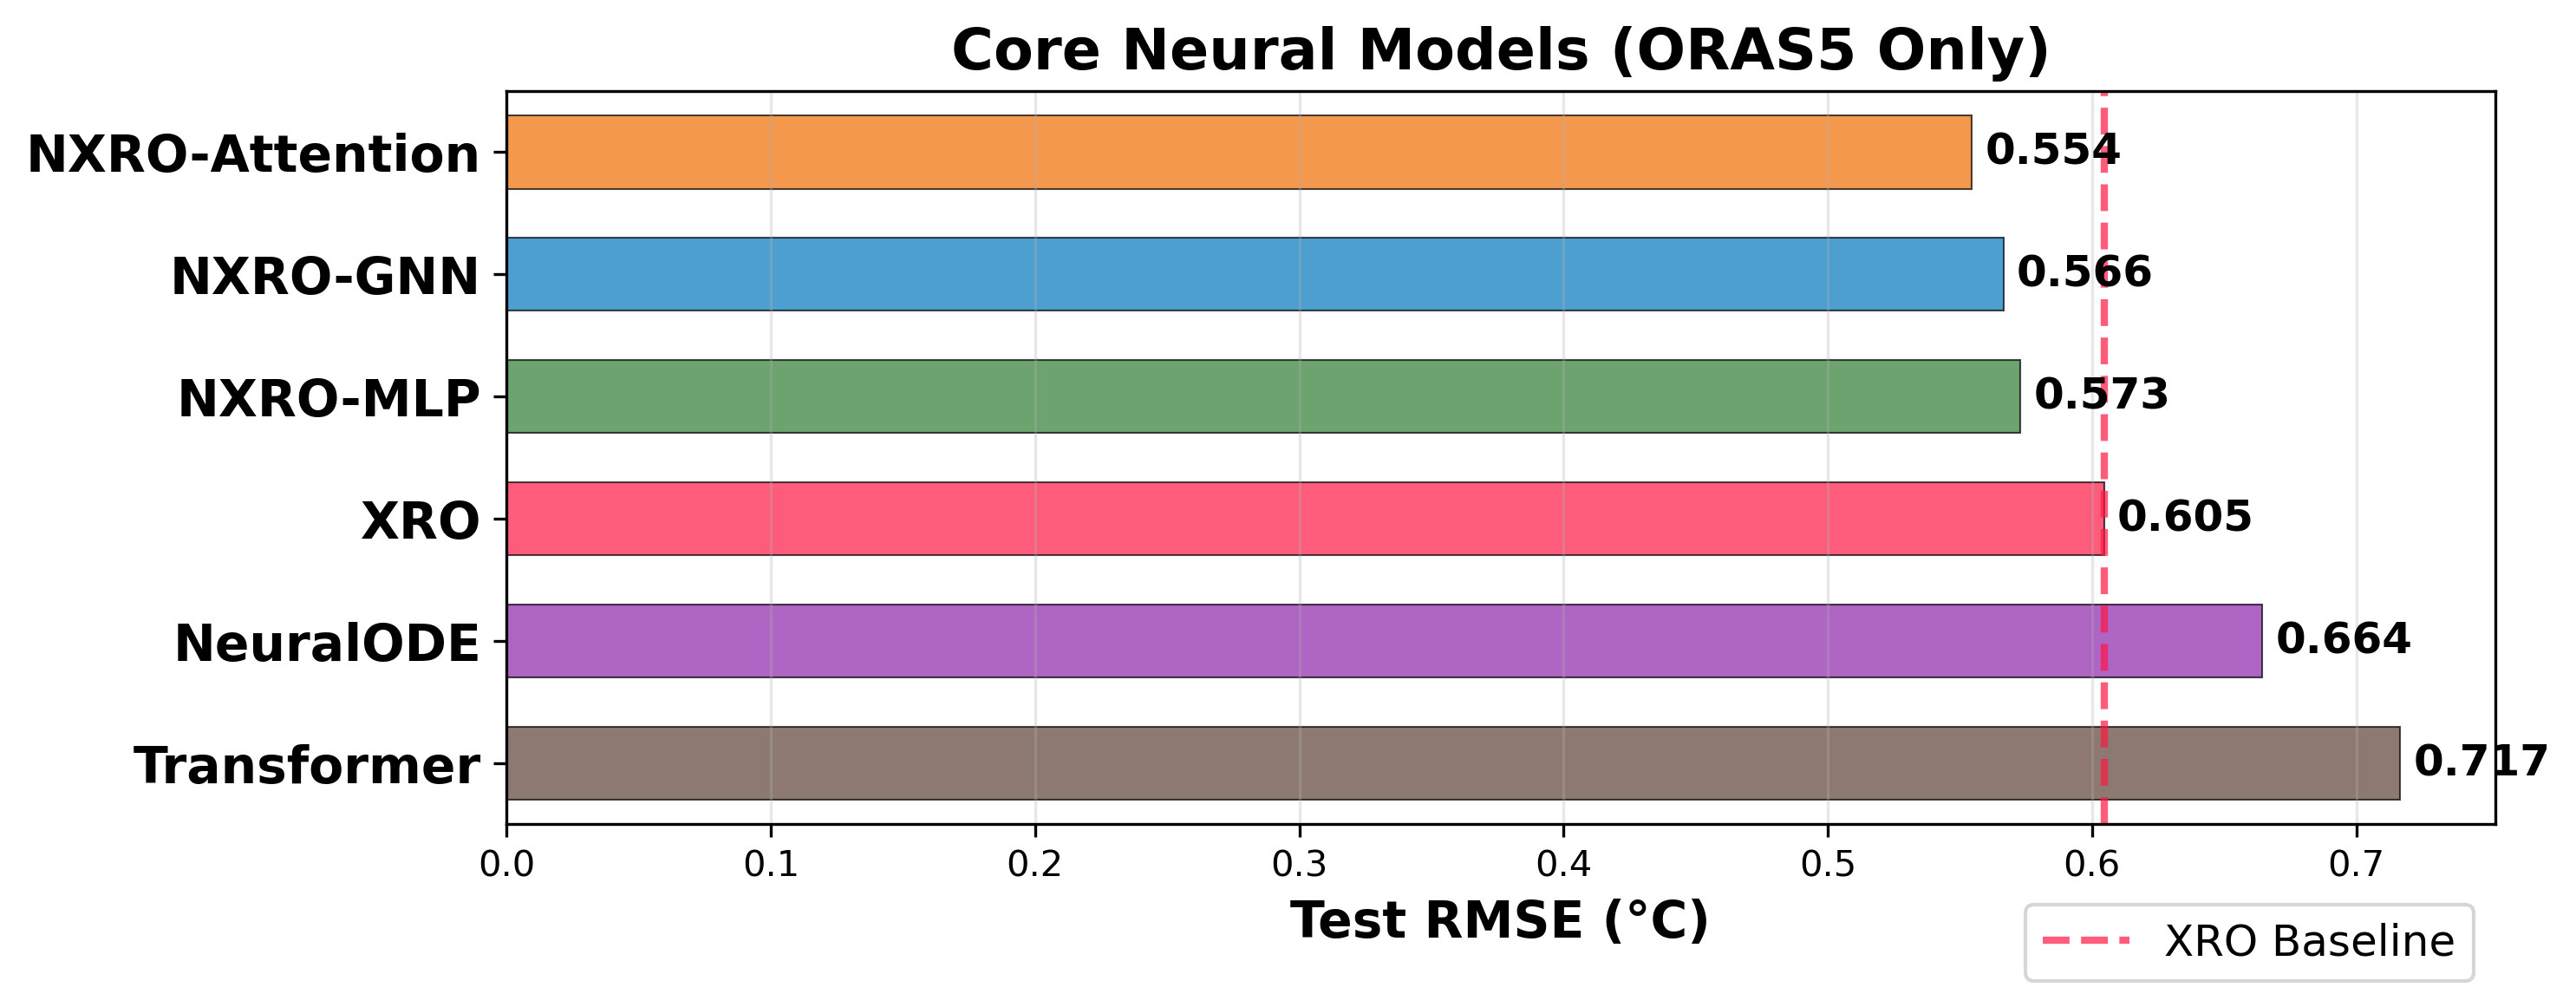
\includegraphics[width=\columnwidth]{figures/1c_core_models_ranking.png}
    \caption{Average RMSE across 21 lead times on the out-of-distribution ENSO forecast. NXRO variants outperform baselines by a significant margin.}
    \label{fig:1c_core_models_ranking}
\end{figure}

Figure \ref{fig:1c_core_models_ranking} presents the average predictive performance of the NXRO-variants, the physical XRO model, a fully nonlinear Neural ODE model, and a transformer model. The attention based neural model (NXRO-Attention) achieves the best average out-of-sample performance, with an average test RMSE of 0.554°C. This represents a 8.4\% improvement in RMSE to the XRO baseline. All variants of nonlinearity presented in Section 3 outperform the XRO baseline. Notably, the purely neural transformer model overfits severely to the small dataset, resulting in poor prediction performance. For more granular comparisons at the temporal scale, we also provide in Table \ref{tab:rmse_selected} the test RMSE at lead times $3,6,\cdots 21$ months, where a clear pattern emerges that the NXRO-MLP model variant outperforms at short lead time, but NXRO-Attention excels at medium lead time, and ultimately NXRO-GNN model dominiates at longer lead times.


Figure~\ref{fig:top10_rmse} shows the most granular comparison between the models by displaying RMSE as a function of forecast lead time for the top models: notably, the Graph based residual model  performs consistently better than the XRO model at all lead times, and the pattern from Table \ref{tab:rmse_selected} persists.  These results demonstrate that the neural ODE based residual models (NXRO variants) outperform the base XRO model in different ways and validate their effectiveness for ENSO forecast, highlighting the importance of a neural correction term. Moreover, the poor performance of the fully nonlinear neural ODE and the transformer model signals the importance of the linear component and its associated physical prior. We provide comprehensive results for all the model variants we have experimented on in Appendix A. 

\begin{figure*}[htbp]
    \centering
    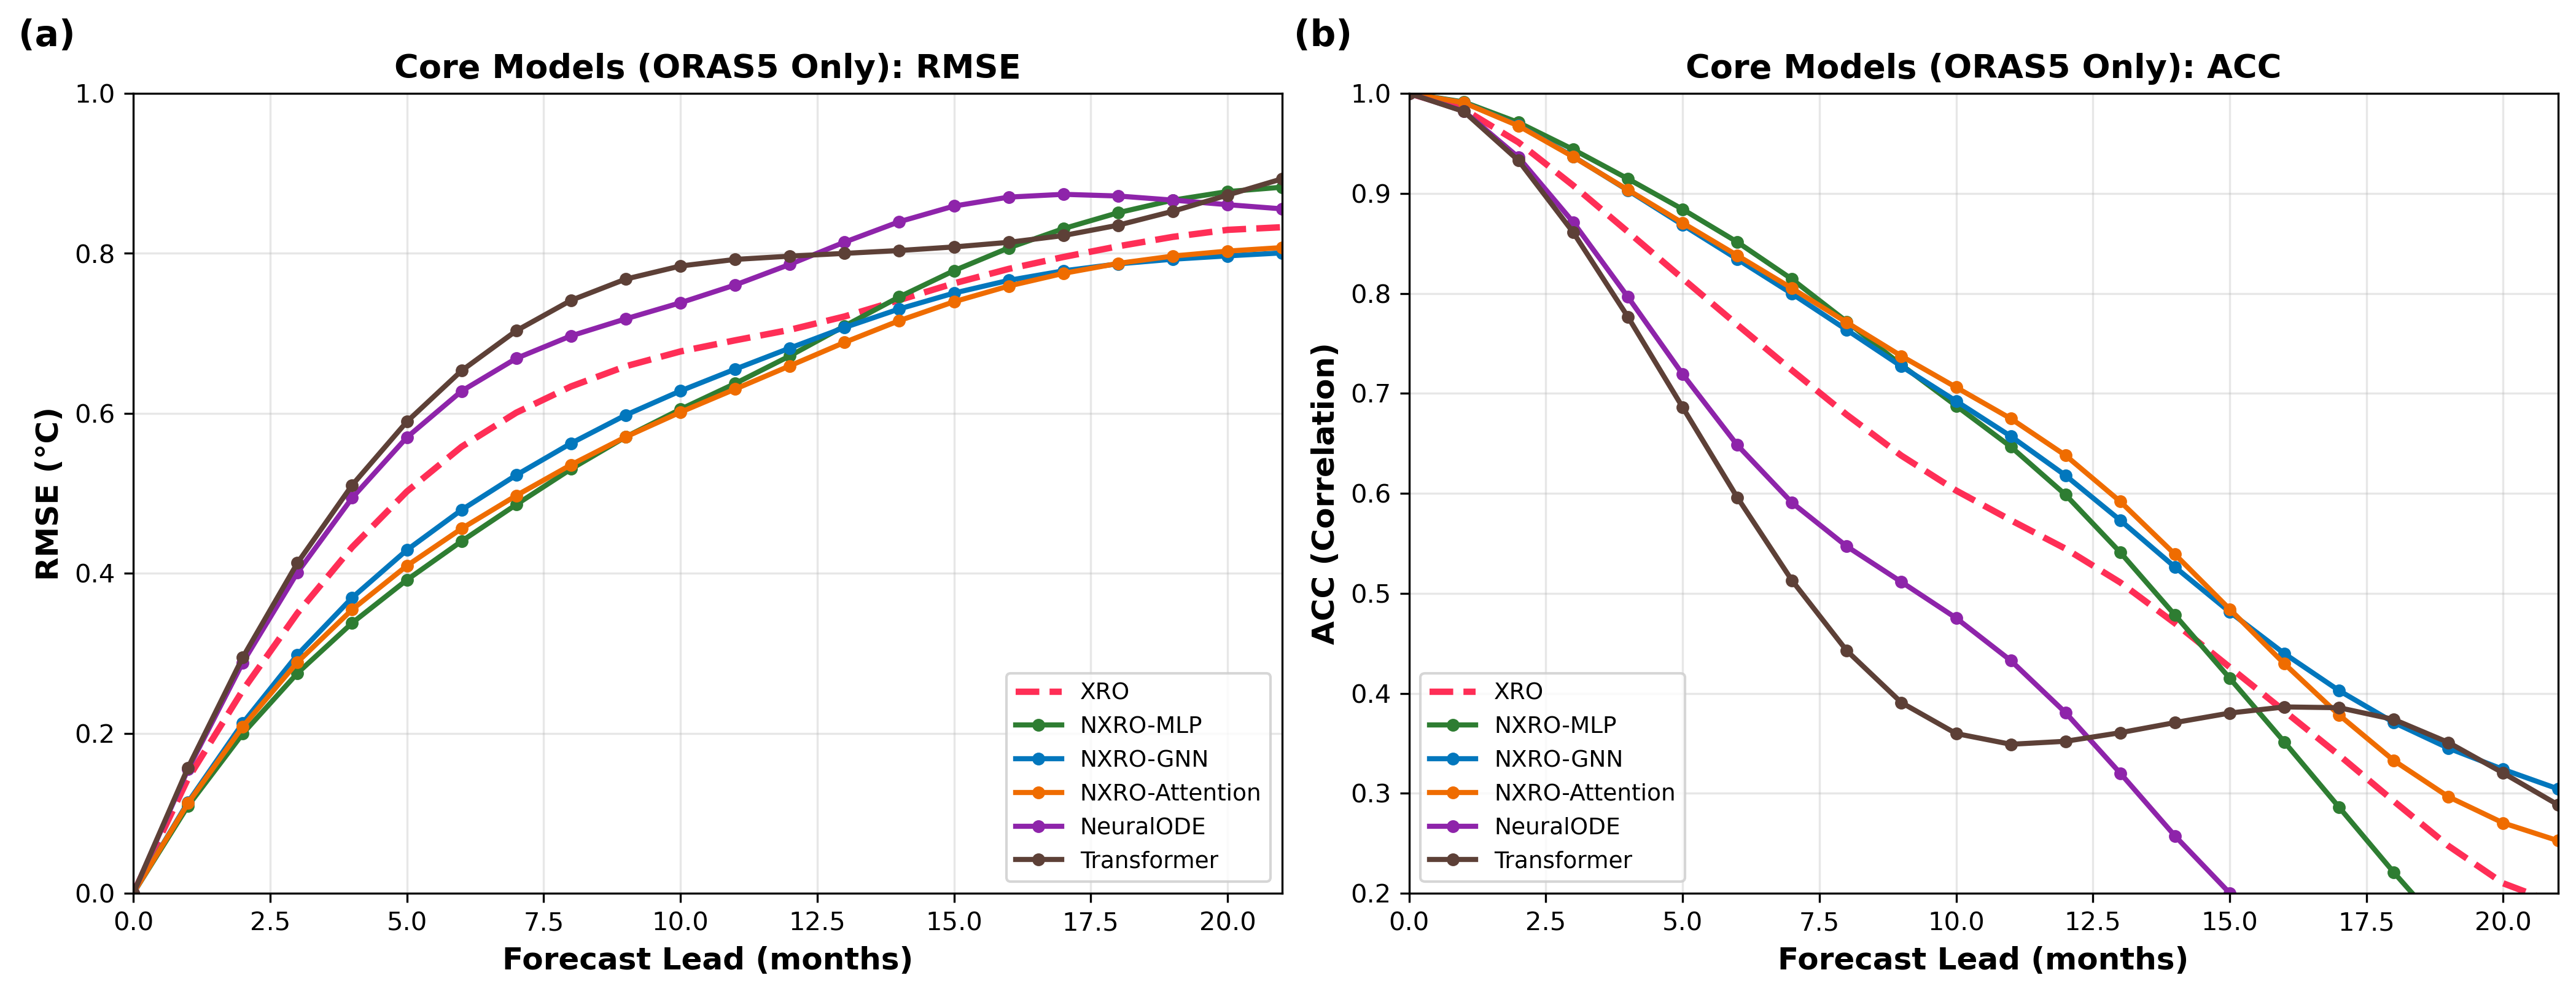
\includegraphics[width=\textwidth]{figures/1f_core_models_combined.png}
    \caption{Out-of-sample results for (a) RMSE and (b) Anomaly Correlation Coefficient (ACC) as a function of forecast lead time. The residual model achieves lowest error at all leads (MLP for short and medium, graph and attention modules at all lead times) than the baseline XRO model.}
    \label{fig:top10_rmse}
\end{figure*}


\subsection{Transfer Learning Analysis}

We investigate whether pre-training on synthetic climate data can improve generalization~\cite{pan2010transfer}. The two-stage training procedure first trains on CESM-derived climate indices using the same year range, then fine-tunes on the observational data. Figure~\ref{fig:two_stage_a} compares observations only and pretraining+fintuning results across model variants. For the NXRO-variants explored in Table \ref{tab:rmse_selected}, we can observe that the effect of pre-training actually degrades the test performance, although the performance varies dramatically across  architectures (shown in Appendix A).  This counterintuitive result arises because the synthetic climate data, while realistic, contains systematic biases relative to observations. The MLP learns to correct for these biases during pre-training, but these corrections are inappropriate for the real system. This asymmetry suggests a principle for transfer learning in hybrid models: pre-training benefits components that encode general structure. When the pre-training distribution differs from the target distribution, flexible components may learn spurious patterns that are difficult to unlearn. This observation may suggest that modeling physical systems should adhere to two paradigms: either a data-centric method that relies on massive scales of climate simulation datasets (such as foundation models) or physics-based hybrid model based on real observational data. Our study suggests that the approach that aims in-between these two paradigm usually results in worse predictive performance for the task of ENSO forecast.


\begin{figure}[t]
  \centering
    \centering
    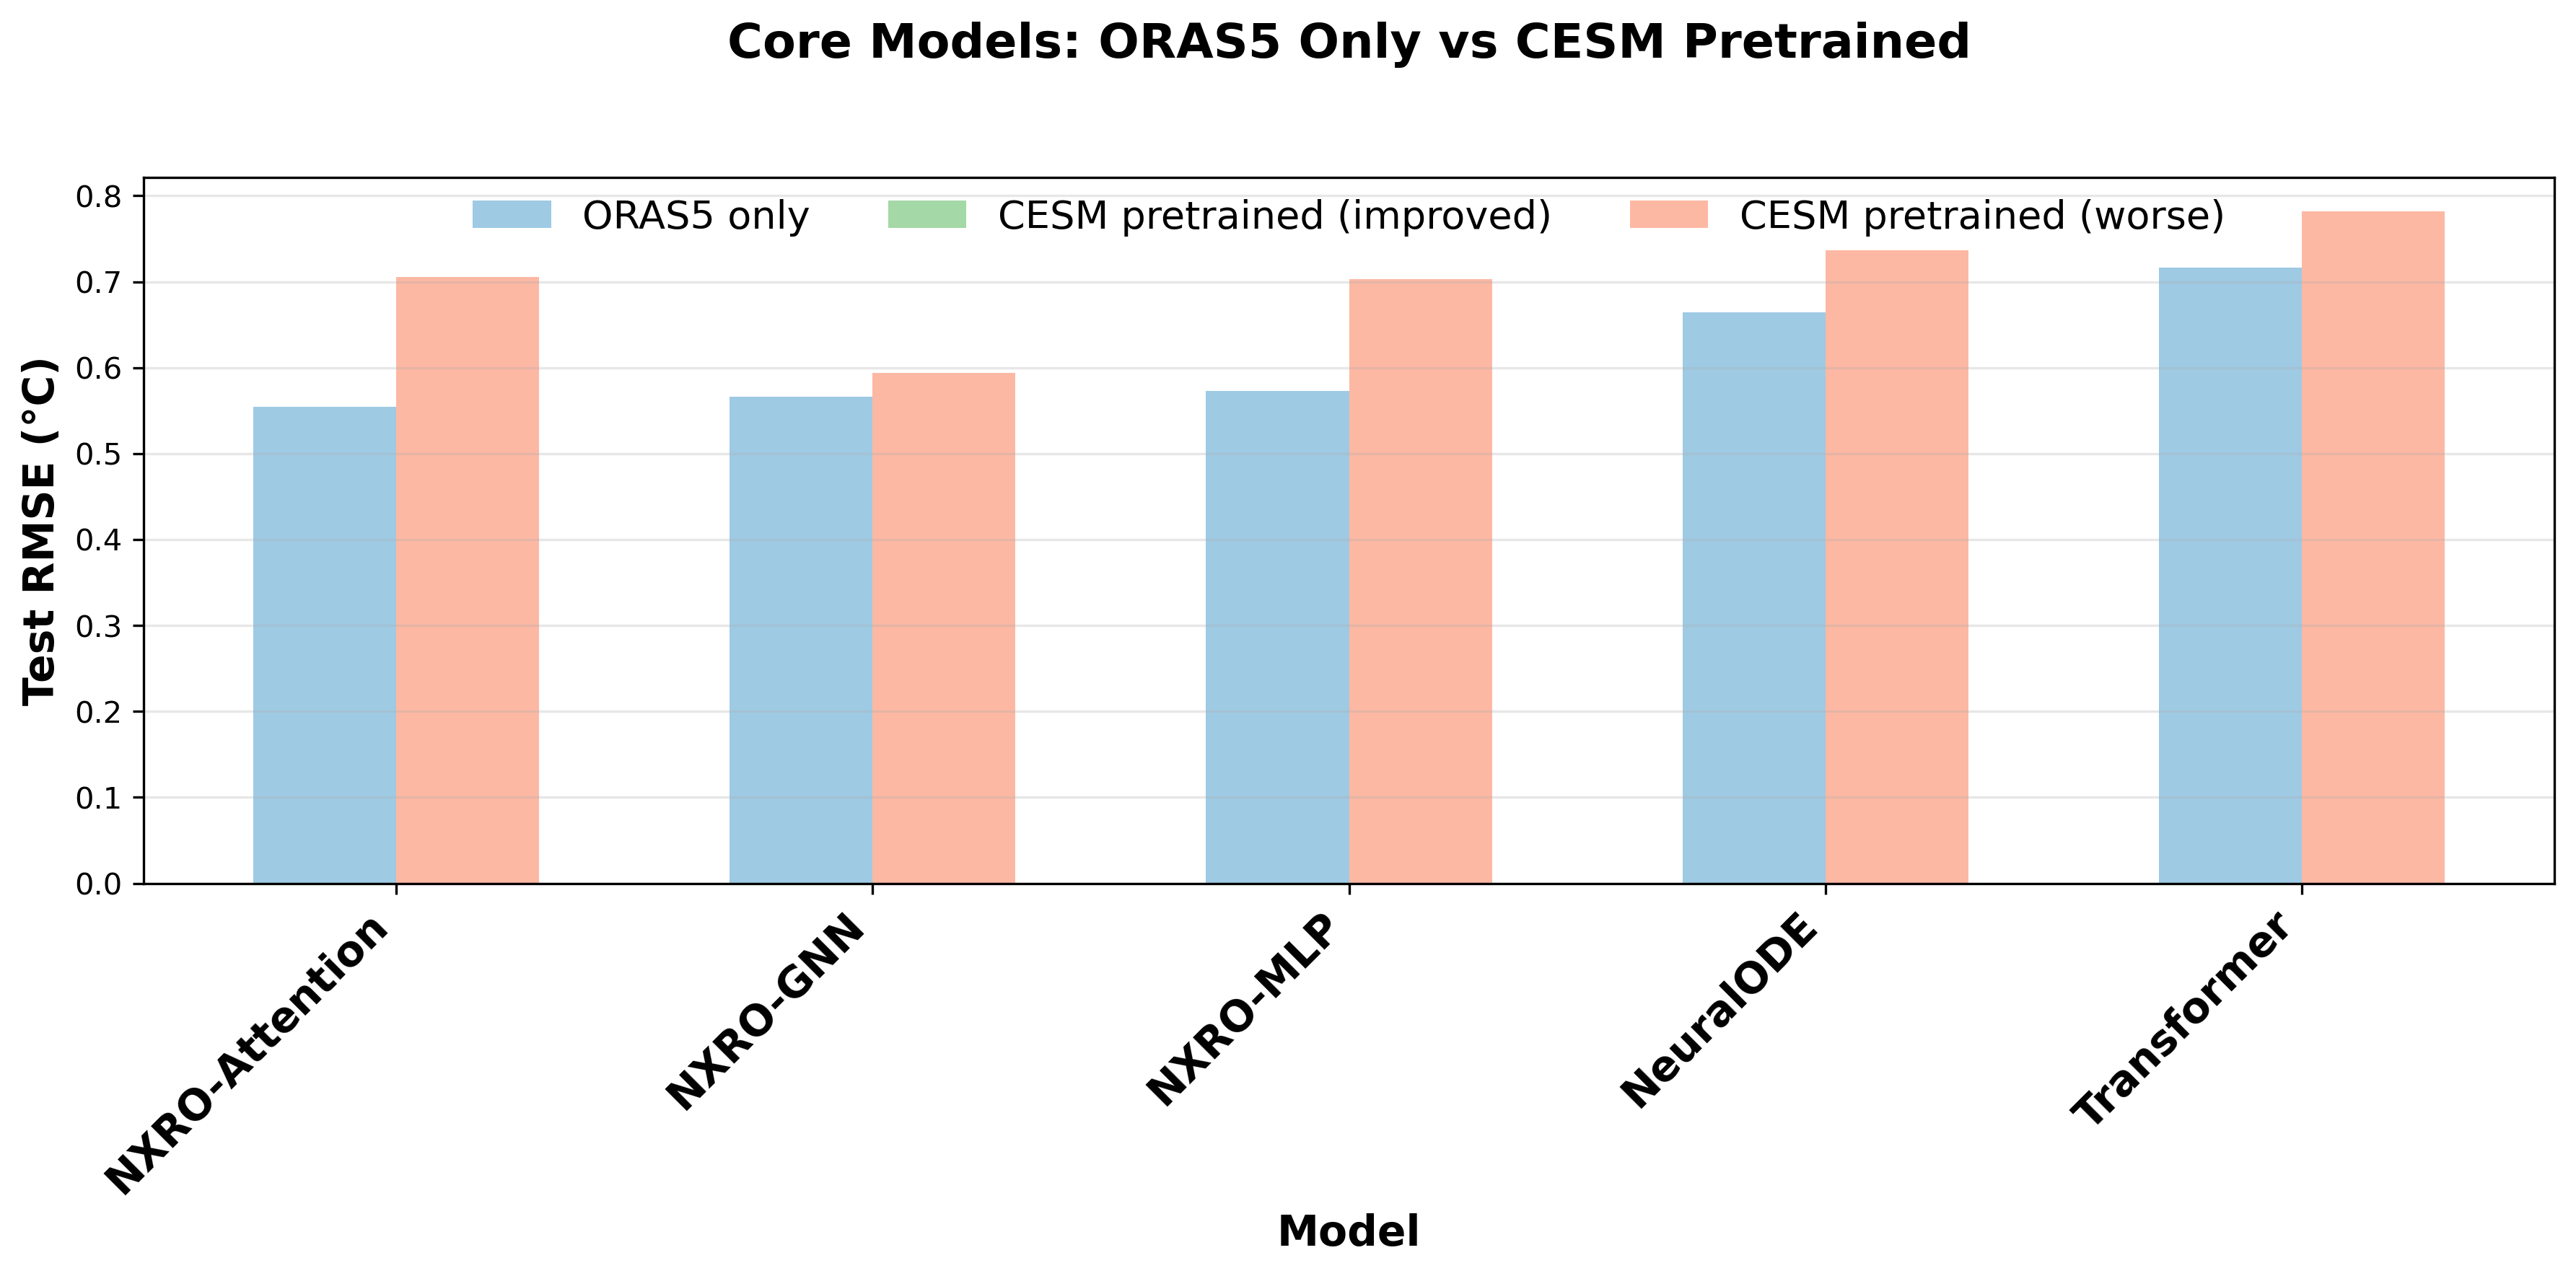
\includegraphics[width=\linewidth]{figures/6d_core_models_single_vs_two_stage.png}
    \caption{Average Test RMSE for ENSO forecast. Comparison of ORAS5 training only vs.\ pretraining on CESM and finetuning on ORAS5. Green bars indicate better performance with CESM; red bars indicate worse.}
    \label{fig:two_stage_a}
\end{figure}




\subsection{Teleconnection Through Graph Structure Learning}

On top of the consistently better performance than the baseline XRO model and the fully nonlinear neural models, our XRO-GNN model defined in equation \ref{eq:nxro_graph} provides the additional benefit of \textit{explainability-by-design}. The mathematical formulation of NXRO-GNN in equation \ref{eq:nxro_graph} includes both the learned linear coupling term $L_\theta(t)$, the nonlinear interaction residual term $\text{GNN}_{\theta}$, and the seasonal gating term $\alpha(t)$. Moreover, the graph structure, encoded by an adjacency matrix, is set to be learnable. By studying these learned components after training, we can hope to uncover the mechanisms discovered by the model that exhibits robust predictive performance. 
    
\begin{figure}[t]
    \centering
    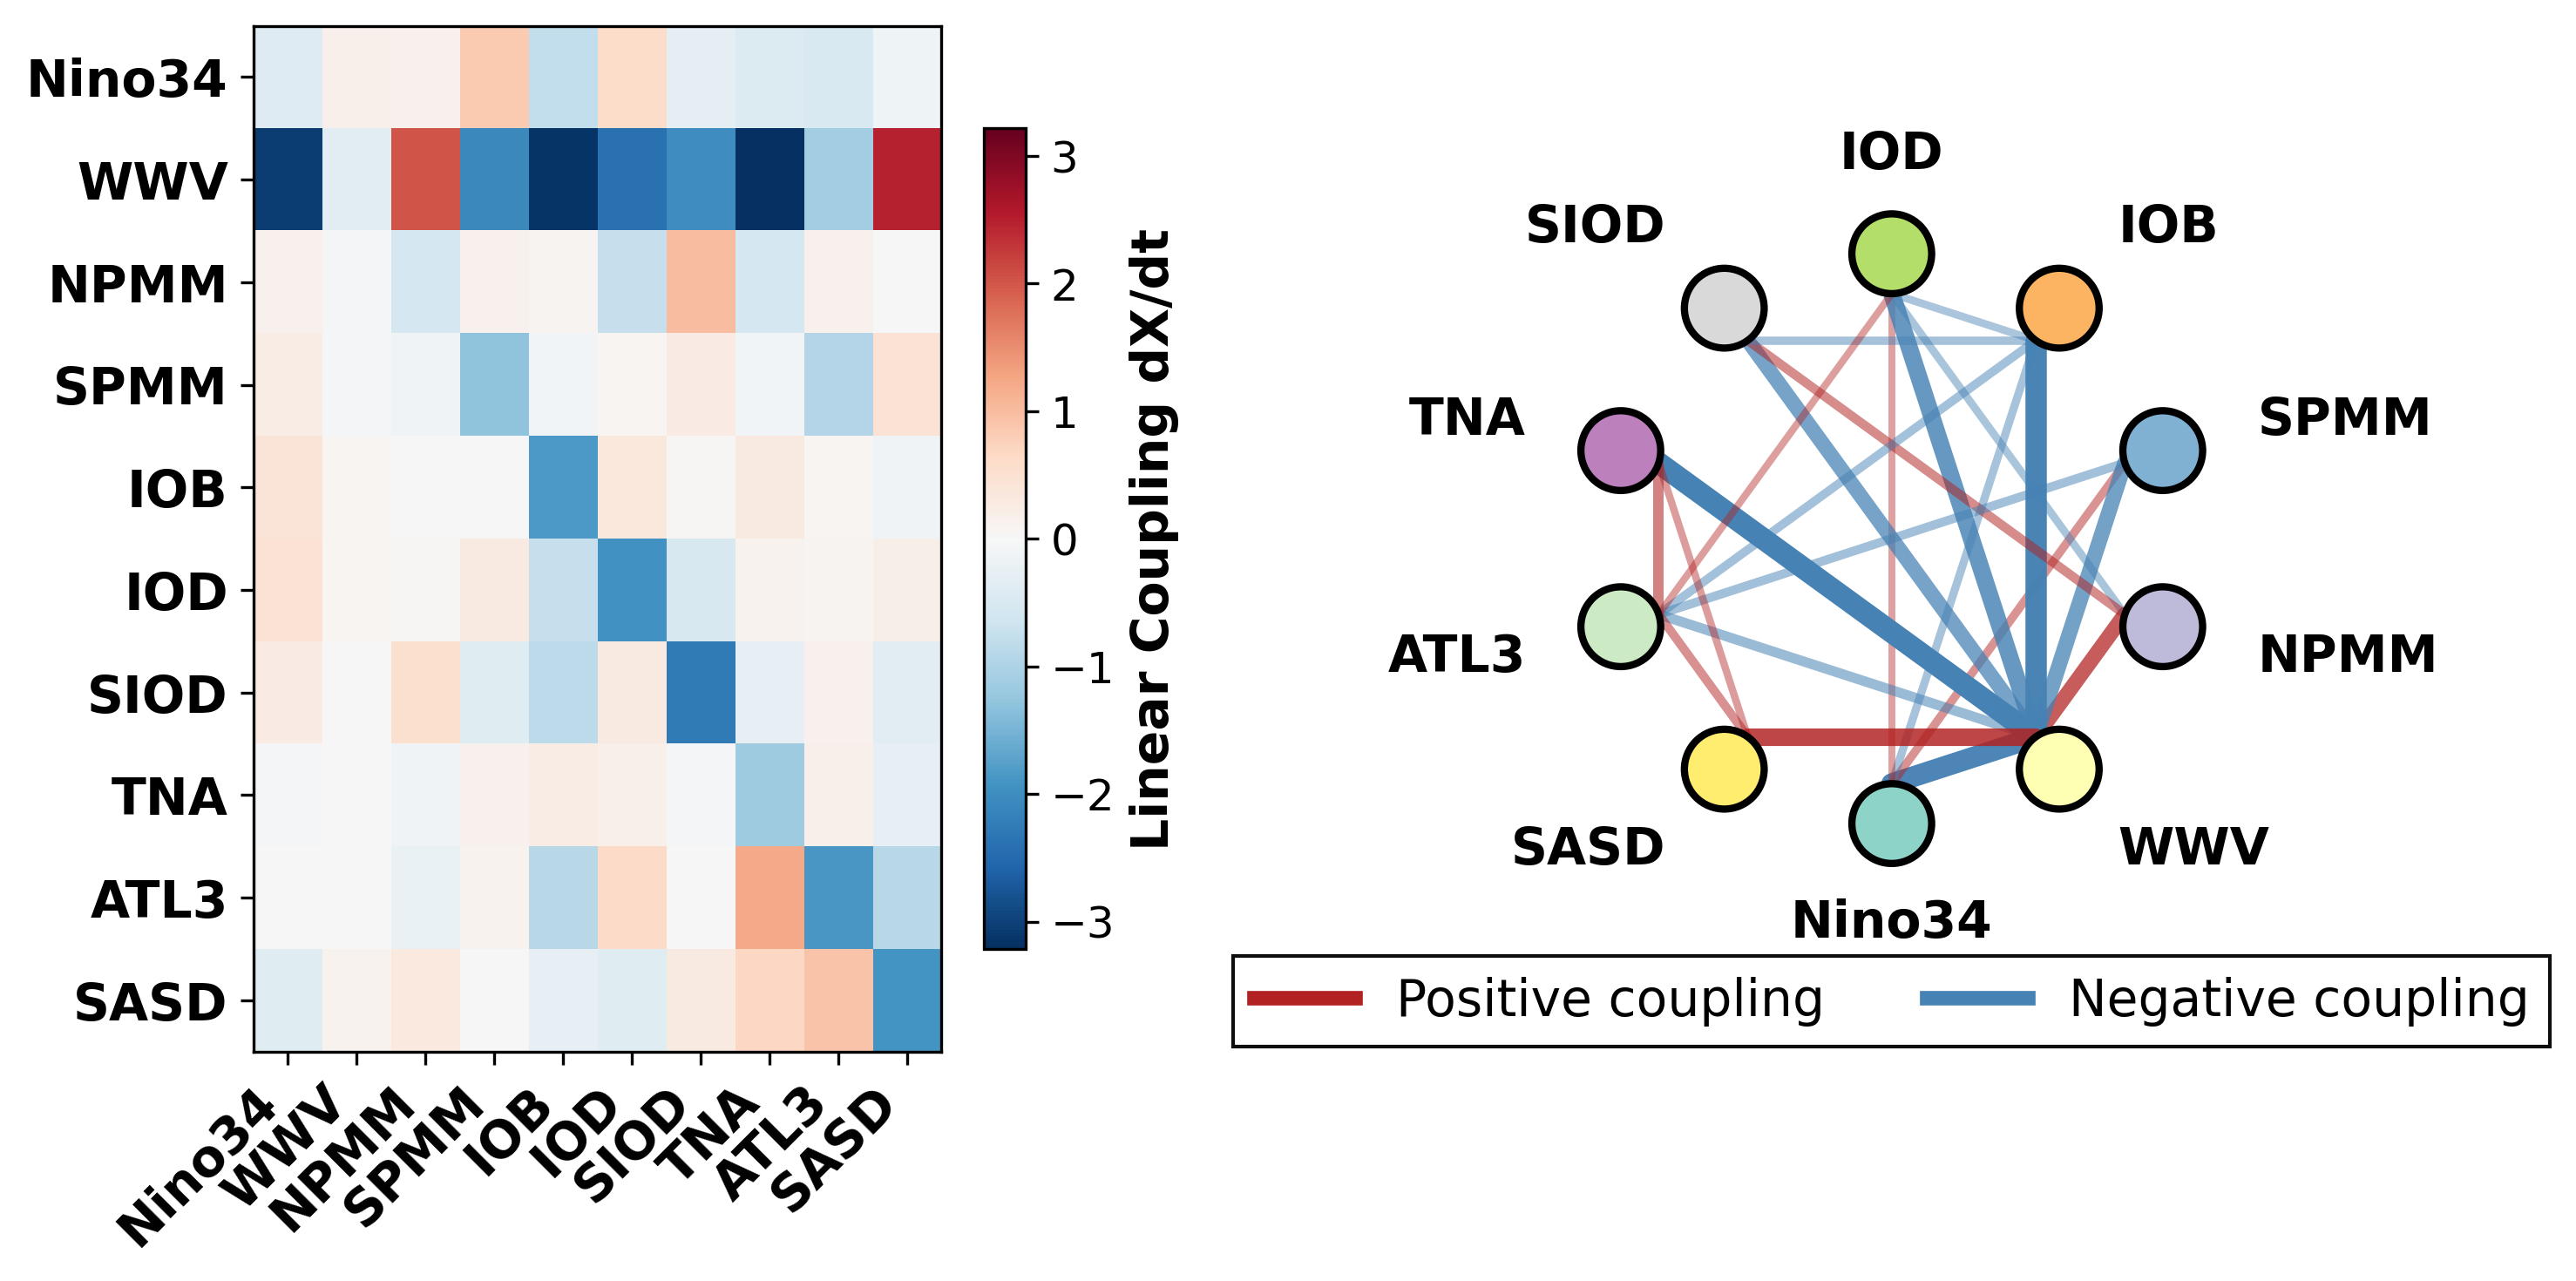
\includegraphics[width=\linewidth]{figures/linear_coupling_L.png}
    \caption{The linear coupling strength between all the climate modes extracted from the learned NXRO-GNN model. Thicker lines and darker color indicates stronger interaction.}
    \label{fig:gnn_linear_coupling}
\end{figure}

\begin{figure}[t]
  \centering
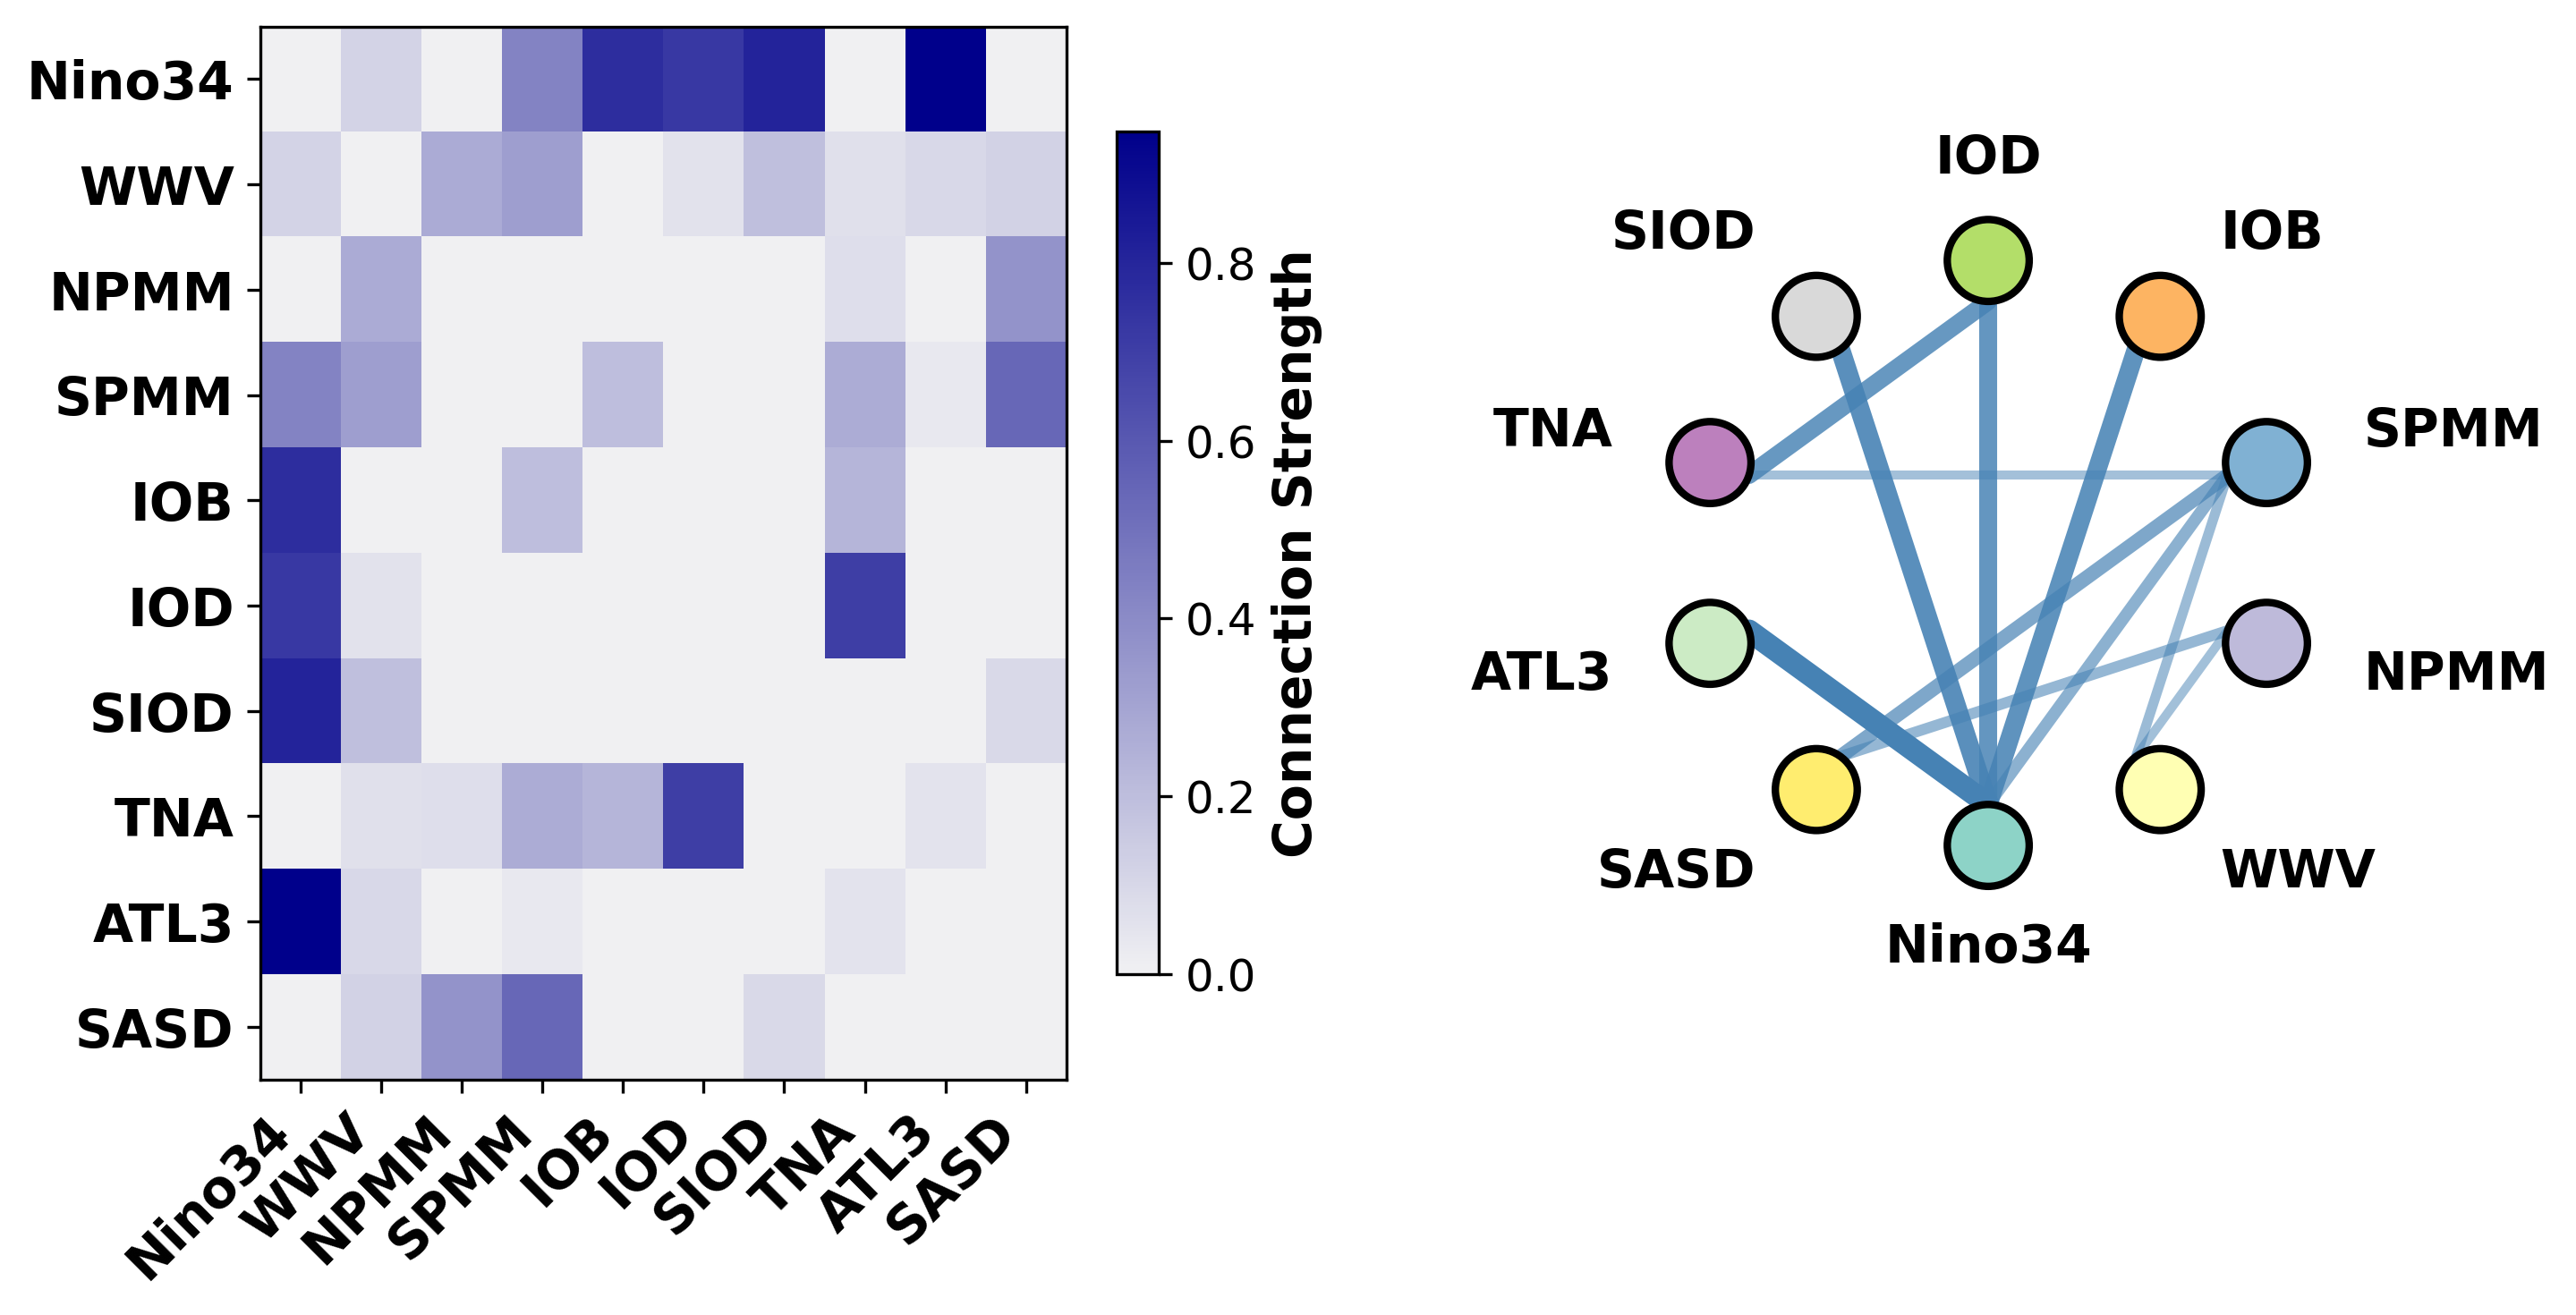
\includegraphics[width=\linewidth]{figures/adjacency_and_network.png}
\caption{The learned graph structure in the residual GNN from a learned NXRO-GNN model. Thicker lines indicate stronger interactions, while color indicates positive and negative interacitons.}
\label{fig:gnn_nonlinear_coupling}
\end{figure}
In Figure \ref{fig:gnn_linear_coupling} and Figure \ref{fig:gnn_nonlinear_coupling} we present the visualization from the learned linear and nonlinear interactions learned by the NXRO-GNN model, which shows that ENSO exhibits weakly linear, but strongly nonlinear interactions with IOD, IOB, SIOD, and ATL3, and in the linear case, much of the influence seems modulated from the coupling with WWV. This result is intriguing, as more recent findings have also hypothesized the strengthened influence  of the Atlantic on ENSO \cite{Zhang2025StrengthenedIO,Wang2024AtlanticWE}, as well as SIOD  \cite{JoHamKug2022SIOD_CPEN}, which in this case seems to be well-captured only with the nonlinear GNN term. In addition, we present the contribution of the nonlinear interactions at each month by plotting the learned seasonal gate values in Figure \ref{fig:seasonal_coupling}, which shows that nonlinear effects are generally stronger in fall and spring. This may partially explain the model's strong performance despite the spring predictability barrier, where linear models tend to perform poorly. 

\begin{figure}
    \centering
    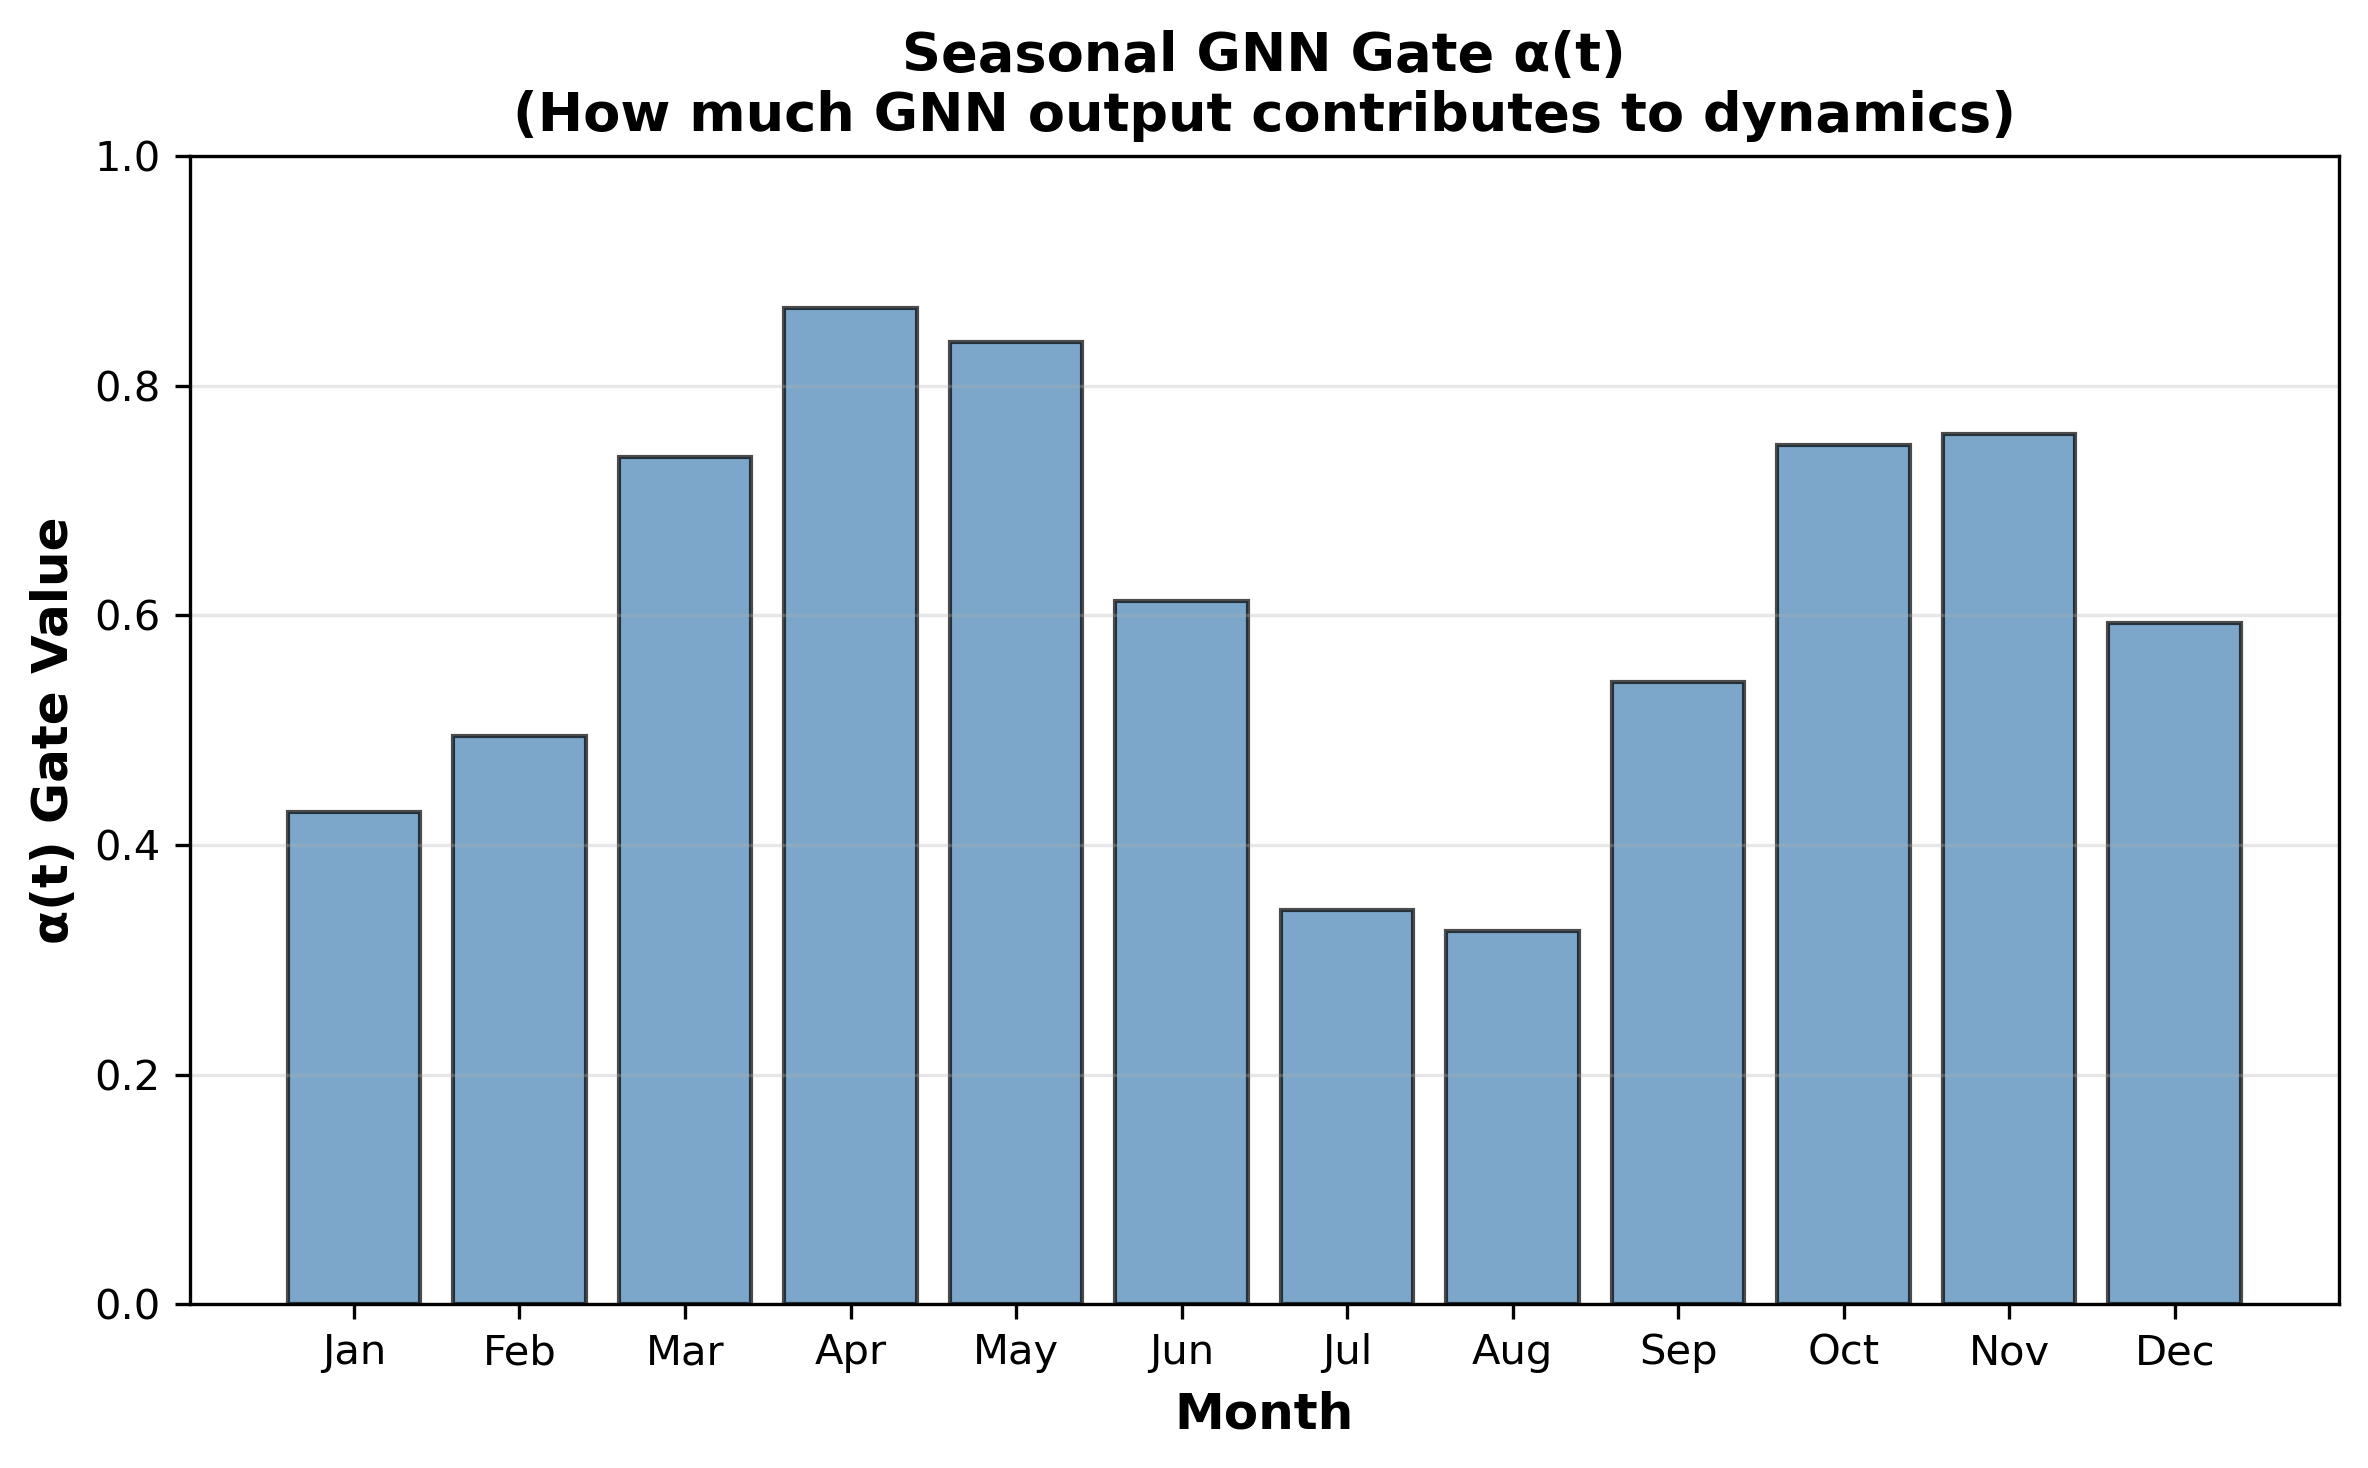
\includegraphics[width=\linewidth]{figures/gcn_seasonal_gate.png}
    \caption{The learned seasonal coupling $\alpha(t)$ for the NXRO-GNN model. Larger values indicate stronger impacts from the nonlinear terms.}
    \label{fig:seasonal_coupling}
\end{figure}







\section{Probabilistic Forecasting with Stochastic Dynamics}
\label{sec:stochastic}

Deterministic forecasts, while useful for point predictions, provide no quantification of uncertainty. Since weather and climate-based forecasts can impact decision-making in applications such as agriculture, water resource management, and disaster preparedness,  probabilistic forecasts that characterize the range of possible outcomes are essential~\cite{gneiting2014probabilistic}. For ENSO specifically, stochastic forcing from atmospheric noise and wind plays a fundamental role in the irregularity of the oscillation~\cite{kleeman2008stochastic}. In this section, we extend the NXRO-Residual framework to generate ensemble forecasts and develop a principled approach to calibrating the stochastic forcing that drives ensemble spread.

\paragraph{Probabilistic Evaluation Metrics: }Evaluating probabilistic forecasts requires metrics that assess both the accuracy of the ensemble mean and the reliability of the uncertainty estimates. We employ the Continuous Ranked Probability Score (CRPS)~\cite{hersbach2000}, a proper scoring rule~\cite{gneiting2007} that generalizes mean absolute error to probabilistic forecasts. The CRPS equals zero for a perfect forecast and increases as the forecast distribution deviates from the observation either in location or spread.  Forecasts that are overconfident (too narrow) are penalized when observations fall in the tails, while forecasts that are underconfident (too wide) are penalized for lacking sharpness. The score is expressed in the same units as the forecast variable (degrees Celsius for temperature), facilitating interpretation. For ensemble forecasts with $M$ members $\{x_1, \ldots, x_M\}$, we employ the fair CRPS estimator that corrects for finite ensemble size:
\begin{equation}
    \text{CRPS} = \frac{1}{M}\sum_{m=1}^{M} |x_m - y| - \frac{1}{2M^2}\sum_{m=1}^{M}\sum_{n=1}^{M} |x_m - x_n|
    \label{eq:crps_fair}
\end{equation}

\paragraph{Stochastic Model Formulation: }A key question in probabilistic forecasting is how to represent the stochastic component that drives ensemble spread. Traditional approaches in numerical weather prediction use stochastically perturbed parameterization tendencies (SPPT)~\cite{buizza1999stochastic}, which multiply physical tendencies by random numbers to represent model uncertainty. For reduced-complexity climate models like XRO~\cite{zhao2024xro}, the standard approach models stochastic forcing as  AR(1) process with seasonally-varying amplitude, fitted post-hoc from model residuals. We adopt this general framework but introduce a likelihood-based optimization procedure that improves upon post-hoc fitting.

In particular, we generate ensemble forecasts by adding stochastic forcing to the deterministic NXRO dynamics. The discrete-time stochastic model takes the form:
\begin{equation}
    \bX_{t+1} = \bX_t + \Delta t \cdot f_\theta(\bX_t, t) + \epsilon_t
    \label{eq:stochastic_model}
\end{equation}
where $f_\theta$ is the deterministic drift (either the full NXRO model or the XRO baseline), $\Delta t = 1/12$ years is the monthly time step, and $\epsilon_t$ is a stochastic perturbation. The perturbation follows a seasonal AR(1) process that captures the temporal correlation and seasonal amplitude modulation observed in forecast residuals:
\begin{equation}
    \epsilon_{j,t} = a_{1,j} \cdot \epsilon_{j,t-1} + \eta_{j,t}, \quad \eta_{j,t} \sim \mathcal{N}(0, (1 - a_{1,j}^2) \cdot \sigma_j(m)^2 \cdot \Delta t^2)
    \label{eq:ar1_noise}
\end{equation}
Here $a_{1,j} \in [0, 1)$ is the AR(1) persistence coefficient for variable $j$, controlling how quickly perturbations decay, and $\sigma_j(m)$ is the noise standard deviation for calendar month $m \in \{1, \ldots, 12\}$, allowing the noise amplitude to vary seasonally. The factor $(1 - a_{1,j}^2)$ ensures that the marginal variance of $\epsilon_{j,t}$ equals $\sigma_j(m)^2 \cdot \Delta t^2$ at stationarity.

% This noise model has $n + 12n$ parameters per model: one persistence coefficient per variable and twelve seasonal standard deviations per variable. The challenge is estimating these parameters in a way that produces well-calibrated ensembles.

\paragraph{Noise Parameter Estimation}

The quality of probabilistic forecasts depends critically on how noise parameters are estimated. Poor calibration---ensembles that are too narrow or too wide---undermines the utility of uncertainty estimates for decision-making~\cite{vannitsem2021statistical}. The XRO model~\cite{zhao2024xro} estimates noise parameters post-hoc by fitting AR(1) models to one-step prediction residuals, an approach that is computationally simple but does not optimize for multi-step forecast calibration. 

\paragraph{Likelihood-Based Optimization:} While post-hoc fitting is computationally convenient, it treats the persistence ($a_1$) and amplitude ($\sigma$) parameters independently, ignoring their joint effect on the stationary distribution. This can lead to suboptimal calibration. Our proposed approach optimizes noise parameters via maximum likelihood while holding the dynamics model fixed. This two-stage procedure separates the learning of deterministic dynamics from stochastic parameters, similar in spirit to approaches in neural stochastic differential equations~\cite{li2020scalable,kidger2021neural}. Given residuals $\{r_t\}_{t=1}^{T}$ computed from the frozen model, the conditional log-likelihood under the AR(1) model is:
\begin{equation}
    \ell(a_1, \sigma) = \sum_{t=2}^{T} \log p(r_t | r_{t-1}; a_1, \sigma_{m_t})
\end{equation}
where $m_t$ denotes the calendar month at time $t$ and $p(r_t | r_{t-1}; a_1, \sigma)$ is the Gaussian density implied by Equation~\ref{eq:ar1_noise}. We maximize this likelihood using gradient ascent, initializing from the post-hoc estimates. Unlike post-hoc fitting, it accounts for the interaction between persistence and amplitude. We refer to this as \textit{Stage 2} fitting because it occurs after the dynamics model has been trained (Stage 1 being the deterministic fitting described in Section~\ref{sec:neural_ode}).

\subsection{Results}

\begin{figure*}[t]
  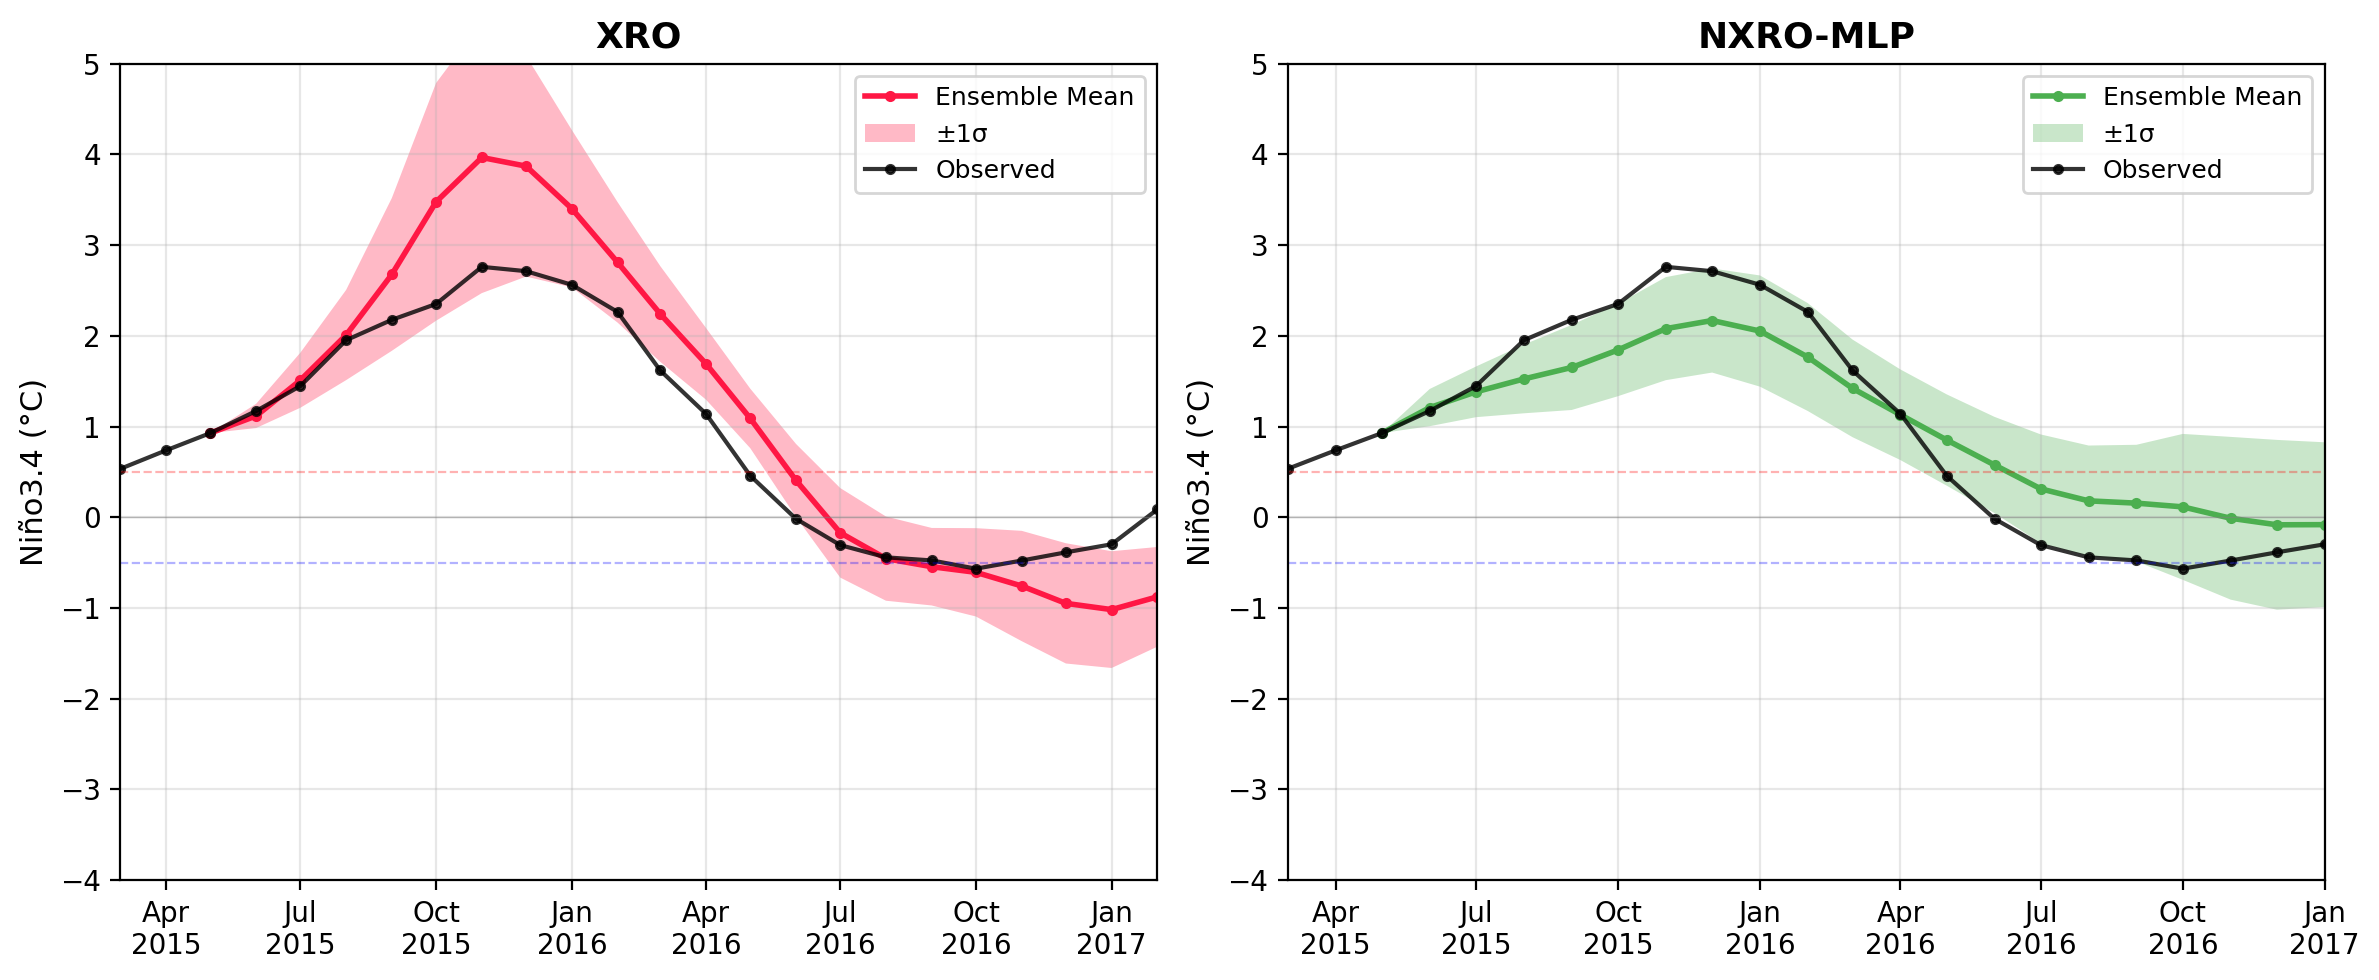
\includegraphics[width=\linewidth]{figures/elnino_2015_spring_xro_vs_mlp.png}
  \caption{Ensemble forecast comparison for the 2015 El Nino Spring development. Shaded regions show 10--90\% quantile ranges; solid lines show ensemble median; dots show observations. The NXRO-MLP model exhibits wider, better-calibrated spread.}
  \label{fig:forecast_samples_outsample}
\end{figure*}


Table ~\ref{tab:stochastic_outsample} presents the stochastic forecast performance for the out-of-sample evaluation. The results reveal striking differences between the noise estimation approaches. All NXRO variants with Stage 2 noise optimization outperform the XRO baseline, with up-to 13.0\% improvement in CRPS, achieved by the NXRO-GNN model, which is a meaningful advance for operational forecasting. In addition to CRPS, we also report Spread over RMSE, calculated as the ratio between standard deviation of ensemble forecasts and RMSE of the ensemble mean, averaged over all the lead times. The XRO baseline achieves a spread-to-RMSE ratio of only 0.527, indicating that its ensembles are overconfident. Stage 2 optimization increases this ratio to 0.625-0.654 across NXRO variants, moving closer to the ideal of 1.0. Better calibration means that users can more reliably interpret the ensemble spread as representing forecast uncertainty. %\YS{define spread to rmse. use the same term in Table 2. }

\begin{table}[h]
\setlength{\tabcolsep}{1pt}
\centering
\caption{Stochastic ensemble forecast performance for NXRO and XRO. Higher CRPS metrics means better calibration. }
\label{tab:stochastic_outsample}
\resizebox{\columnwidth}{!}{
\begin{tabular}{lcccc}
\toprule
\textbf{Model} & \textbf{CRPS} 
& \textbf{\shortstack{Ensemble\\RMSE}} 
& \textbf{\shortstack{Spread \\ over RMSE}} 
& \textbf{\shortstack{vs. \\ XRO}} \\
\midrule
NXRO-GNN & \textbf{0.488} & \textbf{0.899°C} & \textbf{0.654} & \textbf{$-$13.0\%} \\
NXRO-Attentive & 0.513 & 0.901°C & 0.634 & $-$8.6\% \\
NXRO-MLP & 0.548 & 0.963°C & 0.625 & $-$2.4\% \\
XRO & 0.561 & 0.970°C & 0.527 & --- \\
\bottomrule
\end{tabular}
}
\end{table}
\vspace{-9pt}
\subsection{Forecast Visualization}

Figure~\ref{fig:forecast_samples_outsample} illustrates an example of stochastic forecast with XRO and NXRO-MLP through ensemble plumes. The XRO ensemble (left panel) exhibits wide spreads that result in excessive uncertainty estimate, while missing observations. The NXRO-MLP ensemble (right panel) shows appropriately tighter spread that better represents forecast uncertainty while maintaining a more accurate ensemble mean, fitting the observations shape better and exhibiting better calibration. Additional stochastic forecast results can be found in Appendix B.



% TODO: add related works ection.
% \section{Related Works}

The study of using optimal transport \cite{Villani2008OptimalTO} to improve flow matching was proposed firstly in \cite{tong2024improvinggeneralizingflowbasedgenerative, pooladian2023multisampleflowmatchingstraightening}, which adds optimal transport induced coupling for the minibatch before the interpolation and model training step. Several follow-up works \cite{kornilov2024optimalflowmatchinglearning, yue2025oatfmoptimalaccelerationtransport} have aimed to further expand the framework. All have assumed that the sample space is $\mathbb{R}^d$. In order to better capture the resolution-invariance of grid data and continuity of path data, Functional Flow Matching \cite{kerrigan2023functionalflowmatching} first proposed a framework to do flow matching in Hilbert space, relying on Gaussian measure theory. However, the same optimal transport acceleration has not been made in this space.

The line of research that embeds probability measures in RKHS has been proposed by the pioneering work of \cite{Sriperumbudur2010Hilbert, gretton2008kernelmethodtwosampleproblem}, where the kernel-induced metrics, called Intergral Probability Metrics (IPM), has been studied extensively \cite{Dudley_2002, Sriperumbudur2010Hilbert} and used for two-sample  hypothesis testing \cite{gretton2008kernelmethodtwosampleproblem}, most recently in path space \cite{chevyrev2022signaturemoments}. IPW in the form of Maximum Mean Discrepancy (MMD) has been linked with both probability divergence and Wasserstein distance \cite{feydy19a-pmlr} and has seen clear entropic optimal transport formulation in \cite{Li_2021_CVPR} in the form of Hilbert Sinkhorn Divergence and a gradient flow formulation in \cite{galashov2024deepmmdgradientflow, arbel2019maximummeandiscrepancygradient}. Nevertheless, the extension of these frameworks to function space is an active area of research in mathematics, and our work presents the first to explore it in the context of flow matching. 

\section{Conclusion}
\label{sec:conclusion}

We presented the Neural Residual ODE framework for ENSO forecasting, systematically investigating how to combine physics-based structure with machine learning flexibility for climate prediction under severe data limitations. Our model, NXRO, and its 43 model variants, are evaluated on rigorous out-of-sample forecasting and yield insights relevant to both the climate science and machine learning communities. The central result of this work is that simple hybrid architectures outperform both the full physics-based XRO model and pure nonlinear deep learning approaches when the observational dataset is scarce, and adding synthetic climate simulation data can introduce systematic biases that hamper the model performance. This result carries implications for practitioners: modern deep learning architectures do not automatically transfer to small-data scientific domains, and the choice of synthetic datasets matter. The hybrid approach, which encodes well-understood physics as architectural structure while learning corrections from data, emerges as the optimal strategy for the small-data regime characteristic of climate science and many other scientific domains. In practice, it points to a strategy to construct a physically meaningful and accurate model without relying on massive scale simulations. % We hope to extend this framework to application to other scientific domains, such as fluid and molecular dynamics, and other climate indices. 


\section{Limitations and Ethical Considerations}

Our results speak to ongoing debates about the role of physics in AI4science and demonstrates that for the task of ENSO forecasting, a physics-inspired simple neural model can outperform fully nonlinear neural models, even with additional simulation data. Nevertheless, our study is limited to ENSO forecast, and we hope to extend it to other scientific domains, such as fluid and molecular dynamics, and other climate indices. In addition, since the choice of synthetic datasets matter, we hope to more thoroughly examine other climate simulation datasets as well. For the ethical implications, we are not aware of any issues related to data privacy, consent, bias, and potential misuses. Our dataset will be open sourced, consisting of observation data and climate model simulations, none of which has ethical implications. 

% \section*{Impact Statement}

% Authors are \textbf{required} to include a statement of the potential broader
% impact of their work, including its ethical aspects and future societal
% consequences. This statement should be in an unnumbered section at the end of
% the paper (co-located with Acknowledgements -- the two may appear in either
% order, but both must be before References), and does not count toward the paper
% page limit. In many cases, where the ethical impacts and expected societal
% implications are those that are well established when advancing the field of
% Machine Learning, substantial discussion is not required, and a simple
% statement such as the following will suffice:

% ``This paper presents work whose goal is to advance the field of Machine
% Learning. There are many potential societal consequences of our work, none
% which we feel must be specifically highlighted here.''

% The above statement can be used verbatim in such cases, but we encourage
% authors to think about whether there is content which does warrant further
% discussion, as this statement will be apparent if the paper is later flagged
% for ethics review.

\clearpage
\bibliographystyle{ACM-Reference-Format}
\bibliography{references}


% \section{Acknowledgments}
% Identification of funding sources and other support, and thanks to
% individuals and groups that assisted in the research and the
% preparation of the work should be included in an acknowledgment
% section, which is placed just before the reference section in your
% document.

% This section has a special environment:
% \begin{verbatim}
%   \begin{acks}
%   ...
%   \end{acks}
% \end{verbatim}
% so that the information contained therein can be more easily collected
% during the article metadata extraction phase, and to ensure
% consistency in the spelling of the section heading.

% Authors should not prepare this section as a numbered or unnumbered {\verb|\section|}; please use the ``{\verb|acks|}'' environment.


\newpage
\appendix
\onecolumn

\section{Additional Experimental Results}


In this section, we provide comprehensive experimental results through our extensive neural architectural search. 



\subsection{All Neural Models} \label{app:a1}

All NXRO models share a common structure: they learn a vector field $f_\theta(X, t)$ that defines an ordinary differential align* (ODE) for the state evolution:
\begin{align*}
    \frac{dX}{dt} = f_\theta(X, t)
\end{align*}
where $X \in \mathbb{R}^d$ is the state vector containing climate indices (e.g., Ni\~no3.4, WWV, NPMM, etc.), $t$ is time in years, and $\theta$ represents learnable parameters. All models use a Fourier time embedding to capture seasonality:
\begin{align*}
    \phi(t) = \left[1, \cos(\omega t), \sin(\omega t), \ldots, \cos(K\omega t), \sin(K\omega t)\right]^\top \in \mathbb{R}^{1+2K}
\end{align*}
with $\omega = 2\pi$ (annual cycle) and $K=2$ (default) giving 5 basis functions.

\textbf{Default Hyperparameters:} Epochs: 2000, batch size: 128, learning rate: $10^{-3}$, weight decay: $10^{-4}$, $K=2$.

%==============================================================================
\paragraph{NXRO-Linear.}
A purely linear model with seasonally-varying linear operator.
\begin{align*}
    \frac{dX}{dt} = L_\theta(t) \cdot X, \quad L_\theta(t) = \sum_{k=0}^{2K} W_k \cdot \phi_k(t)
\end{align*}
where $W_k \in \mathbb{R}^{d \times d}$ are learnable weight matrices. \textbf{Params:} $5d^2$.

\begin{tabular}{@{}ll@{}}
\textbf{Variant} & \textbf{Description} \\
\hline
NXRO-Linear & Random Xavier initialization \\
NXRO-Linear-WS & Warm-start from XRO linear operator \\
\end{tabular}

%==============================================================================
\paragraph{NXRO-RO.}
Seasonal linear operator plus Recharge Oscillator (RO) nonlinear terms on $(T, H)$.
\begin{align*}
    \frac{dX}{dt} = L_\theta(t) \cdot X + \begin{bmatrix} \text{RO}_T(T,H,t) \\ \text{RO}_H(T,H,t) \\ 0 \\ \vdots \end{bmatrix}, \quad
    \text{RO}_T = \sum_{k} c^T_k(t) \cdot \psi_k(T,H)
\end{align*}
with $\psi = [T^2, TH, T^3, T^2H, TH^2]^\top$ and seasonally-varying coefficients.

%==============================================================================
\paragraph{NXRO-RO+Diag.}
Extends NXRO-RO with diagonal quadratic and cubic terms for all variables.
\begin{align*}
    \frac{dX}{dt} = L_\theta(t) \cdot X + \text{RO}(T,H,t) + b(t) \odot X^2 + c(t) \odot X^3
\end{align*}

\begin{tabular}{@{}ll@{}}
\textbf{Variant} & \textbf{Description} \\
\hline
NXRO-RO+Diag & Random initialization \\
NXRO-RO+Diag-WS & Warm-start all, train all \\
NXRO-RO+Diag-FixL & Freeze linear, train RO+Diag \\
NXRO-RO+Diag-FixRO & Freeze RO, train linear+Diag \\
NXRO-RO+Diag-FixDiag & Freeze diagonal, train linear+RO \\
NXRO-RO+Diag-FixNL & Freeze RO+Diag, train linear only \\
\end{tabular}

%==============================================================================
\paragraph{NXRO-MLP.}
Seasonal linear operator plus a residual 2-layer MLP.
\begin{align*}
    \frac{dX}{dt} = L_\theta(t) \cdot X + R_\theta([X, \phi(t)]), \quad
    R_\theta(z) = W_3 \tanh(W_2 \tanh(W_1 z))
\end{align*}
\textbf{Hyperparams:} Hidden: 64, 2 layers, $\tanh$ activation.

\begin{tabular}{@{}ll@{}}
\textbf{Variant} & \textbf{Description} \\
\hline
NXRO-MLP & Random initialization \\
NXRO-MLP-WS-FixL & Warm-start \& freeze linear, train MLP only \\
\end{tabular}

%==============================================================================
\paragraph{NXRO-DeepMLP.}
General neural ODE with configurable-depth drift MLP and optional structural constraints.
\begin{align*}
    \frac{dX}{dt} = L_\theta(t) \cdot X + G_\theta([X, \phi(t)]) + M \cdot X
\end{align*}
where $G_\theta$ is a deeper MLP and $M$ is an optional masked linear mixing term.

%==============================================================================
\paragraph{NXRO-PhysReg.}
Neural ODE with physics-informed regularization via Jacobian penalty.
\begin{align*}
    \mathcal{L} = \mathcal{L}_{\text{MSE}} + \lambda_{\text{jac}} \|\nabla_X f_\theta(X,t)\|_F^2
\end{align*}
\textbf{Hyperparams:} Same as NXRO-DeepMLP, $\lambda_{\text{jac}} = 10^{-4}$.

%==============================================================================
\paragraph{NXRO-HybridMLP.}
Combines the interpretable RO+Diag structure with a scaled residual MLP.
\begin{align*}
    \frac{dX}{dt} = f_{\text{RO+Diag}}(X,t) + \alpha \cdot R_\theta([X, \phi(t)])
\end{align*}
\textbf{Hyperparams:} Hidden: 64, $\alpha_{\text{init}} = 0.1$, $\alpha_{\max} = 0.5$.

\begin{tabular}{@{}ll@{}}
\textbf{Variant} & \textbf{Description} \\
\hline
NXRO-HybridMLP & Random initialization \\
NXRO-HybridMLP-WS & Warm-start physics, train all \\
NXRO-HybridMLP-FixPhysics & Freeze RO+Diag, train MLP only \\
NXRO-HybridMLP-FixRO & Freeze RO terms only \\
NXRO-HybridMLP-FixNL & Freeze all nonlinear physics \\
\end{tabular}

%==============================================================================
\paragraph{NXRO-Bilinear.}
Seasonal linear plus low-rank bilinear channels with seasonal gating.
\begin{align*}
    \frac{dX}{dt} = L_\theta(t) \cdot X + \sum_{c=1}^{C} \alpha_c(t) \cdot s_c(X) \cdot W^{(c)}_{\text{proj}}
\end{align*}
where $s_c(X) = \sum_r (P_c^\top X)_r (Q_c^\top X)_r$ are bilinear scalars. \textbf{Hyperparams:} Channels: 2, rank: 2.

%==============================================================================
\paragraph{NXRO-Attention.}
Seasonal linear plus lightweight self-attention across variables.
\begin{align*}
    \frac{dX}{dt} = L_\theta(t) \cdot X + \alpha(t) \cdot \text{Proj}\left(\text{softmax}\left(\frac{M \odot QK^\top}{\sqrt{d_k}}\right) V\right)
\end{align*}
\textbf{Hyperparams:} $d=32$, single head. \textbf{Mask:} \texttt{th\_only} (attend from $T,H$) or \texttt{full}.

\begin{tabular}{@{}ll@{}}
\textbf{Variant} & \textbf{Description} \\
\hline
NXRO-Attention & Random initialization \\
NXRO-Attention-WS & Warm-start linear, train all \\
NXRO-Attention-FixL & Freeze linear, train attention only \\
\end{tabular}

%==============================================================================
\paragraph{NXRO-Graph.}
Seasonal linear plus sparse graph-based drift.
\begin{align*}
    \frac{dX}{dt} = L_\theta(t) \cdot X + \alpha(t) \cdot \tanh\left(\hat{A} X \cdot W_g\right)
\end{align*}
where $\hat{A}$ is a row-normalized adjacency matrix. \textbf{Hyperparams:} Top-$k$: 2.

\begin{tabular}{@{}ll@{}}
\textbf{Variant} & \textbf{Description} \\
\hline
NXRO-Graph-Fixed & Fixed adjacency from XRO or correlation \\
NXRO-Graph-Learned & Learnable adjacency with L1 reg ($\lambda_1 = 0.01$) \\
\end{tabular}

%==============================================================================
\paragraph{NXRO-GCN.}
PyTorch Geometric-based Graph ODE using Graph Convolutional Networks. This is the NXRO-GNN model in the main paper.

\begin{align*}
    \frac{dX}{dt} = L_\theta(t) \cdot X + \alpha(t) \cdot \text{GCN}_\theta(X, \mathcal{E})
\end{align*}
Two GCNConv layers with $\tanh$ activation. \textbf{Hyperparams:} Hidden: 16, top-$k$: 3, dropout: 0.1.

%==============================================================================
\paragraph{NXRO-GAT.}
PyTorch Geometric-based Graph ODE using Graph Attention Networks.
\begin{align*}
    \frac{dX}{dt} = L_\theta(t) \cdot X + \alpha(t) \cdot \text{GAT}_\theta(X, \mathcal{E})
\end{align*}
Same as NXRO-GCN but uses GATConv with attention-weighted message passing:
\begin{align*}
    h_i = \sigma\left(\sum_{j \in \mathcal{N}(i)} \alpha_{ij} W h_j\right), \quad \alpha_{ij} \propto \exp(\text{LeakyReLU}(a^\top [Wh_i \| Wh_j]))
\end{align*}
\textbf{Hyperparams:} Hidden: 16, top-$k$: 3, dropout: 0.1.

%==============================================================================
\paragraph{NXRO-Transformer.}
Pure Transformer architecture treating each variable as a token.
\begin{align*}
    \frac{dX}{dt} = \text{OutputProj}\left(\text{TransformerEncoder}\left(\text{InputProj}([X_i, \phi(t)]) + p_i\right)_{i=1}^d\right)
\end{align*}
where $p_i$ is a learnable positional embedding for variable $i$.
\textbf{Hyperparams:} $d_{\text{model}}$: 64, heads: 4, layers: 2, FFN dim: 256, dropout: 0.1, GELU.

The comprehensive results of all model ranking, trained only on the ORAS5 dataset, can be found in Figure \ref{fig:all_models_rmse_ranking}.

\begin{figure}
    \centering
    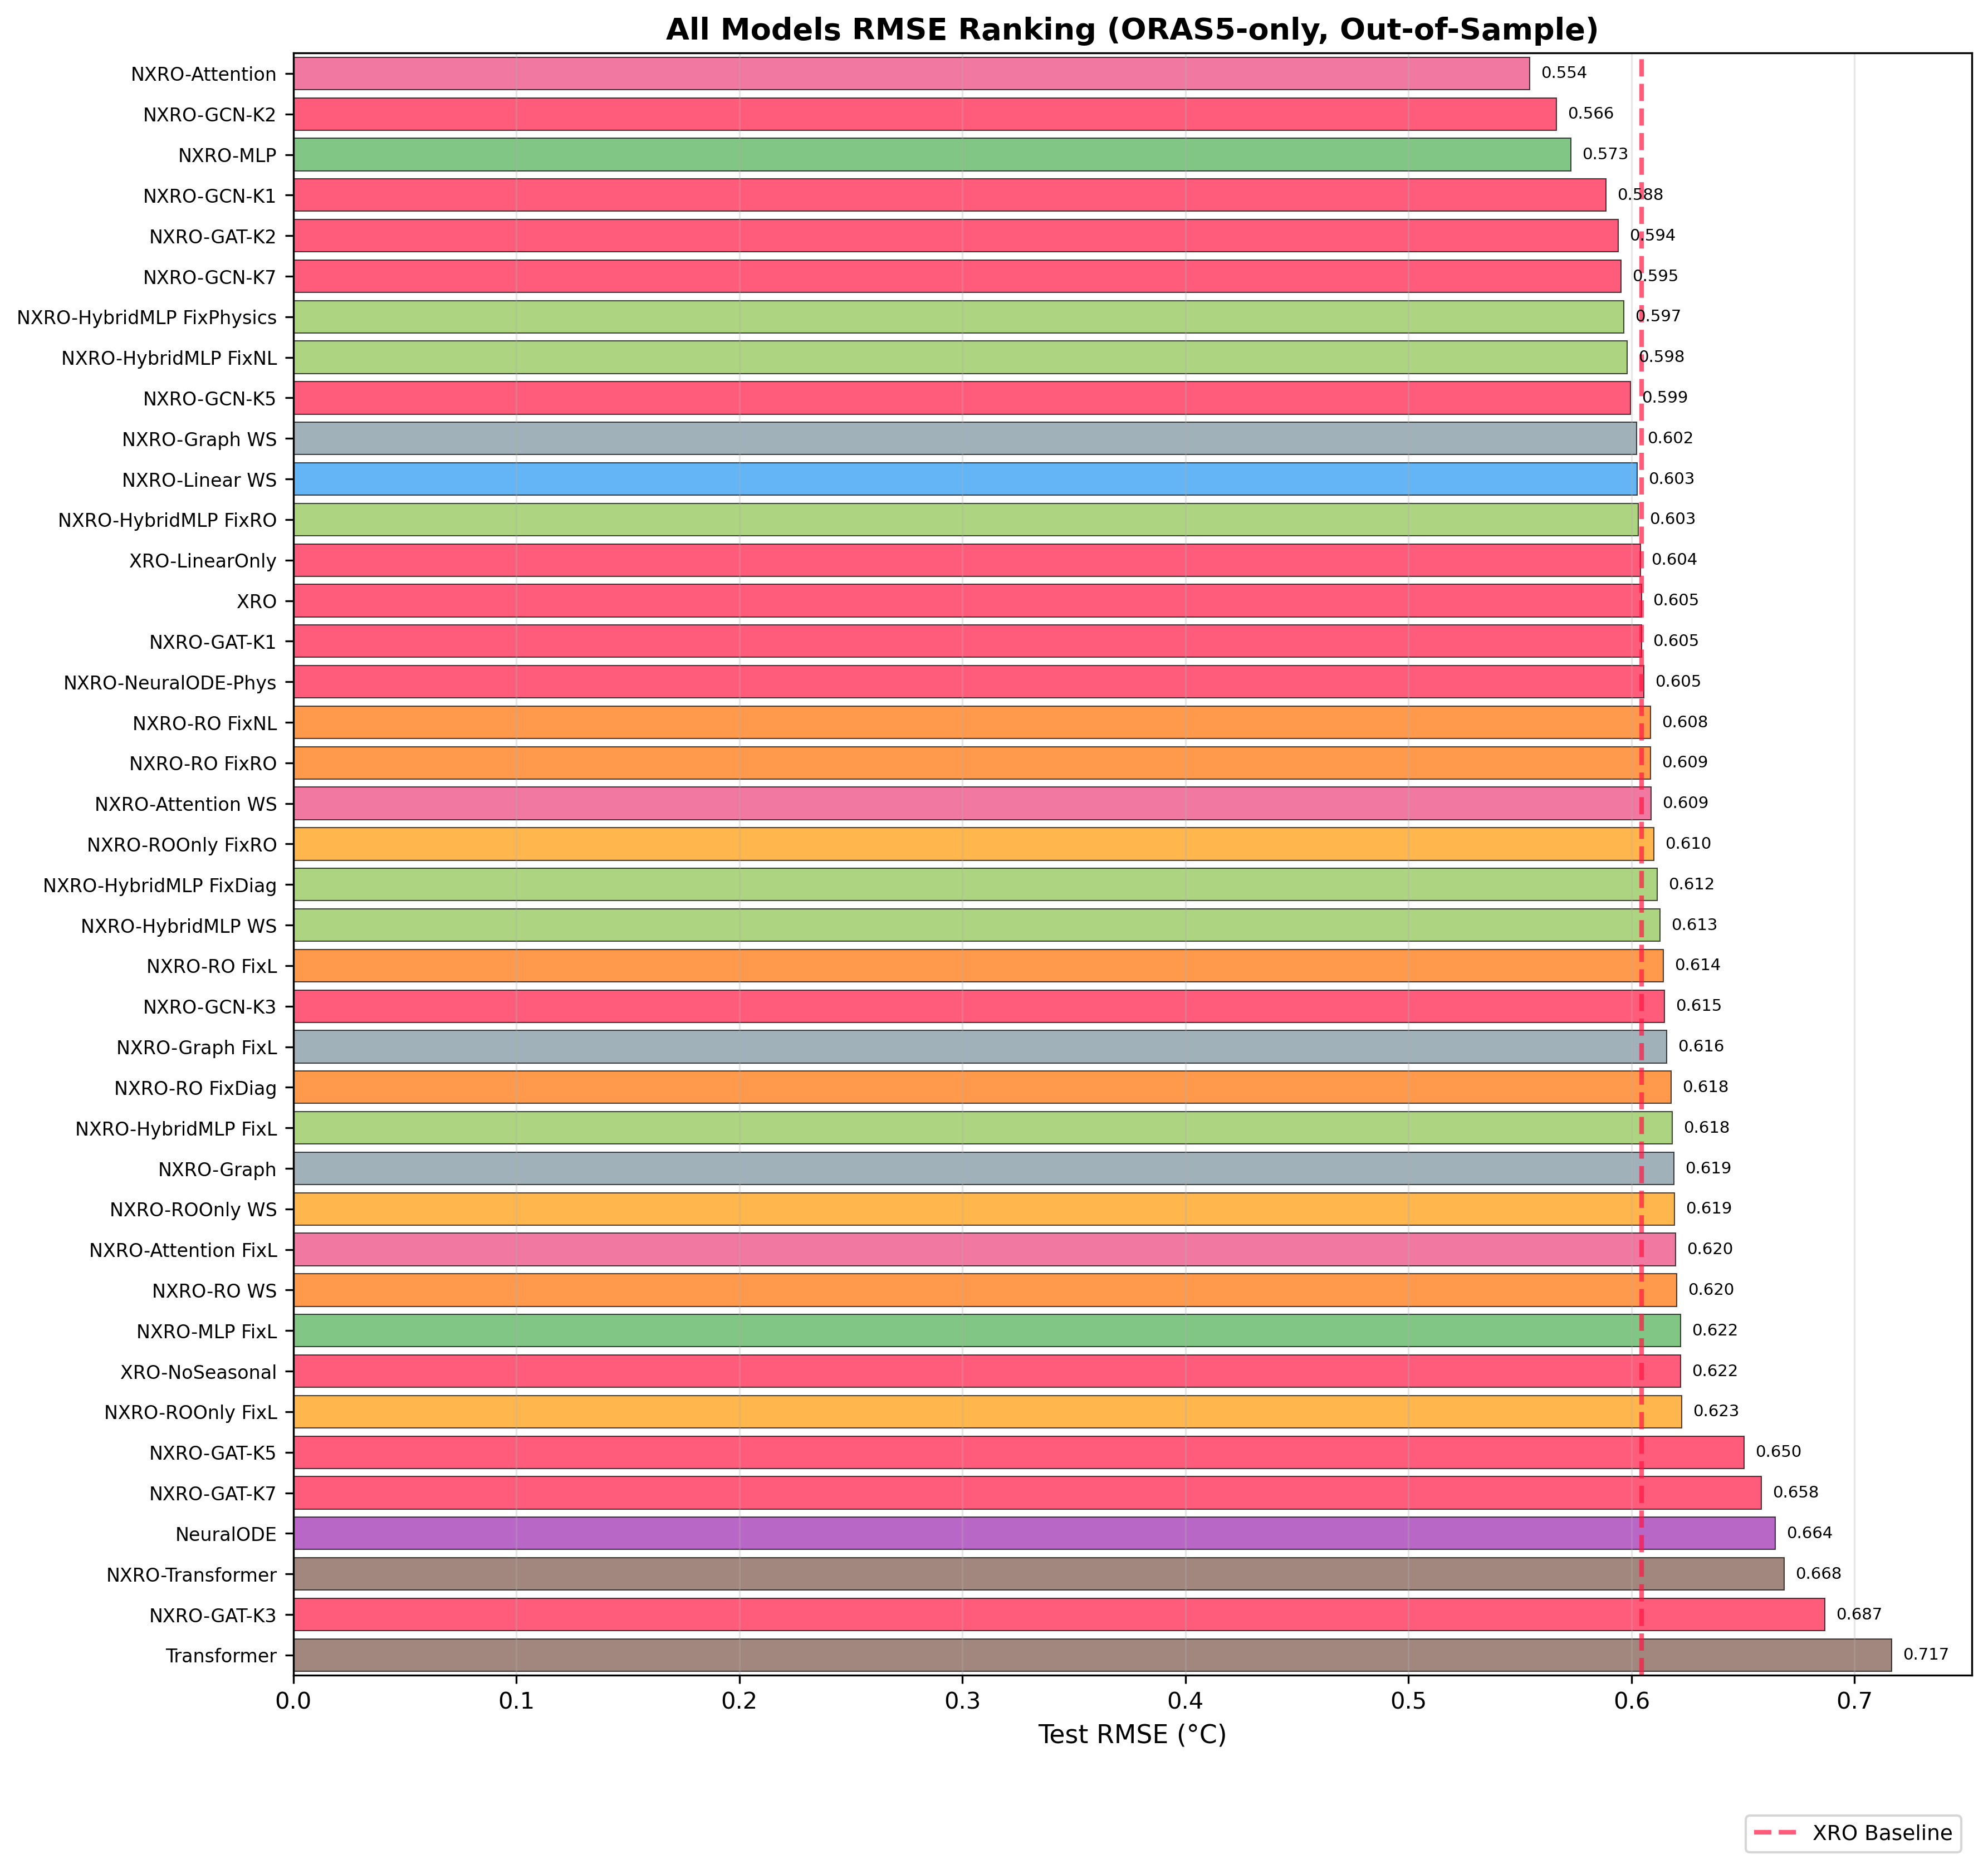
\includegraphics[width=0.9\linewidth]{figures/1_all_models_rmse_ranking.png}
    \caption{Comprehensive rankings for all models in the neural architecture search. About 18 models achieve better average RMSE results than the baseline model of XRO, with the best model to be the Neural XRO with MLP residual component.}
    \label{fig:all_models_rmse_ranking}
\end{figure}


\subsection{Complete End-to-End Results with Climate Simulation Data}

We present additional results for NXRO models trained using the CESM dataset pretraining + ORAS5 dataset finetuning set up. In this case, we only focus on the subset of NXRO models that do not use any warm-starts or parameter freezings, and fix the hyperparameter of NXRO variants that use graph neural network to only use the best hyperparameter found in the stage one setting. The results of the comprehensive RMSE result can be found in Figure \ref{fig:all_e2e_rmse_ranking}. The overall comprehensive ranking of all model variants (including both single stage training version and the end-to-end pretraining+finetuning version) can be found in Figure \ref{fig:all_rmse_ranking}, where the NXRO-MLP model still performs the best overall, despite its simplicity. 

\begin{figure}
    \centering
    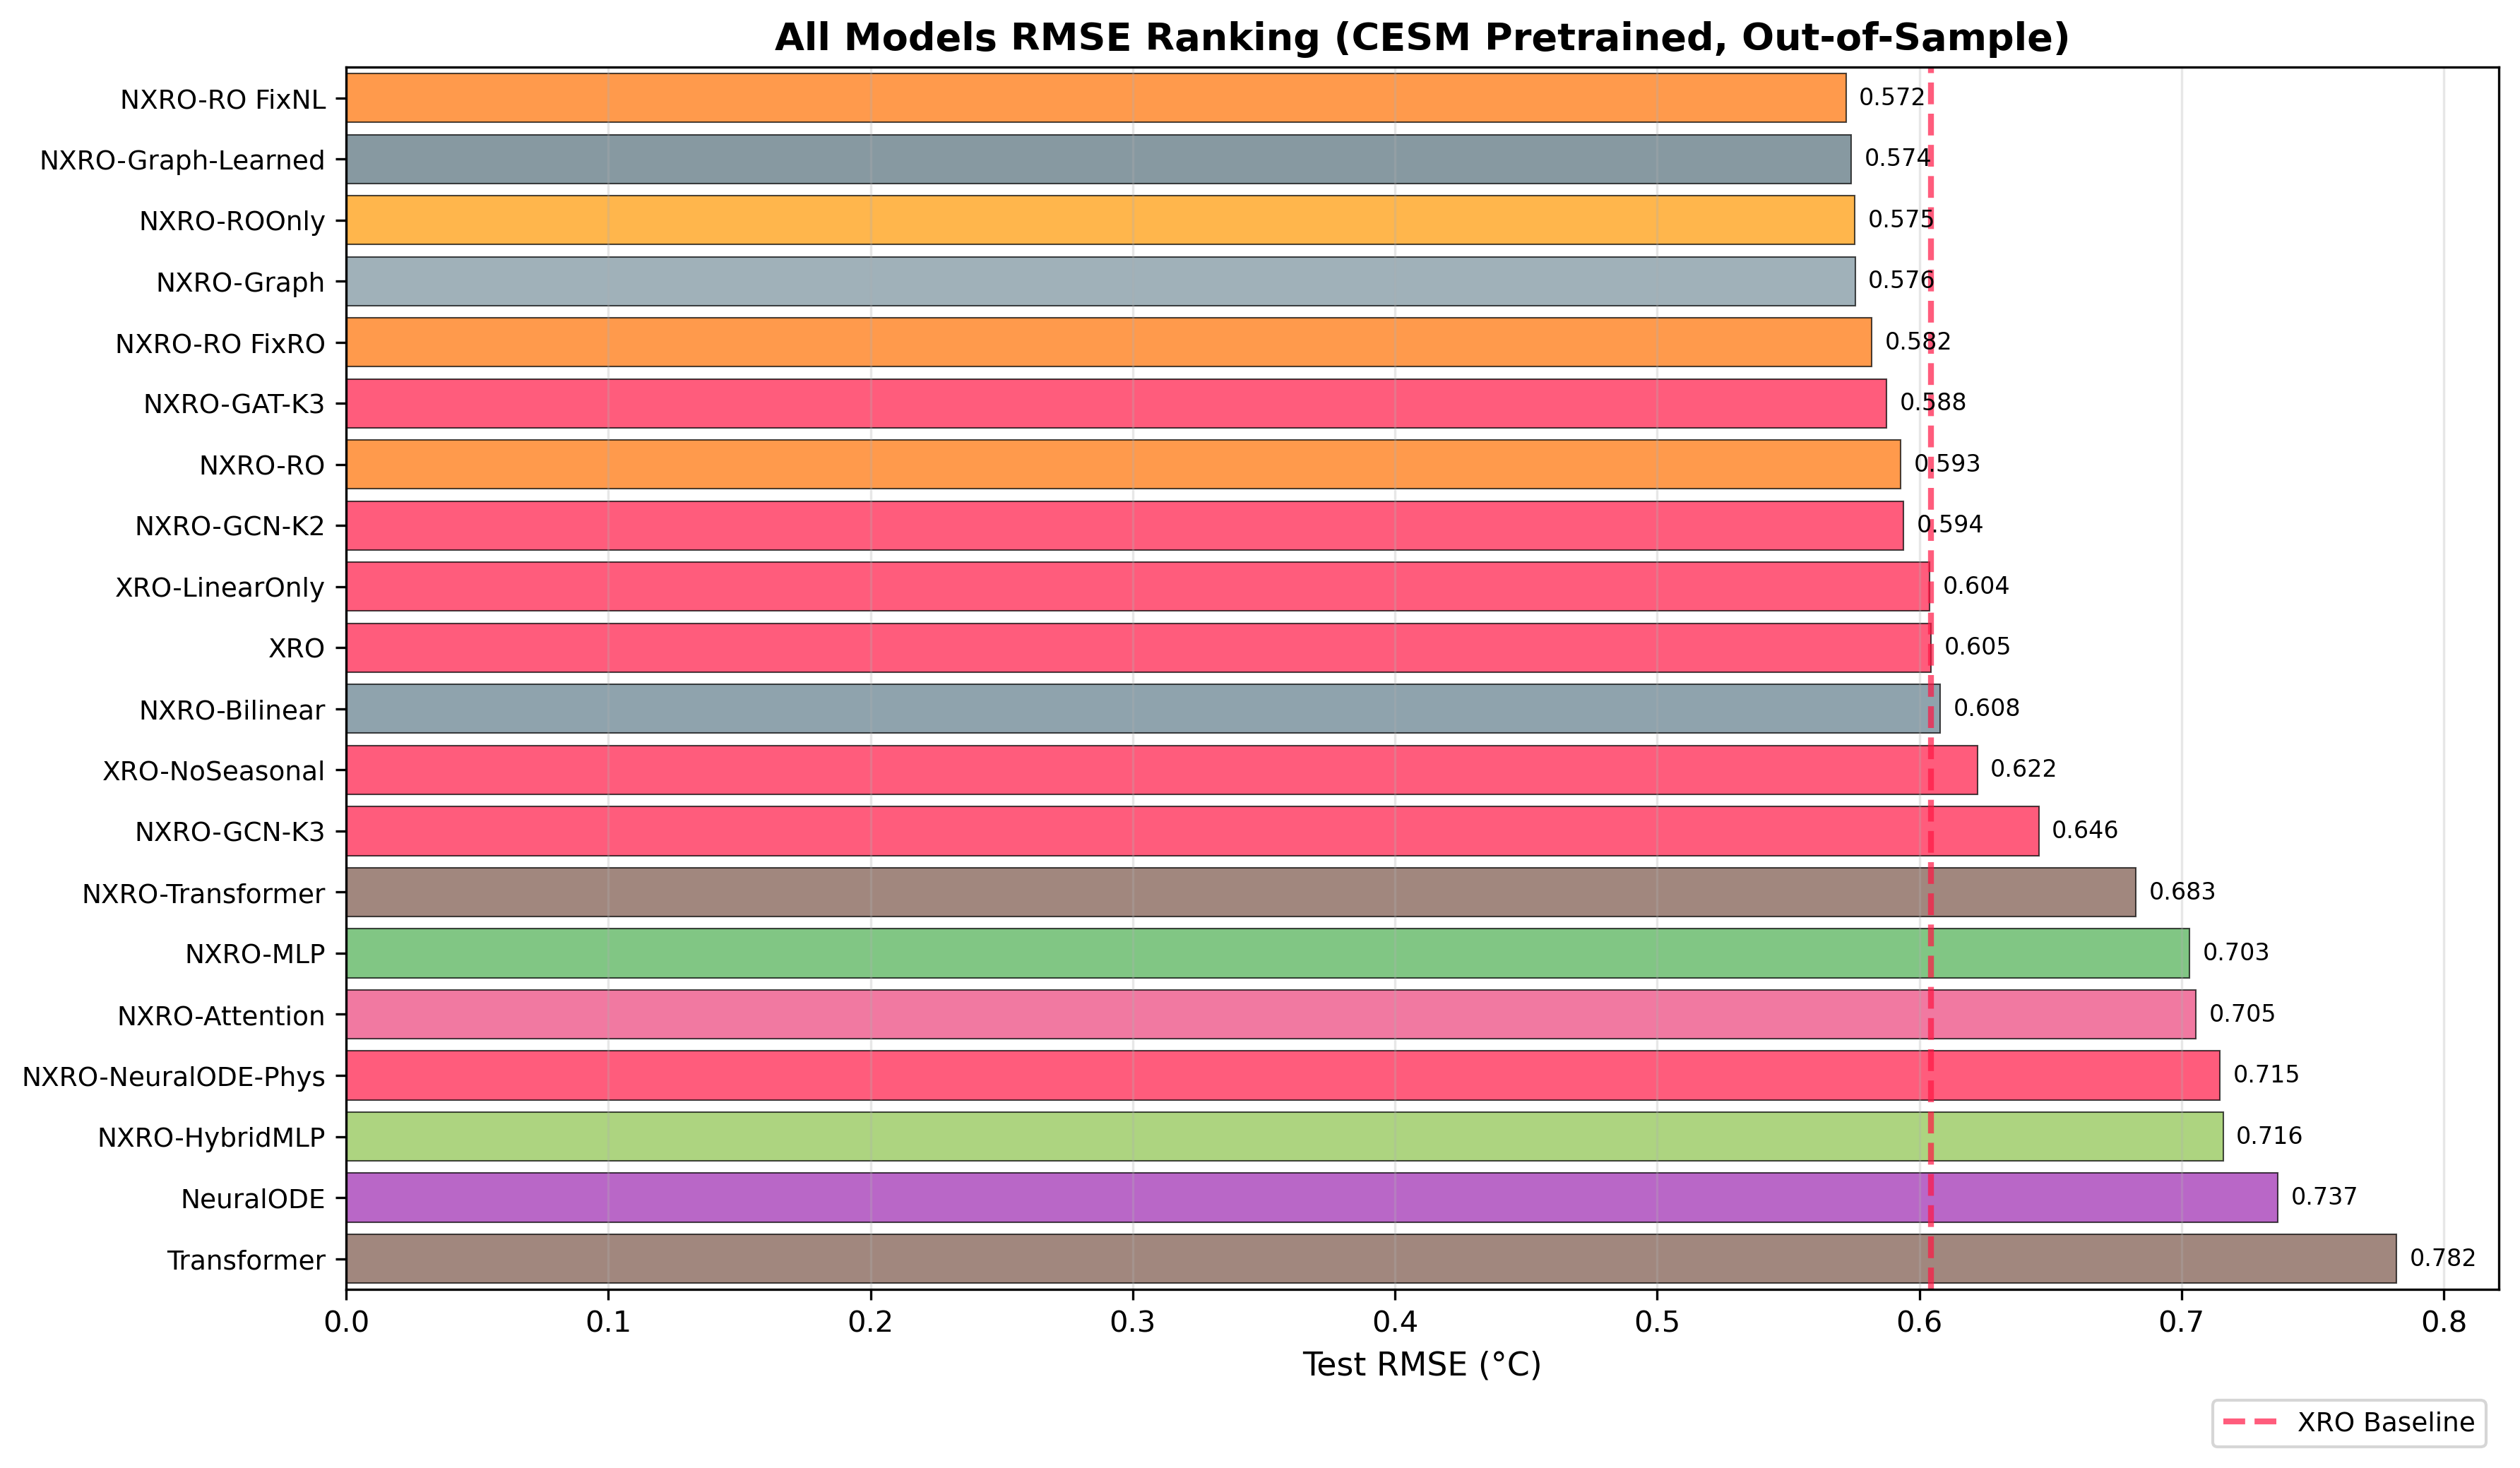
\includegraphics[width=\linewidth]{figures/2_all_models_rmse_ranking.png}
    \caption{The comprehensive results for all the selected NXRO variants, trained using the CESM-dataset training + ORAS5-dataset finetuning set up. It can be observed that the best performing models in the single-stage set up actually has degraded performance with the presence of more synthetic datasets, while many previously poor-performing models are improved.}
    \label{fig:all_e2e_rmse_ranking}
\end{figure}

\begin{figure}
    \centering
    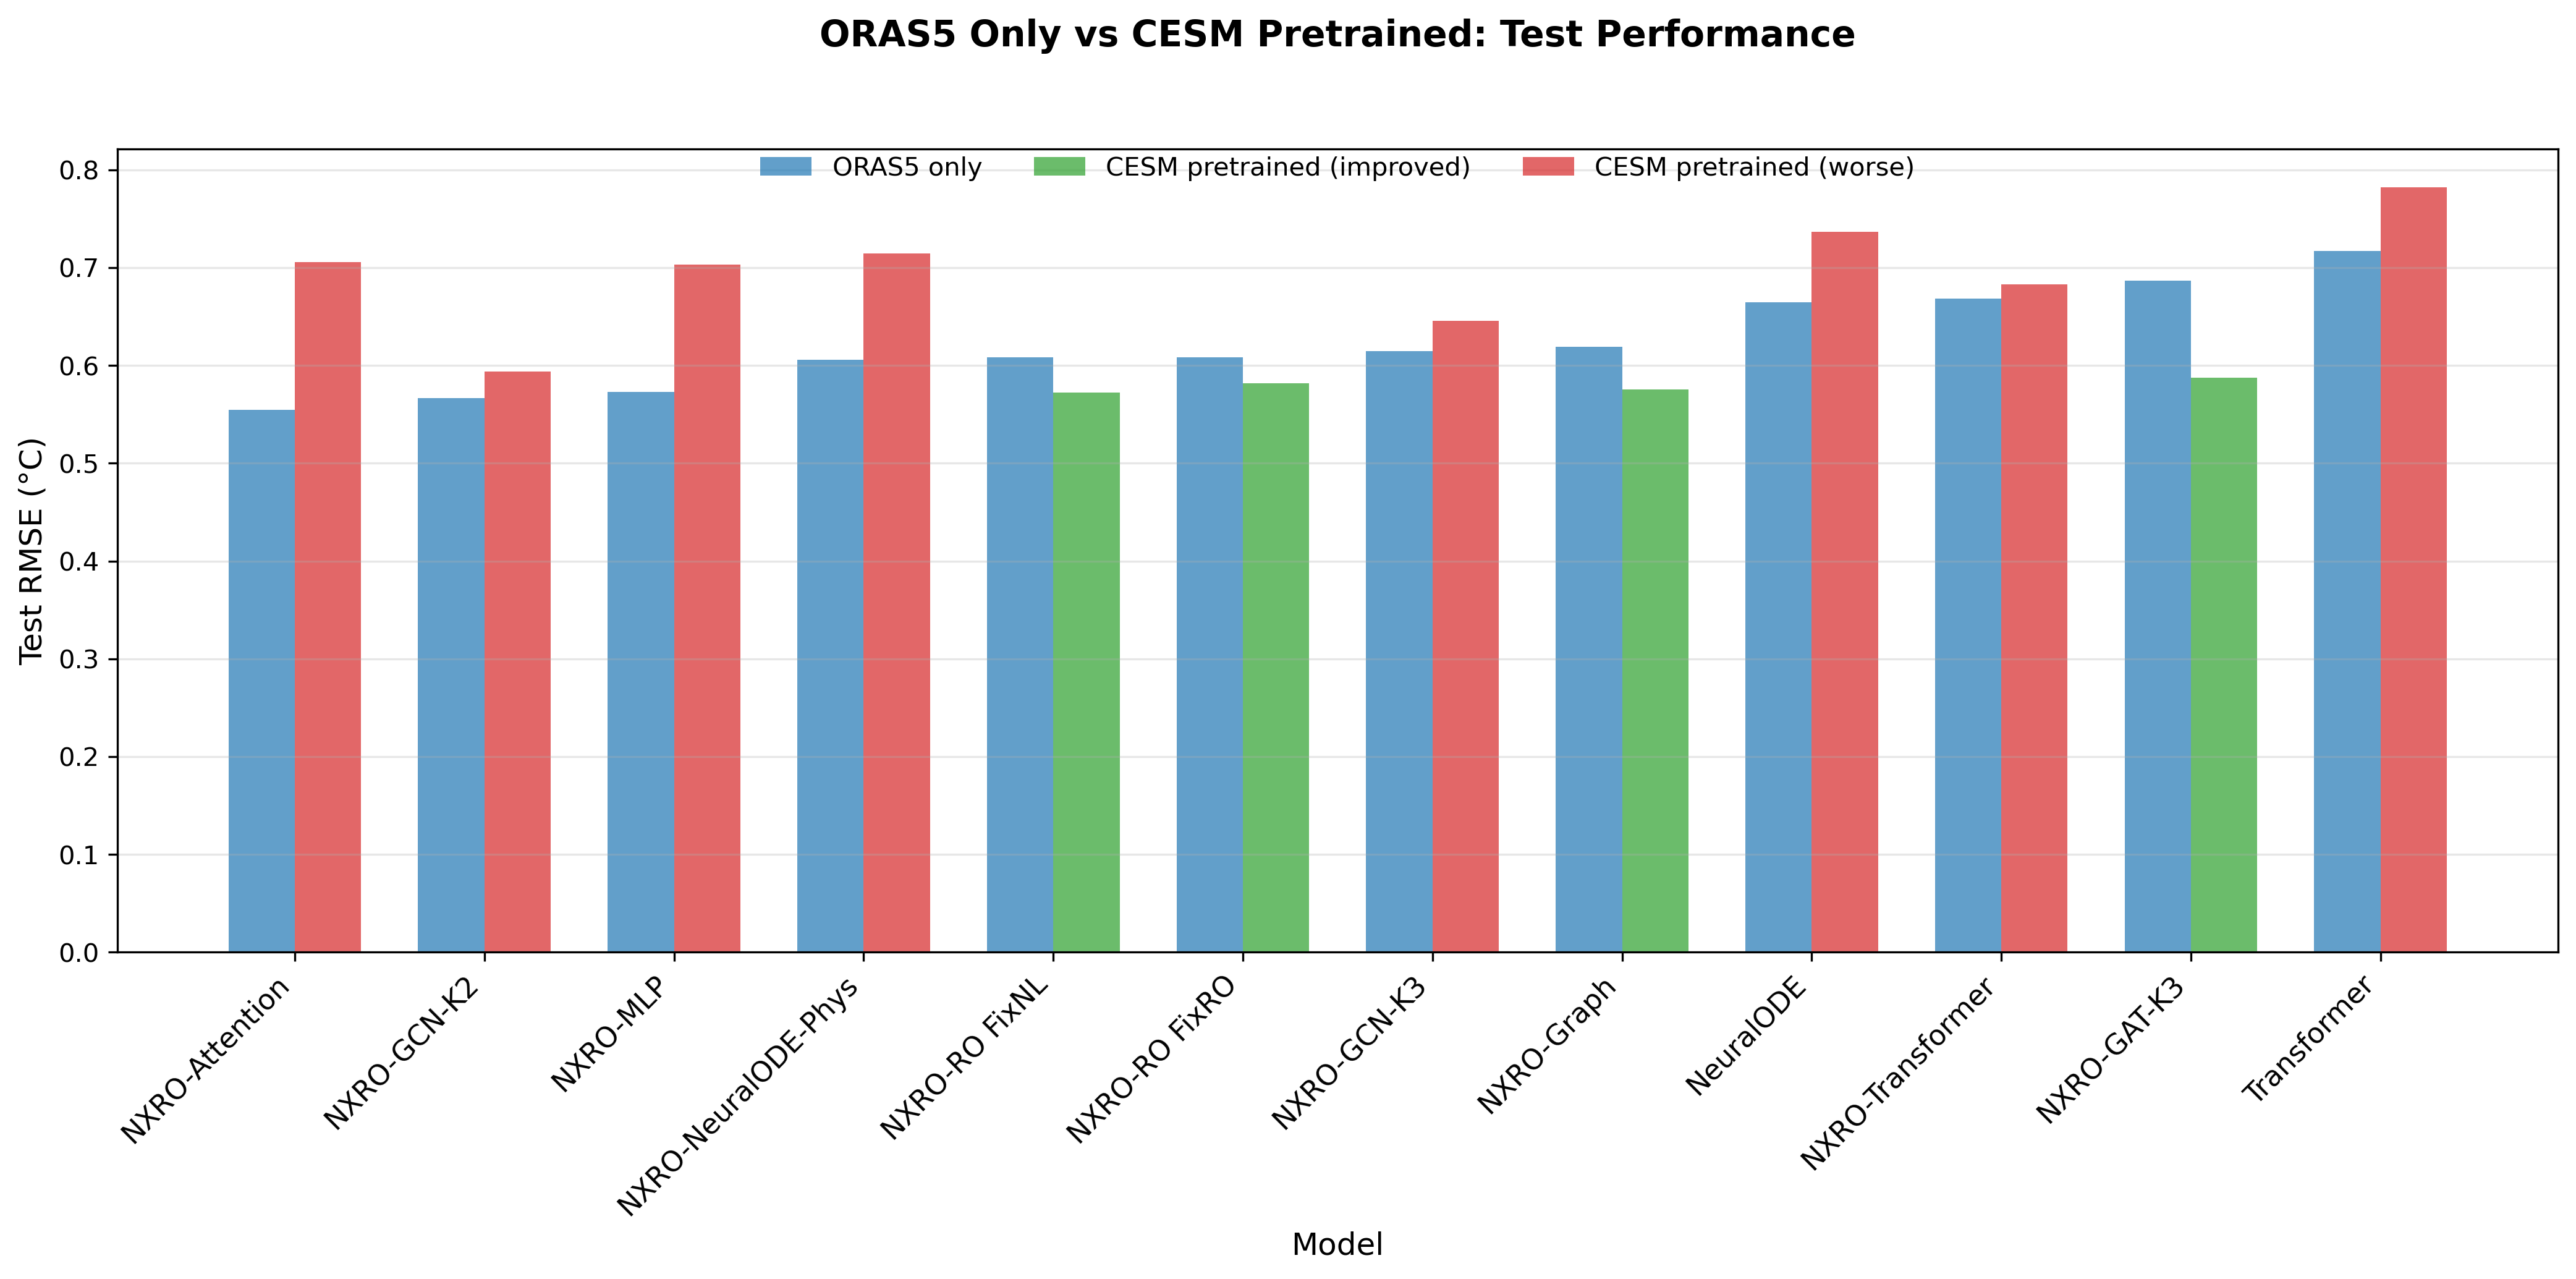
\includegraphics[width=\linewidth]{figures/6c_single_vs_two_stage_gap.png}
    \caption{Performance comparison of the same set of models with or without the pre-training step with the CESM climate simulation datasets.}
    \label{fig:one_vs_two}
\end{figure}

\begin{figure}
    \centering
    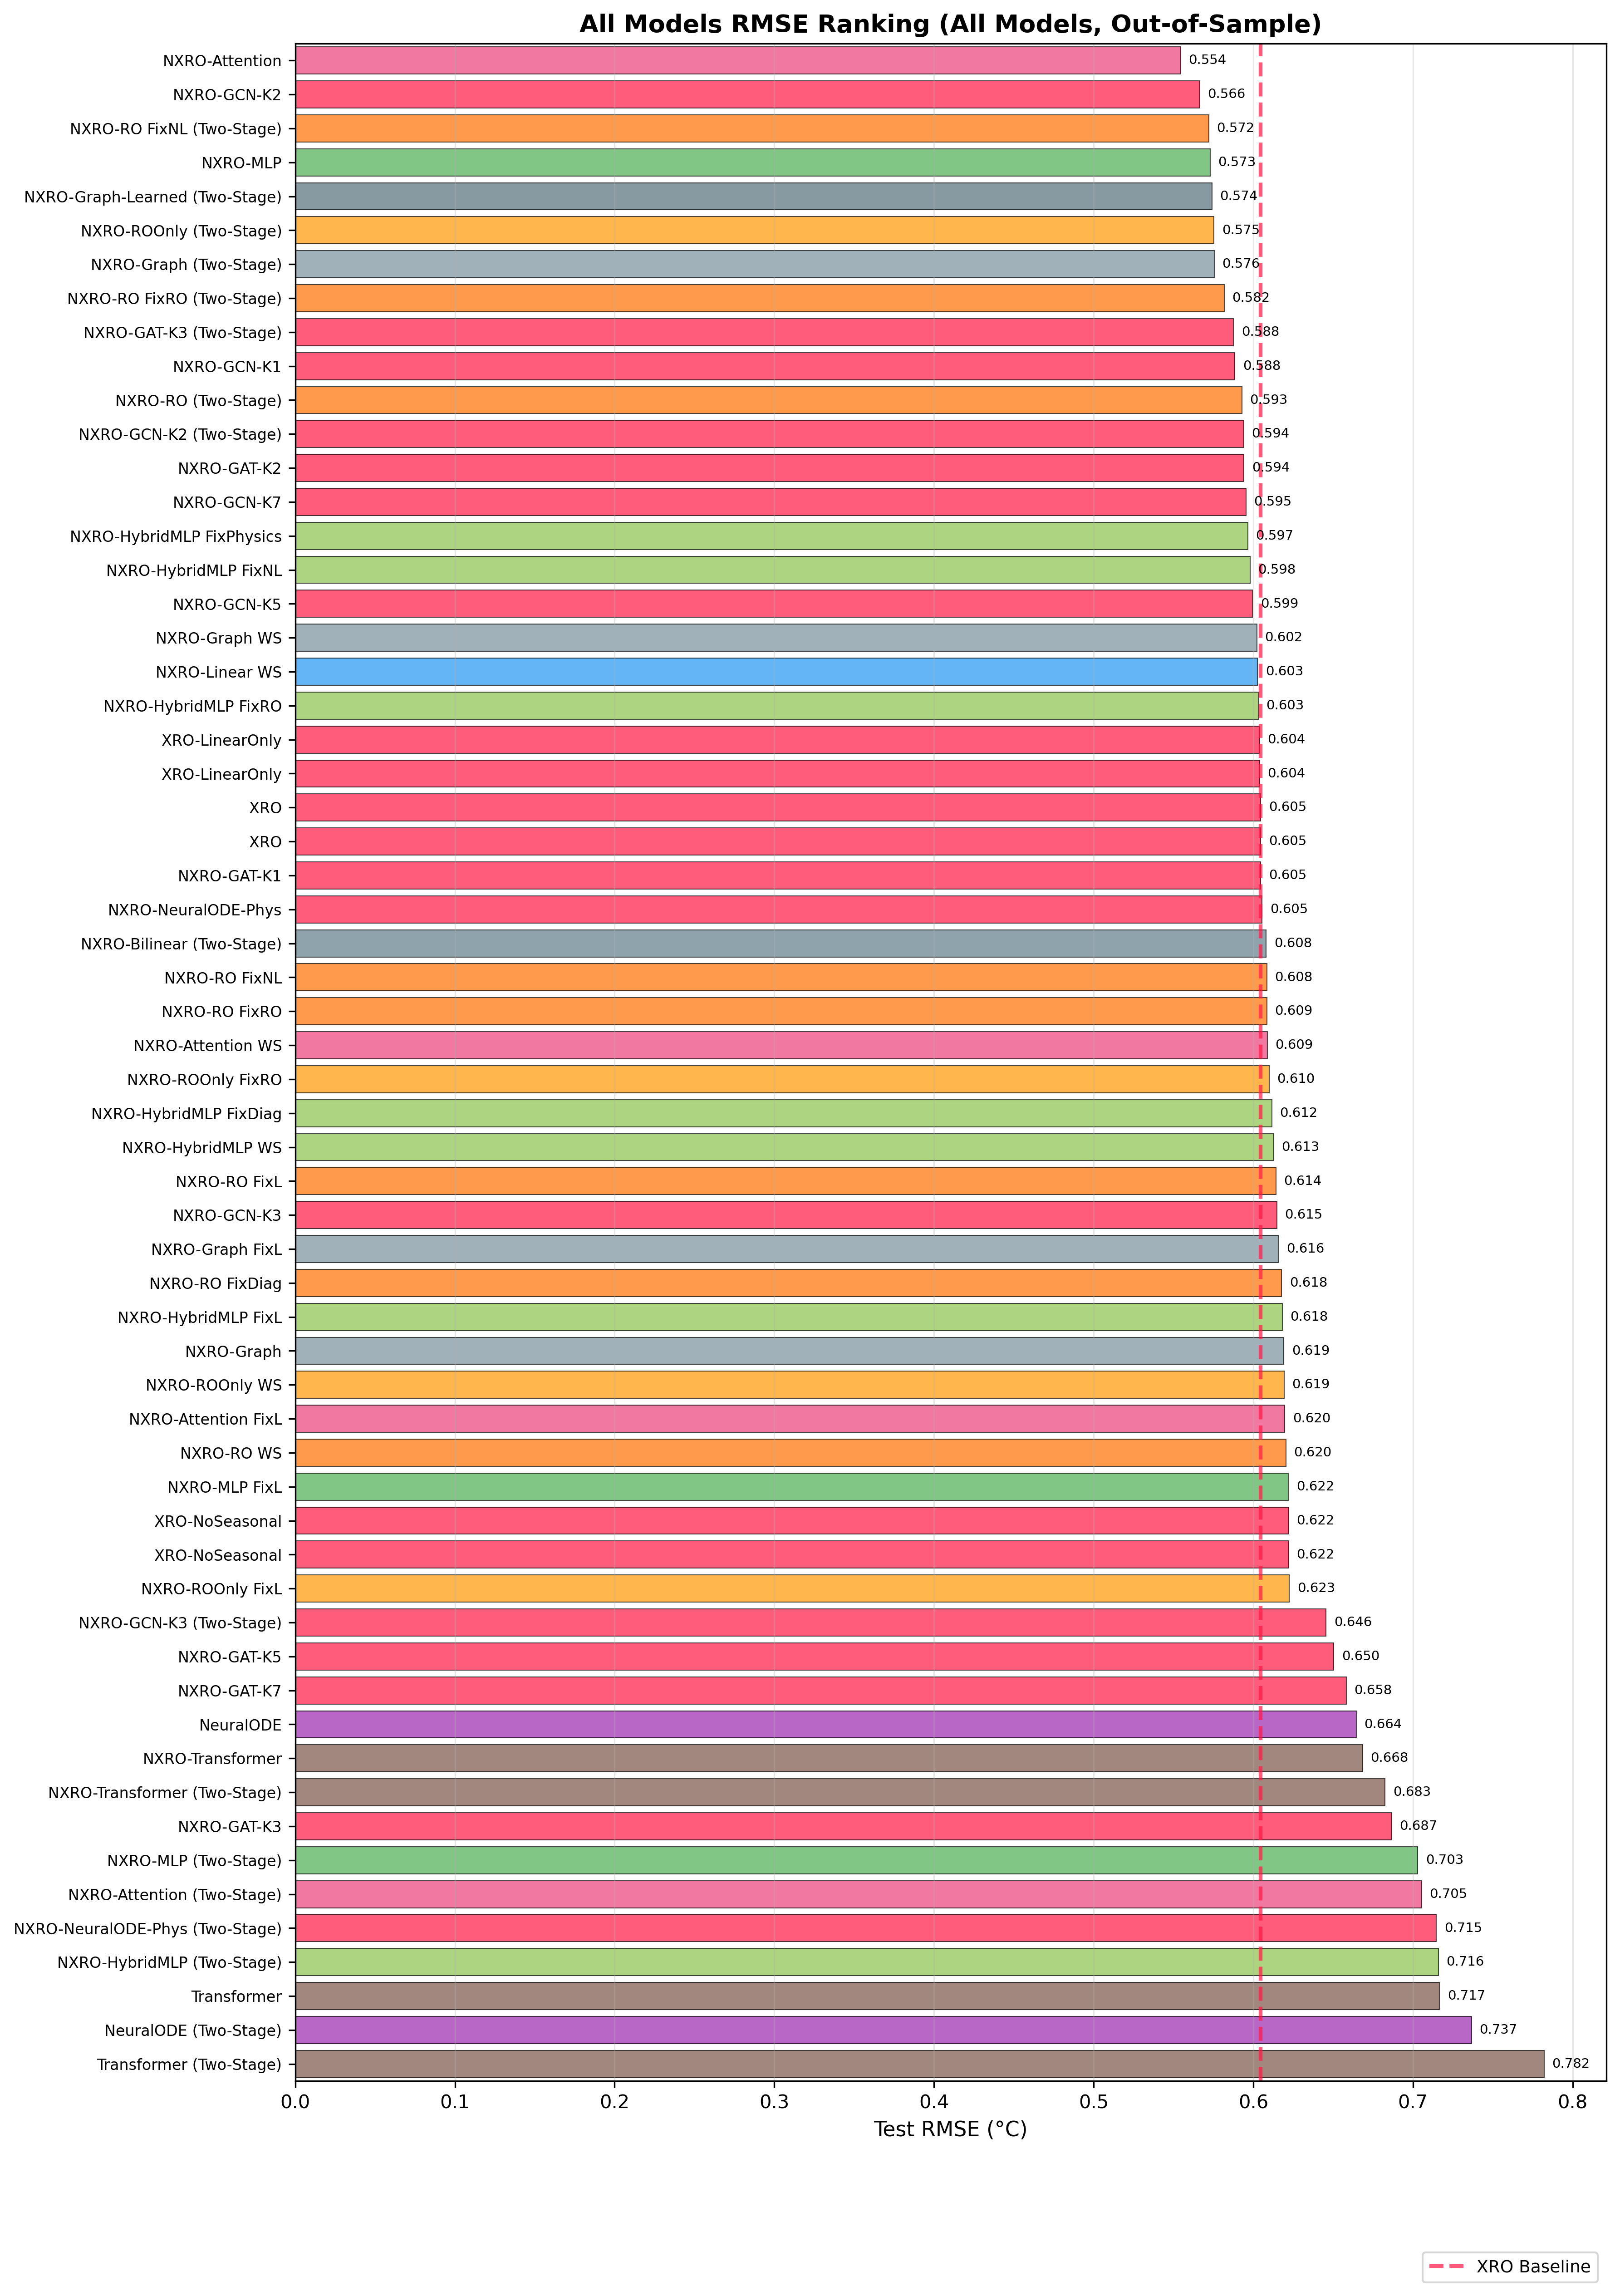
\includegraphics[width=0.9\linewidth]{figures/3_all_models_rmse_ranking.png}
    \caption{The overall ranking of all models, including both stage one-trained NXRO variants and NXRO variants trained using the CESM model simulation. Overall the NXRO-MLP model is still top-ranked.}
    \label{fig:all_rmse_ranking}
\end{figure}


The effect of pretraining on the CESM simulation dataset can be found in Figure \ref{fig:one_vs_two}. 



\subsection{ENSO Explainability with Graph Residual}

In this section, we present additional results by examining the learned KNN graph from the NXRO-Graph model. In the main paper, we have already presented the visualization of the learned adjacency matrix, the linear coupling strength between the climate indices, and the seasonal contribution from the nonlinear terms. Here we provide also \textbf{Seasonality Damping:} These are the diagonal elements $L_{ii}(t)$ of the coupling matrix across all 12 months. In this case, negative values indicate damped variable while positive values indicate amplification. The pattern shows that ENSO tends to be damped in Spring and peak in winter, which agrees with the observation. The results are in Figure \ref{fig:gcn_damping}. For completeness, we also show the statistics of the graph structure learned in the NXRO-GNN model in Figure \ref{fig:gcn_hubs}

\begin{figure}
    \centering
    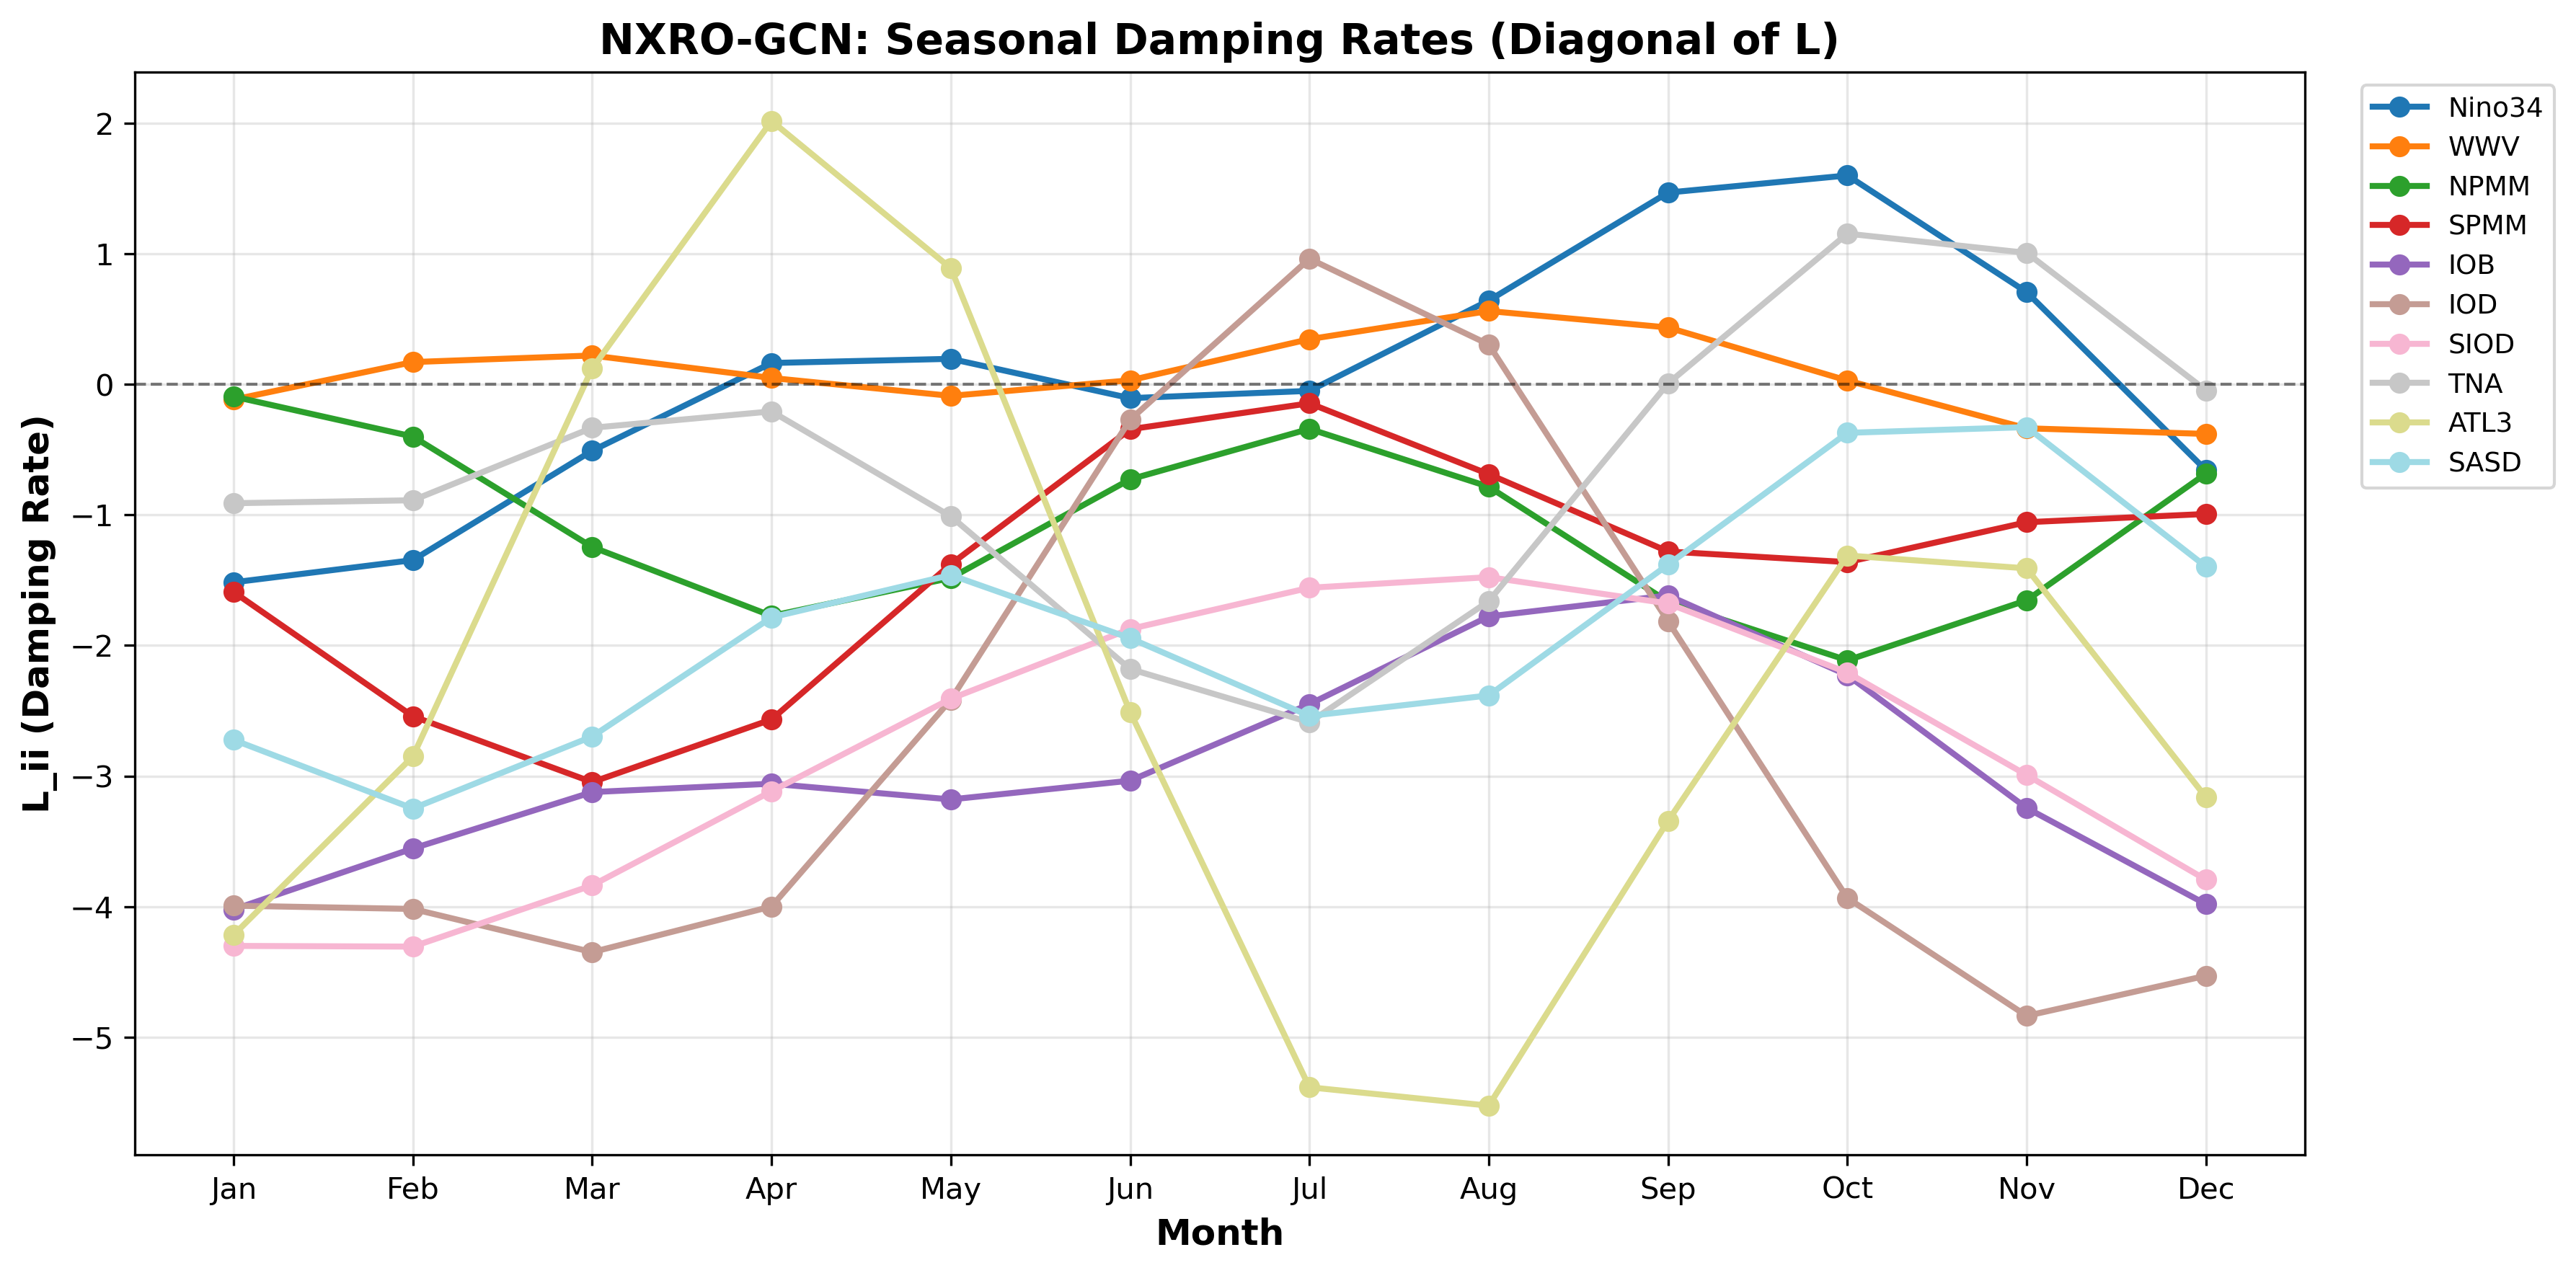
\includegraphics[width=\linewidth]{figures/gcn_damping_rates.png}
    \caption{Seasonality Damping coefficients of learned NXRO-GCN model. This shows the model learned damping factor for each index across different months.}
    \label{fig:gcn_damping}
\end{figure}


\begin{figure}
    \centering
    
\includegraphics[width=\linewidth]{sections/connections_and_hubs.png}
    \caption{The connection and hubs from the learned graph using the NXRO-GNN model with a learnable graph structure.}
    \label{fig:gcn_hubs}
\end{figure}




% \subsection{ENSO Explainability with Attention Residual}




% \begin{figure}
%     \centering
%     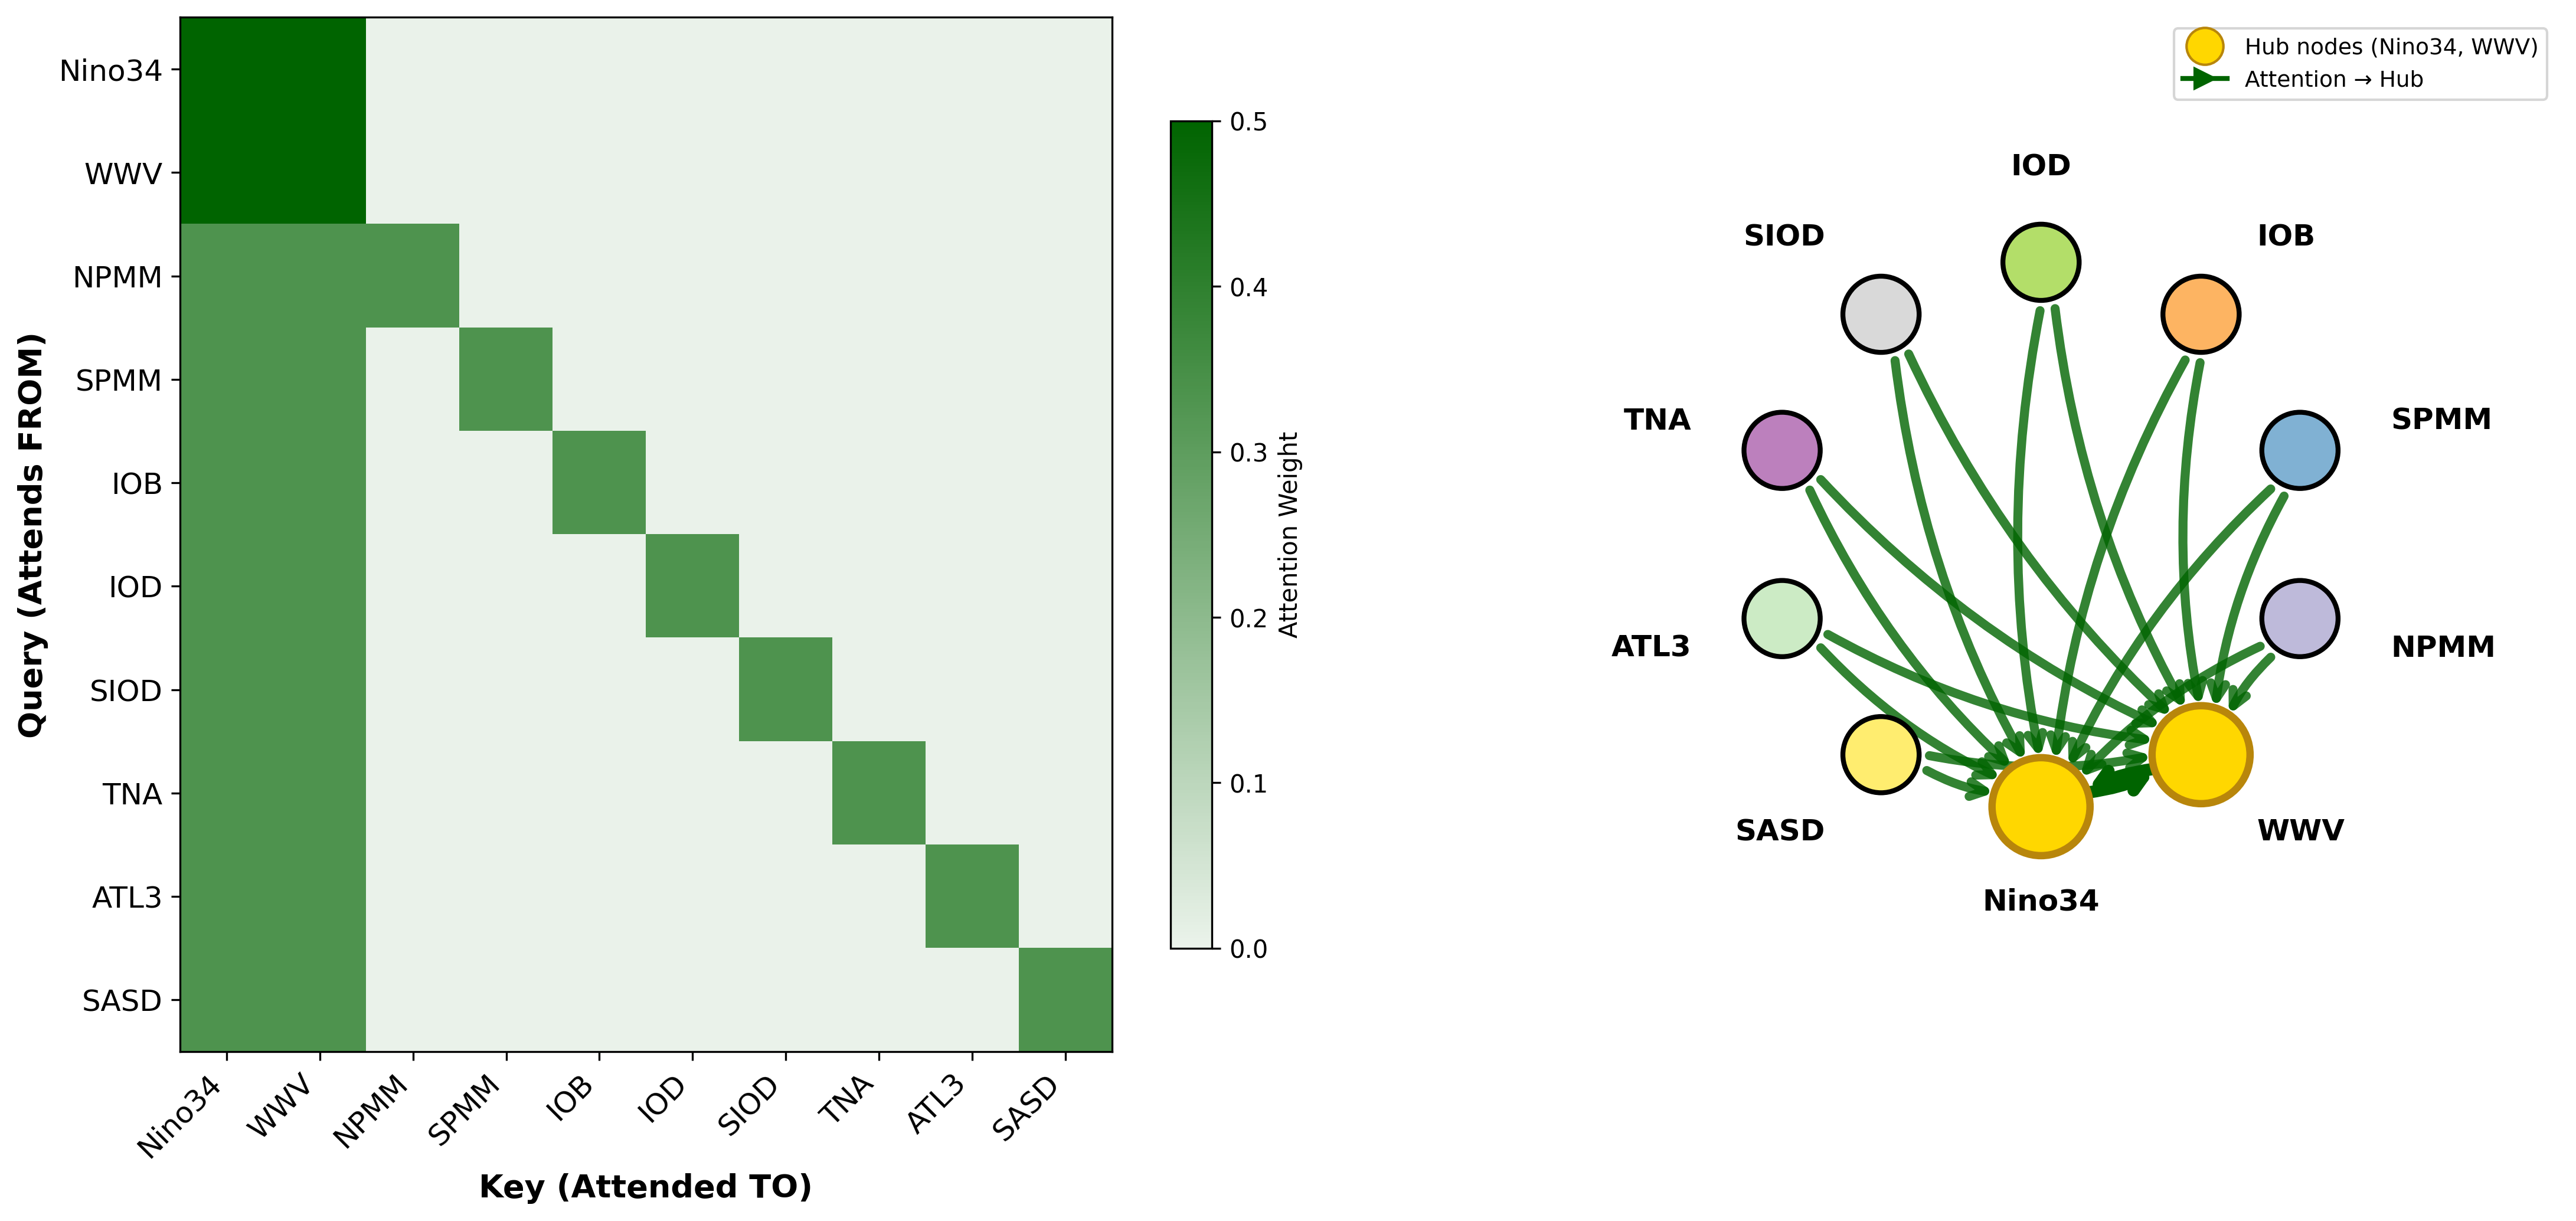
\includegraphics[width=\linewidth]{figures/attention_adjacency_and_network.png}
%     \caption{NXRO-Attention learned attention masking for interaction between components.}
%     \label{fig:attn_network}
% \end{figure}


% \begin{figure}
%     \centering
%     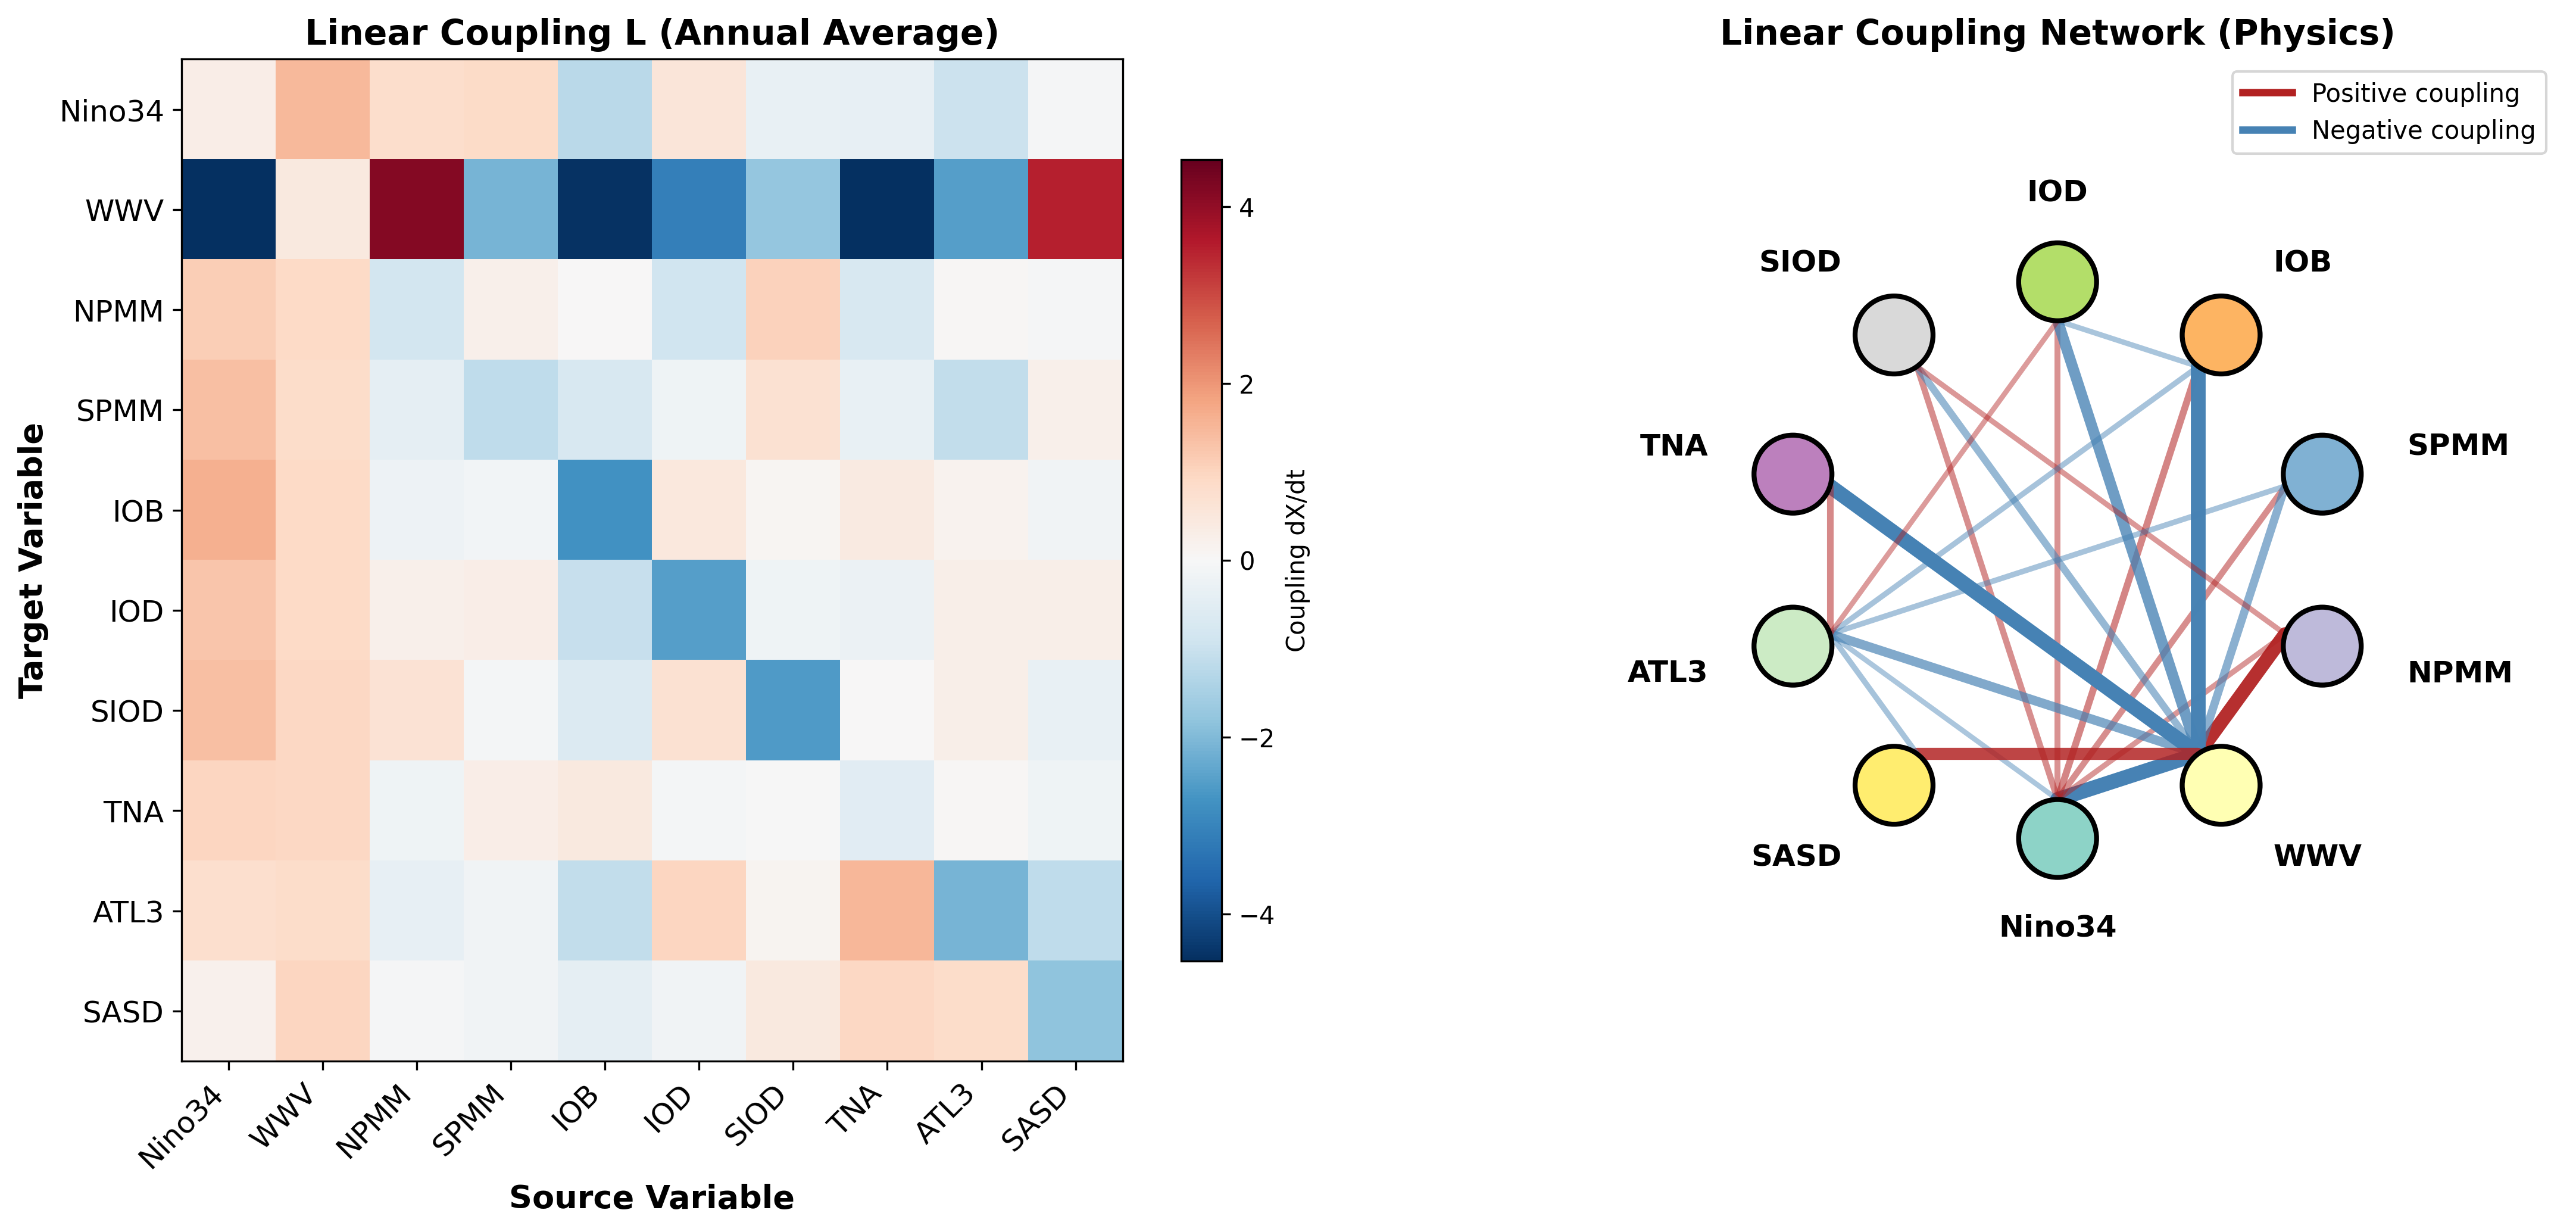
\includegraphics[width=\linewidth]{figures/attention_linear_coupling_L.png}
%     \caption{XNRO-Attention  model's learned linear component, demonstrating the strength of linear interaction strength between the climate modes.}
%     \label{fig:attn_linear}
% \end{figure}


% \begin{figure}
%     \centering
%     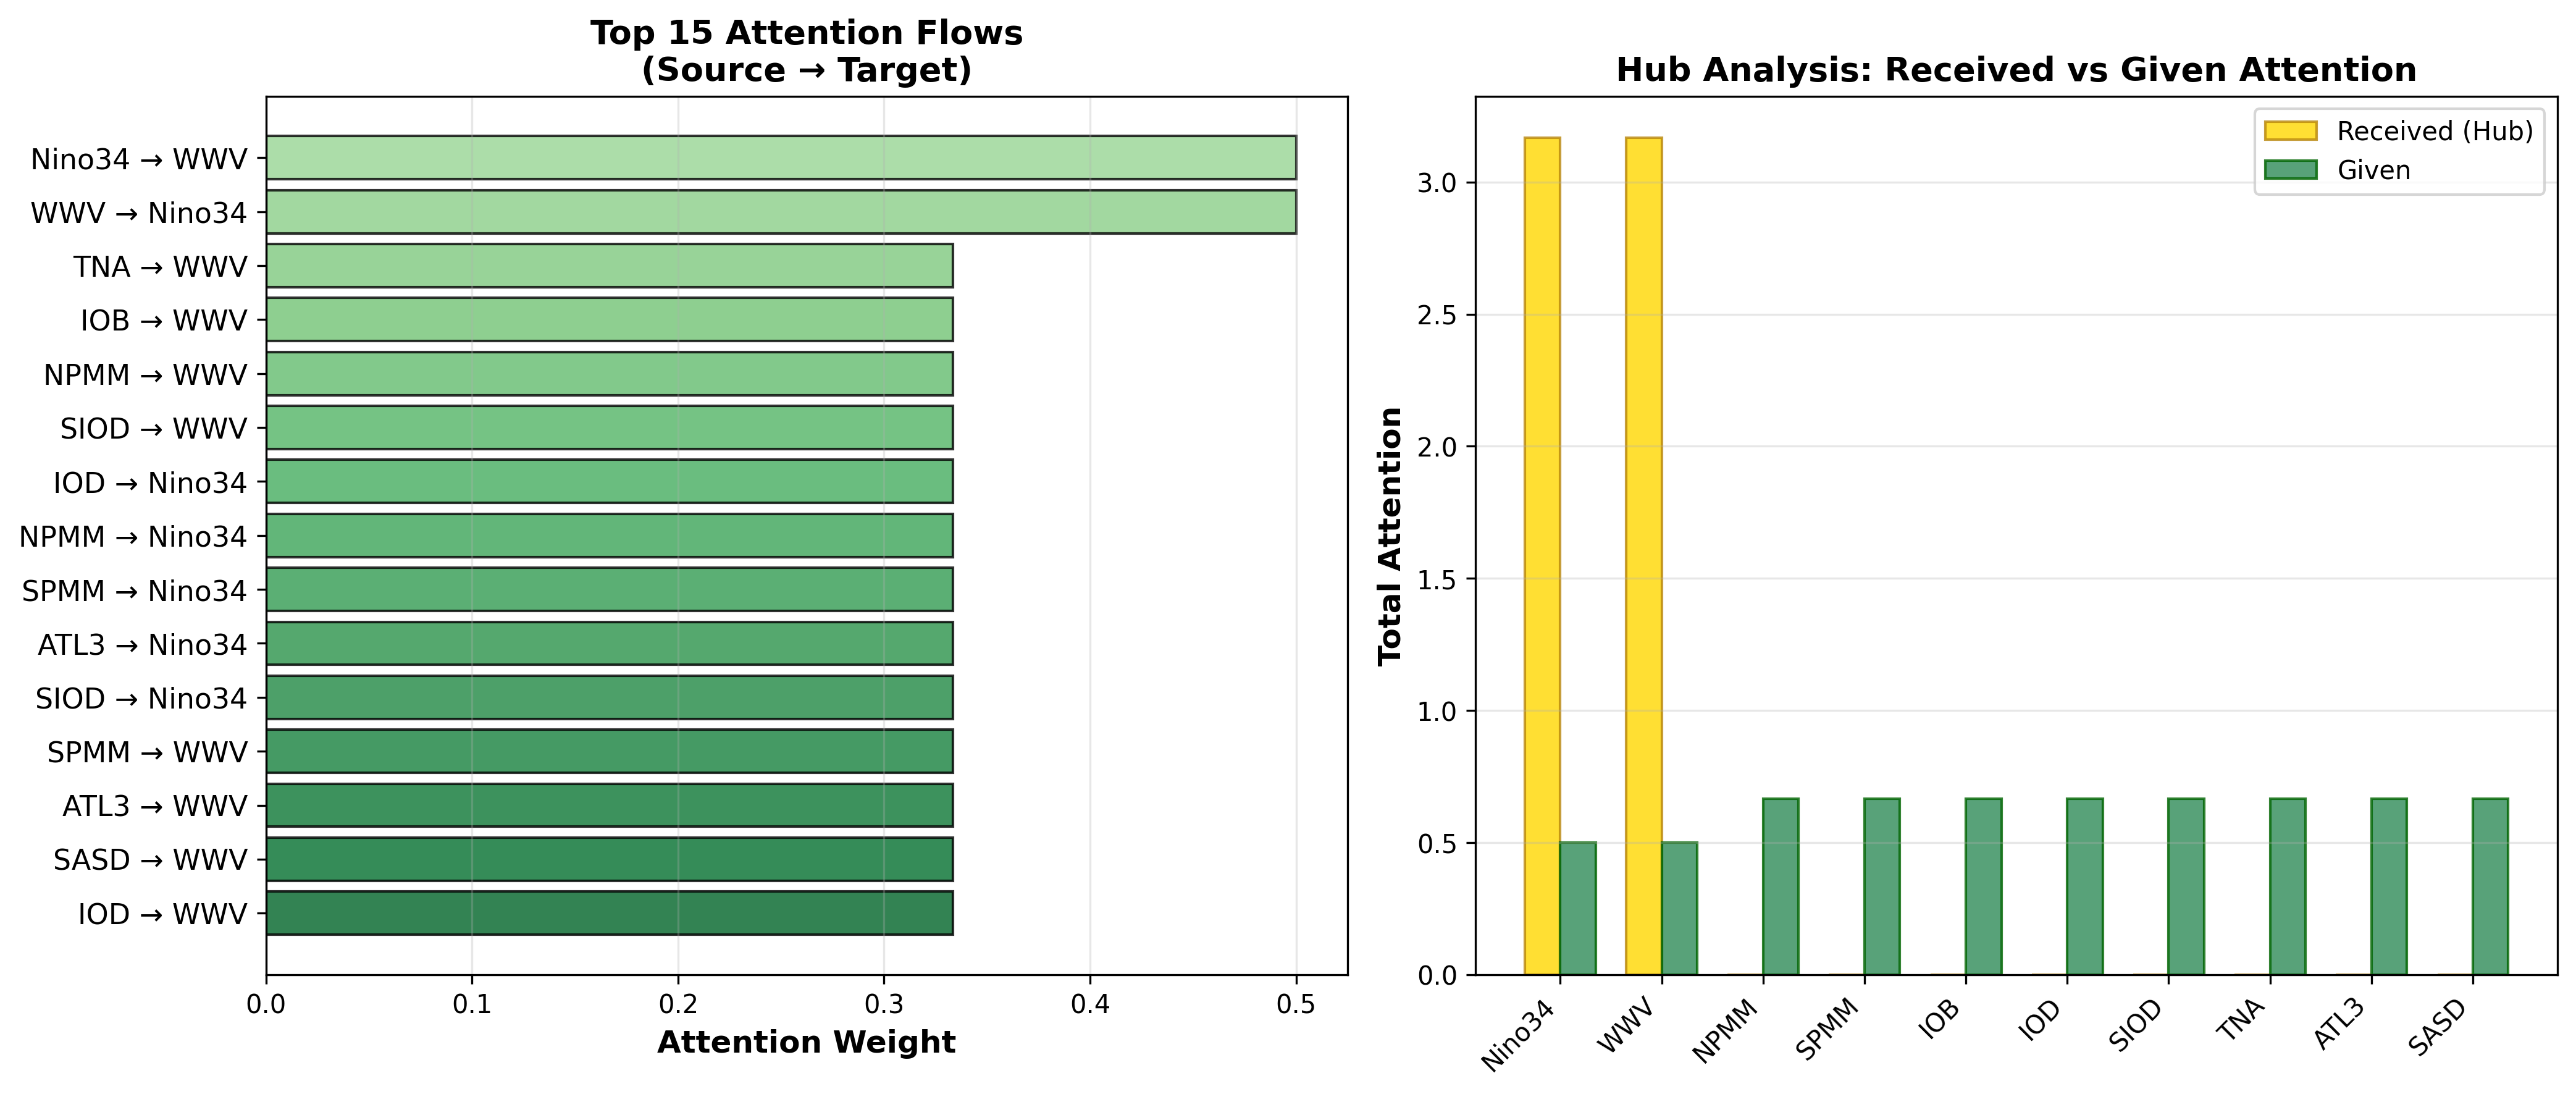
\includegraphics[width=\linewidth]{figures/attention_connections_and_hubs.png}
%     \caption{The connection and hubs from the learned NXRO-Attention model with learnable attention masking.}
%     \label{fig:attn_hubs}
% \end{figure}



% \begin{figure}
%     \centering
%     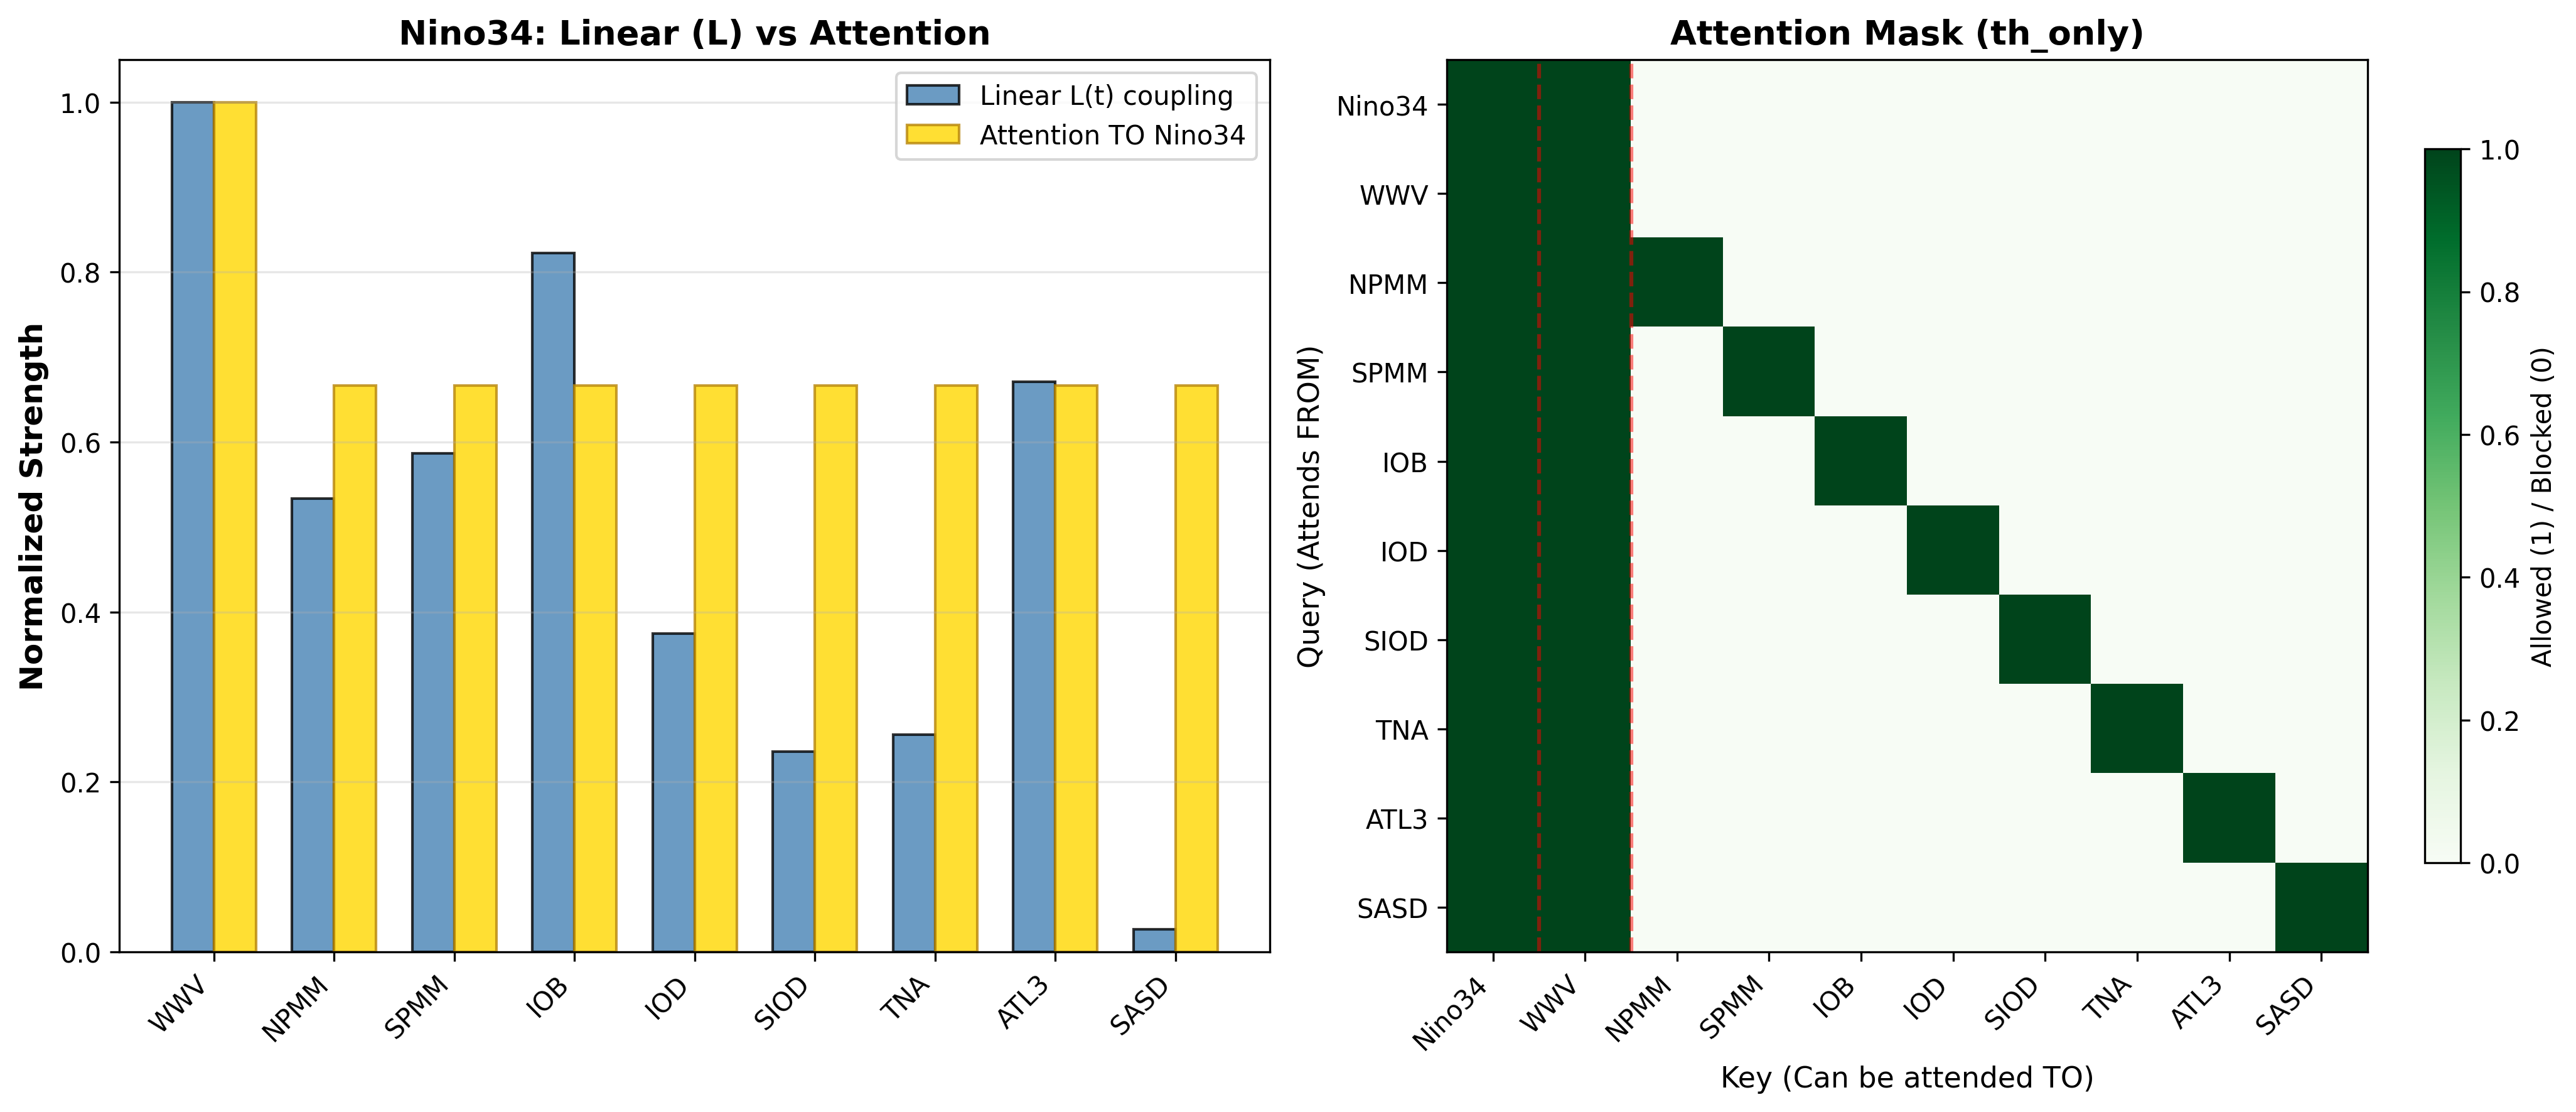
\includegraphics[width=\linewidth]{figures/linear_vs_attention.png}
%     \caption{The contribution from the linear and non-linear part of the NXRO-attention model.}
%     \label{fig:attn_linear_vs_nonlinear}
% \end{figure}



\section{Dataset Details} 
The definition of non-ENSO climate modes are detailed in Table \ref{tab:climate_modes}. We train our model based on reanalysis data from ECMWF Ocean Reanalysis System 5 (ORAS5). The monthly sea surface temperature anomalies (SSTA) are computed by subtracting the 1979–2022 monthly climatology and then removing a quadratic trend fit over 1979–2023. 

\begin{table}[h!]
\setlength{\tabcolsep}{3pt}
\centering
\caption{Definitions of non-ENSO climate-mode indices used in this study.}
\label{tab:climate_modes}
\resizebox{\columnwidth}{!}{
\begin{tabular}{p{0.40\columnwidth} c p{0.55\columnwidth}}
\toprule
\textbf{Climate Mode} & \textbf{Acronym} & \textbf{Description} \\
\midrule

North Pacific Meridional Mode & NPMM &
SSTAs averaged over 160$^\circ$--120$^\circ$W, 10$^\circ$--25$^\circ$N. \\

South Pacific Meridional Mode & SPMM &
SSTAs averaged over 110$^\circ$--90$^\circ$W, 25$^\circ$--15$^\circ$S. \\

Indian Ocean Basin mode & IOB &
SSTAs averaged over 40$^\circ$--100$^\circ$E, 20$^\circ$S--20$^\circ$N. \\

Indian Ocean Dipole mode & IOD &
SSTAs averaged over 50$^\circ$--70$^\circ$E, 10$^\circ$S--10$^\circ$N minus those averaged over
90$^\circ$--110$^\circ$E, 10$^\circ$S--0$^\circ$N. \\

Southern Indian Ocean Dipole mode & SIOD &
SSTAs averaged over 65$^\circ$--85$^\circ$E, 25$^\circ$--10$^\circ$S minus those averaged over
90$^\circ$--120$^\circ$E, 30$^\circ$--10$^\circ$S. \\

Tropical North Atlantic variability & TNA &
SSTAs averaged over 55$^\circ$--15$^\circ$W, 5$^\circ$--25$^\circ$N. \\

Atlantic Ni\~no & ATL3 &
SSTAs averaged over 20$^\circ$W--0$^\circ$E, 3$^\circ$S--3$^\circ$N. \\

South Atlantic Subtropical Dipole & SASD &
SSTAs averaged over 60$^\circ$--0$^\circ$W, 45$^\circ$--35$^\circ$S minus those averaged over
40$^\circ$W--20$^\circ$E, 30$^\circ$--20$^\circ$S. \\
\bottomrule
\end{tabular}
}
\end{table}

To perform transfer-learning experiment, we utilize the output from a large ensemble of climate model simulations conducted with the Community Earth System Model (CESM), version 2 \cite{LENS}. Each member within the CESM large ensemble simulations uses nominal 1 degree horizontal resolution and is driven by the same observed changes in external influences (e.g., greenhouse gases and aerosols) that affected the real world over the historical period. Because the climate system is inherently chaotic, small differences in the initial state can grow over time and produce different climate, a phenomenon commonly called internal variability. To sample internal variability as comprehensively as possible, each ensemble member is conducted with the same external forcings and model configuration, but is initialized with a slight perturbation to the atmospheric temperature field. In total, 100 ensemble members are performed. 








\section{Additional Stochastic Forecast Visualizations}

In this section we provide additional visualization of the special ENSO events forecast:
\begin{enumerate}
    \item In Figure \ref{fig:full_stochastic_forecast} we present the stochastic forecast visualization for the entire validation period, using the stochastic ensemble at a lead time of 6 months for each time index.
    \item In Figure \ref{fig:1997_dev} through Figure \ref{fig:2011_lanina} we show the forecast of different models for several samples of notable ENSO events. 
\end{enumerate}

\begin{figure}
    \centering
    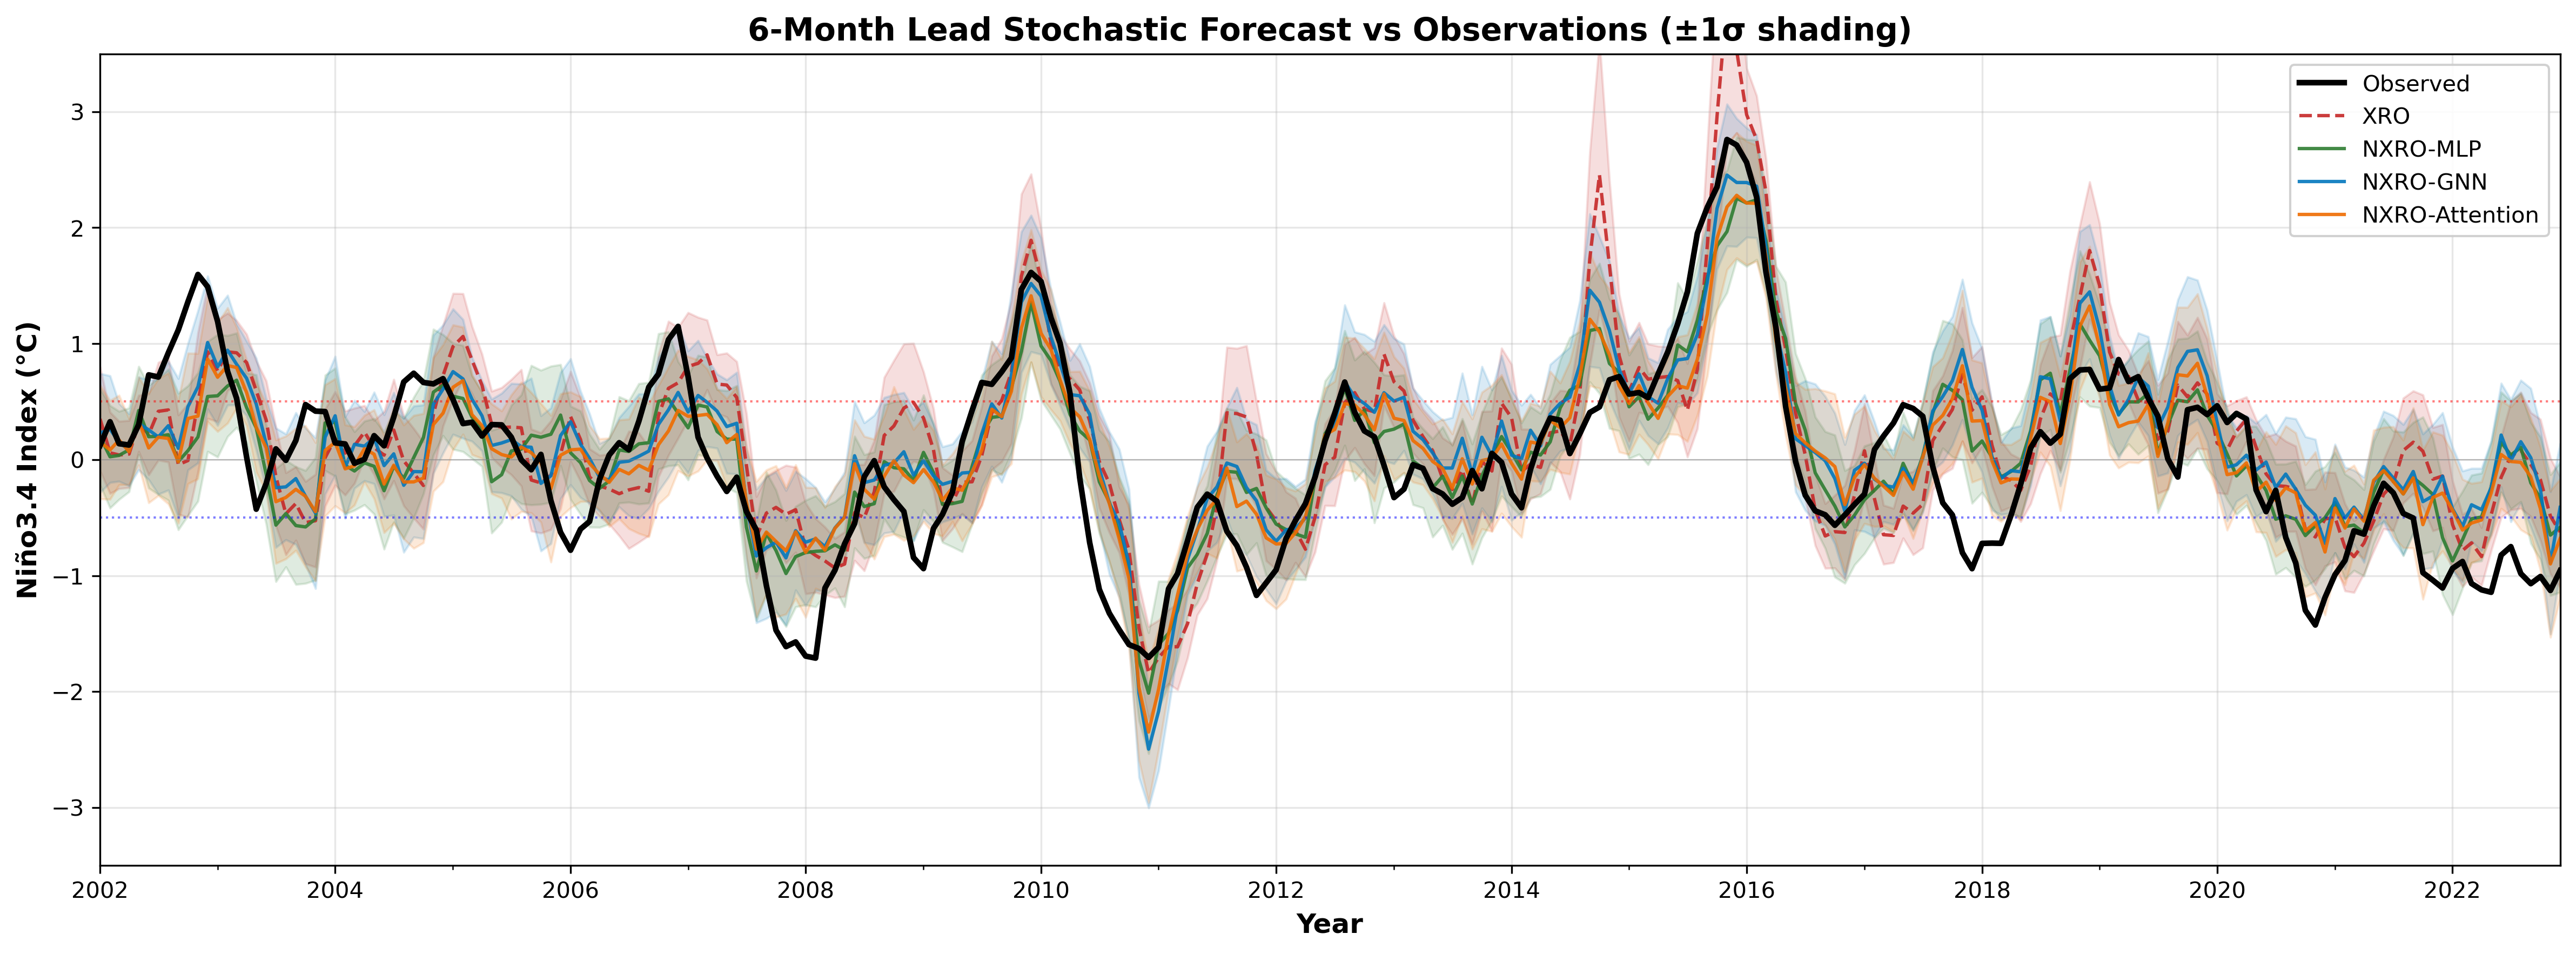
\includegraphics[width=\linewidth]{figures/1h_stochastic_forecast.png}
    \caption{The full stochastic forecast visualization using the ensemble prediction at the validation period. The plot is generated using 6-month forecast at each month.}
    \label{fig:full_stochastic_forecast}
\end{figure}


\begin{figure}[t]
  \centering
  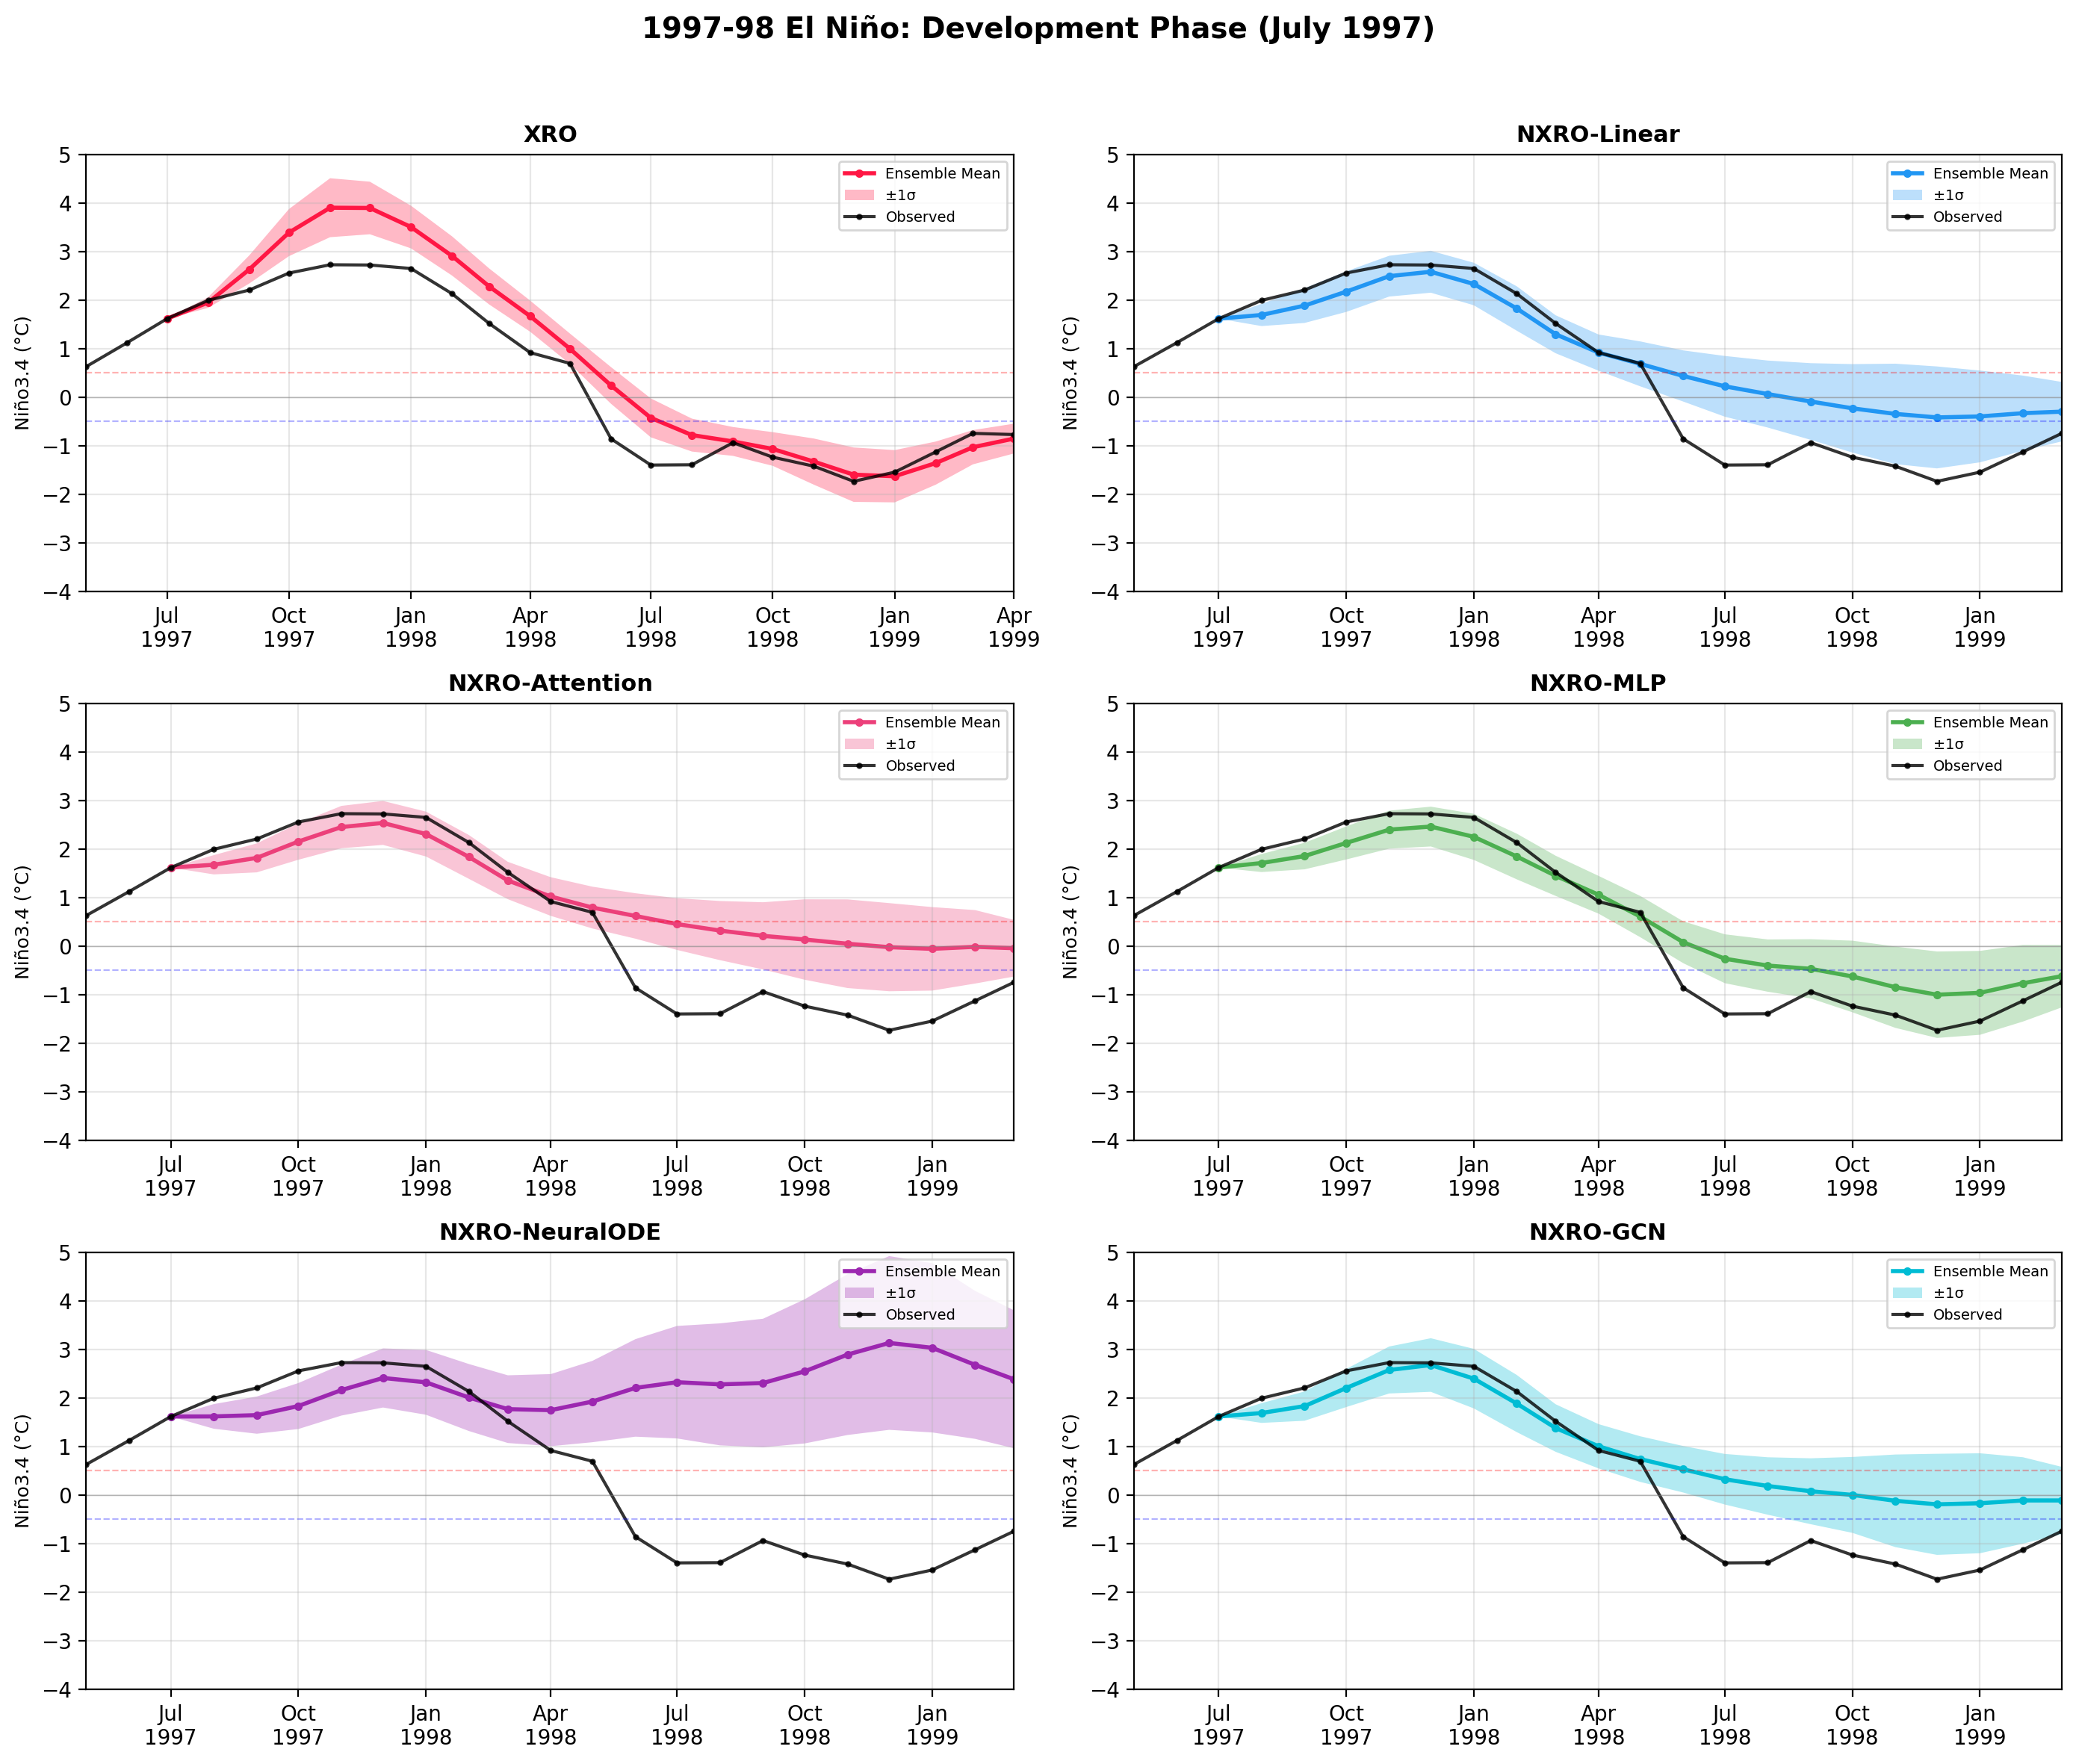
\includegraphics[width=0.8\columnwidth]{figures/elnino_1997_development.png}
  \caption{Stochastic forecast for ENSO development in 1997. Ensemble forecast comparison. Shaded regions show 10--90\% quantile ranges; solid lines show ensemble median; dots show observations.}
  \label{fig:1997_dev}
\end{figure}

\begin{figure}[t]
  \centering
  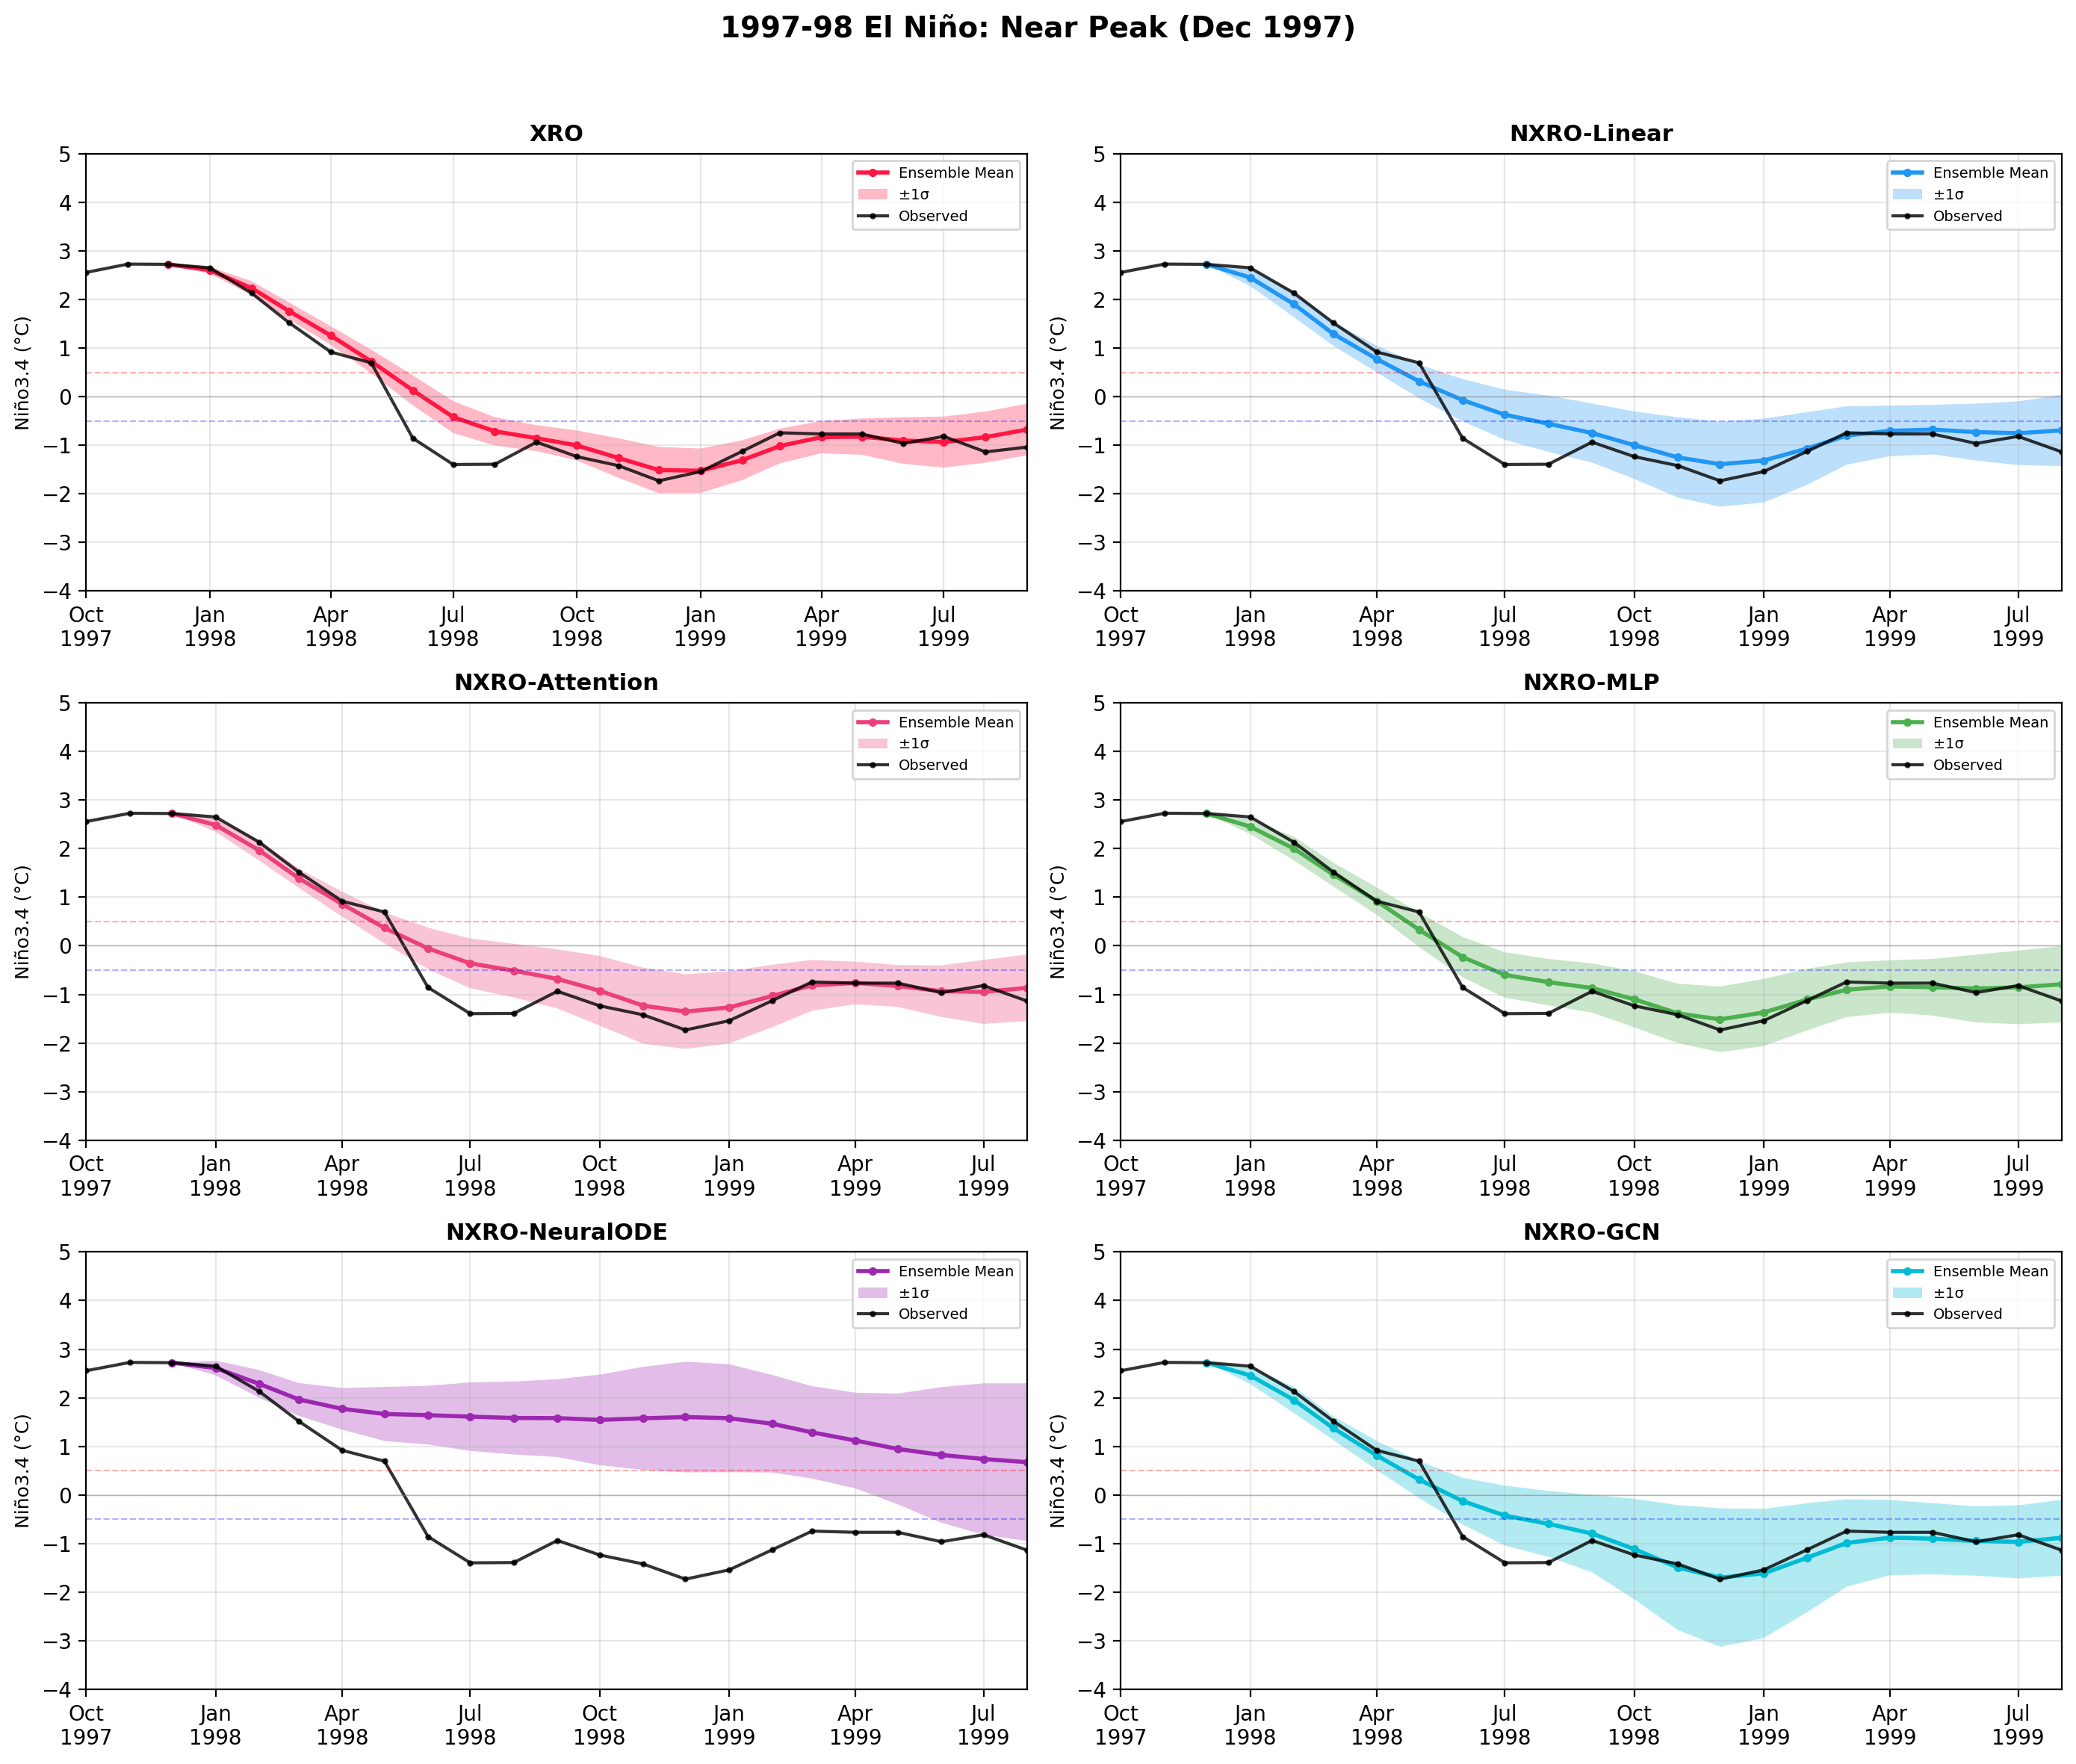
\includegraphics[width=\columnwidth]{figures/elnino_1997_peak.png}
  \caption{Stochastic forecast for ENSO peak in 1997. Ensemble forecast comparison. Shaded regions show 10--90\% quantile ranges; solid lines show ensemble median; dots show observations.}
  \label{fig:1997_peak}
\end{figure}


\begin{figure}[t]
  \centering
  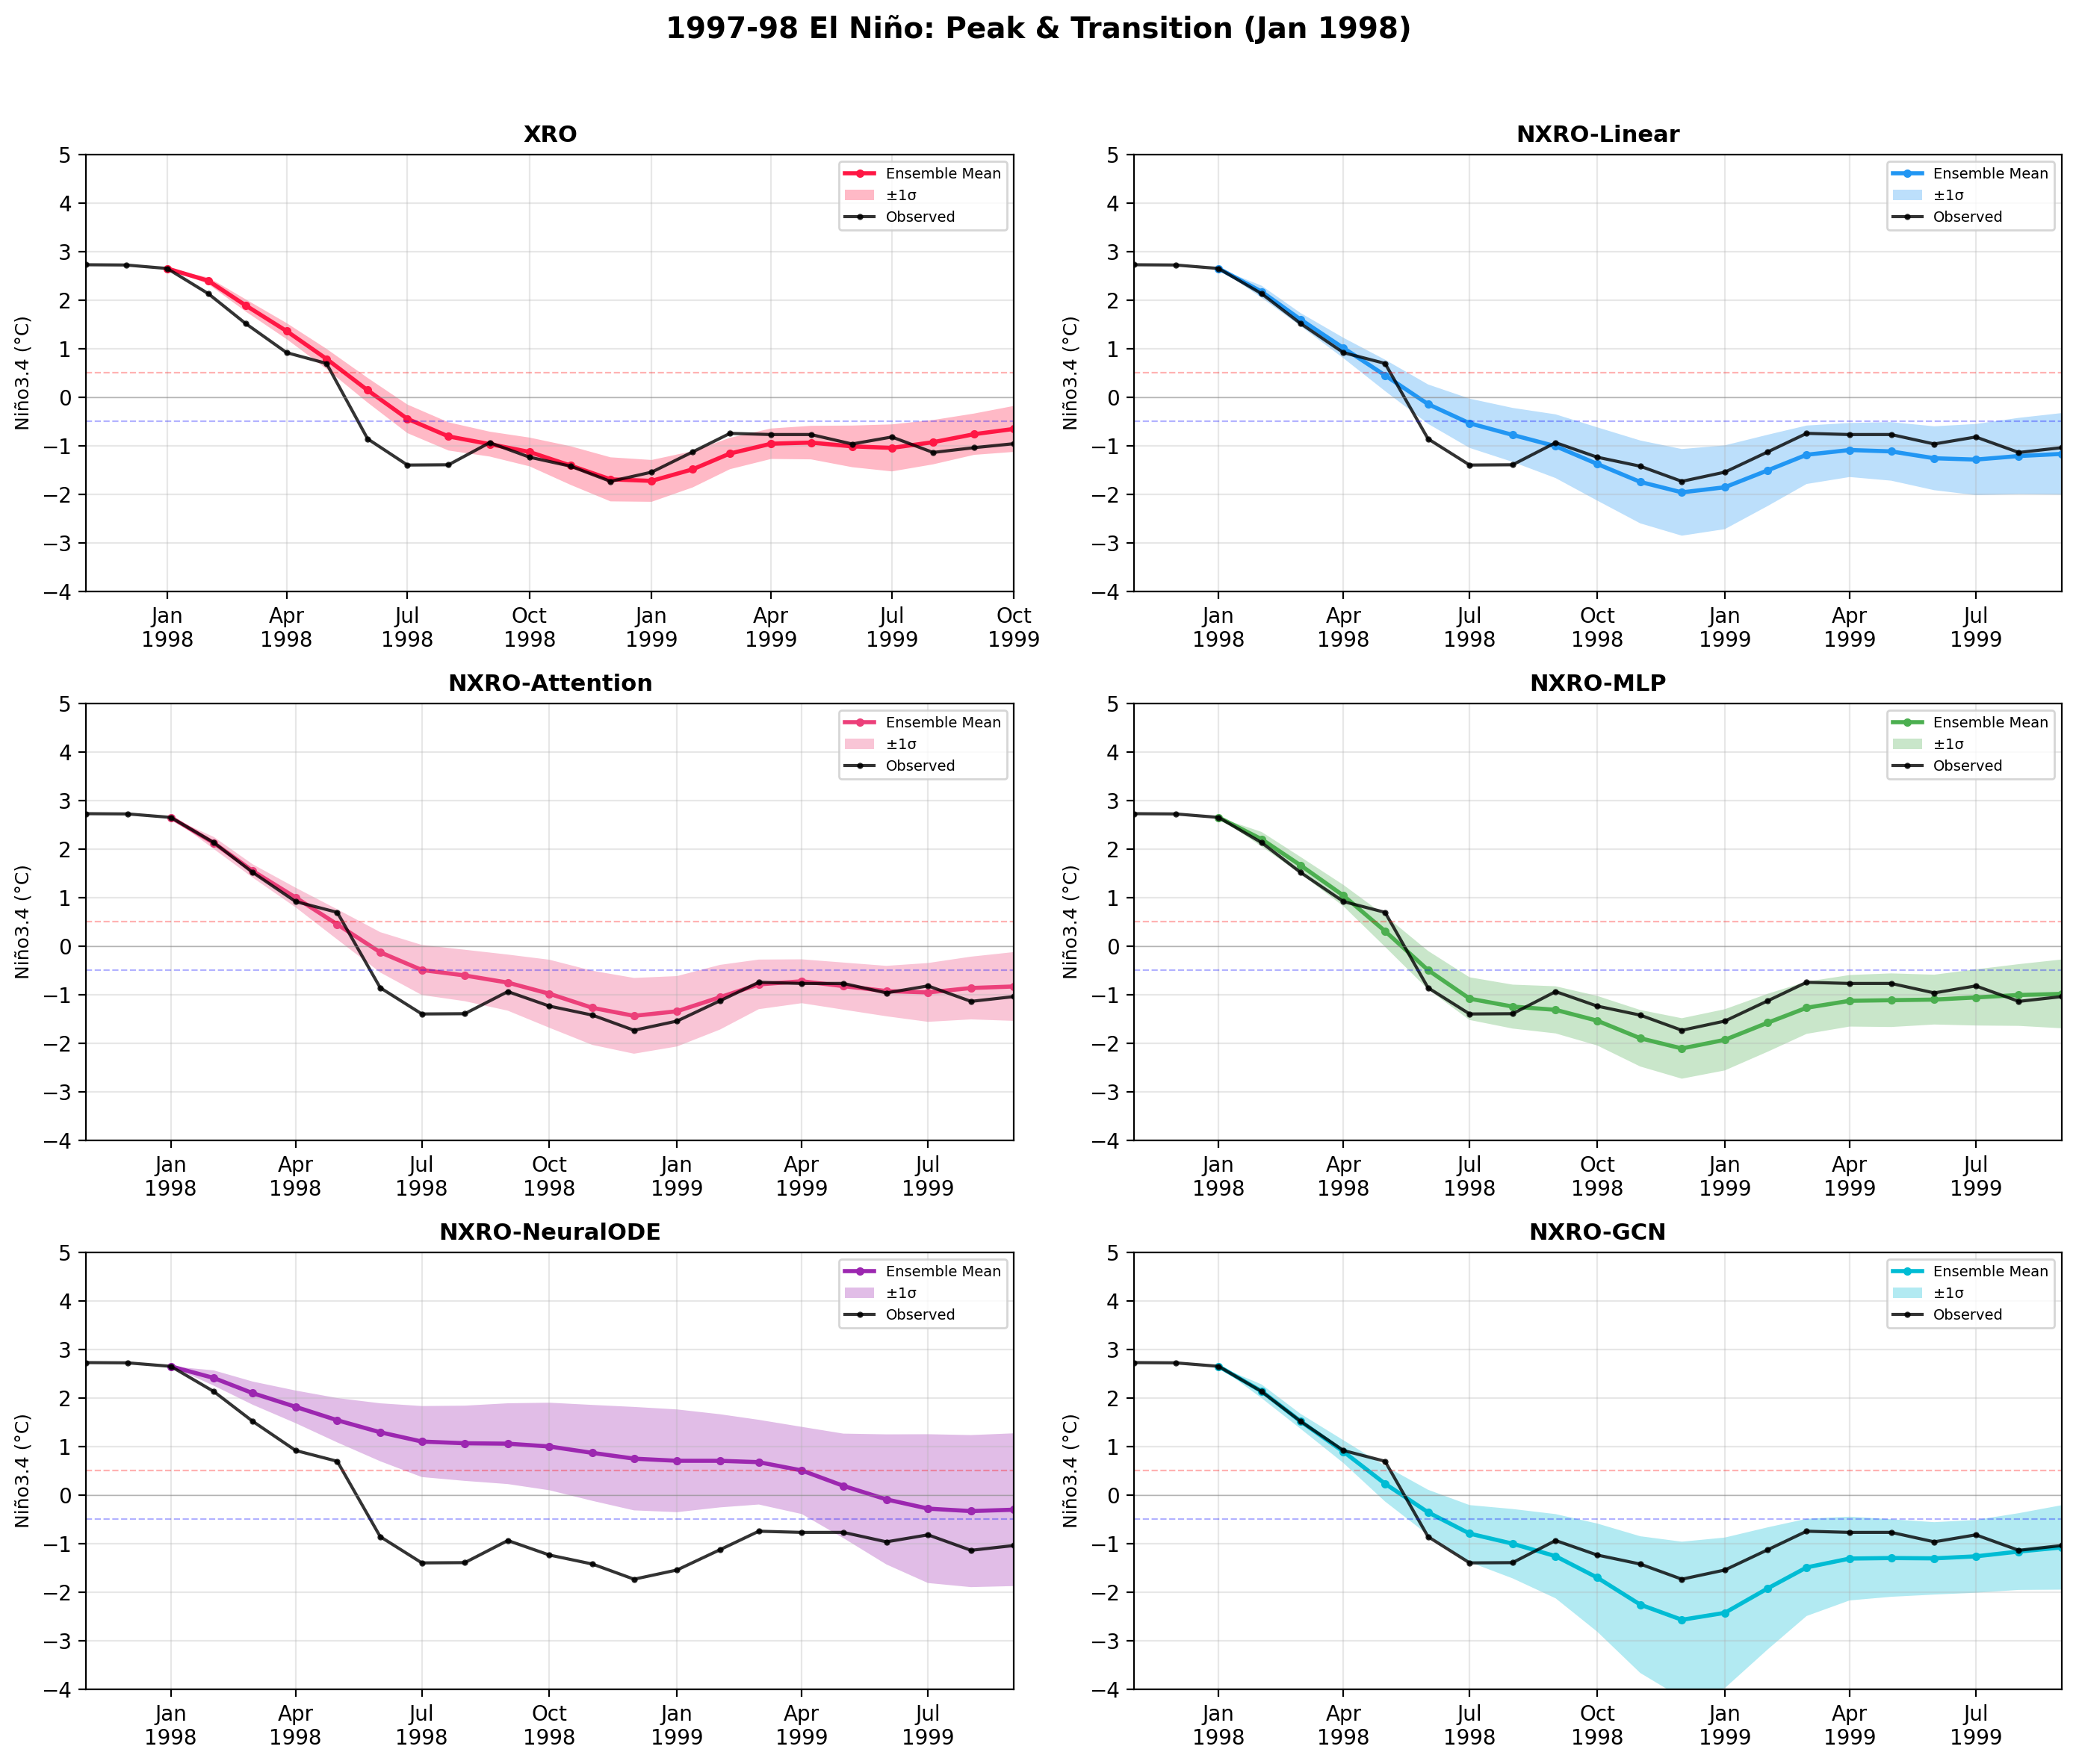
\includegraphics[width=\columnwidth]{figures/elnino_1998_transition.png}
  \caption{Stochastic forecast for ENSO transition in 1998. Ensemble forecast comparison. Shaded regions show 10--90\% quantile ranges; solid lines show ensemble median; dots show observations.}
  \label{fig:1998_trans}
\end{figure}

\begin{figure}[t]
  \centering
  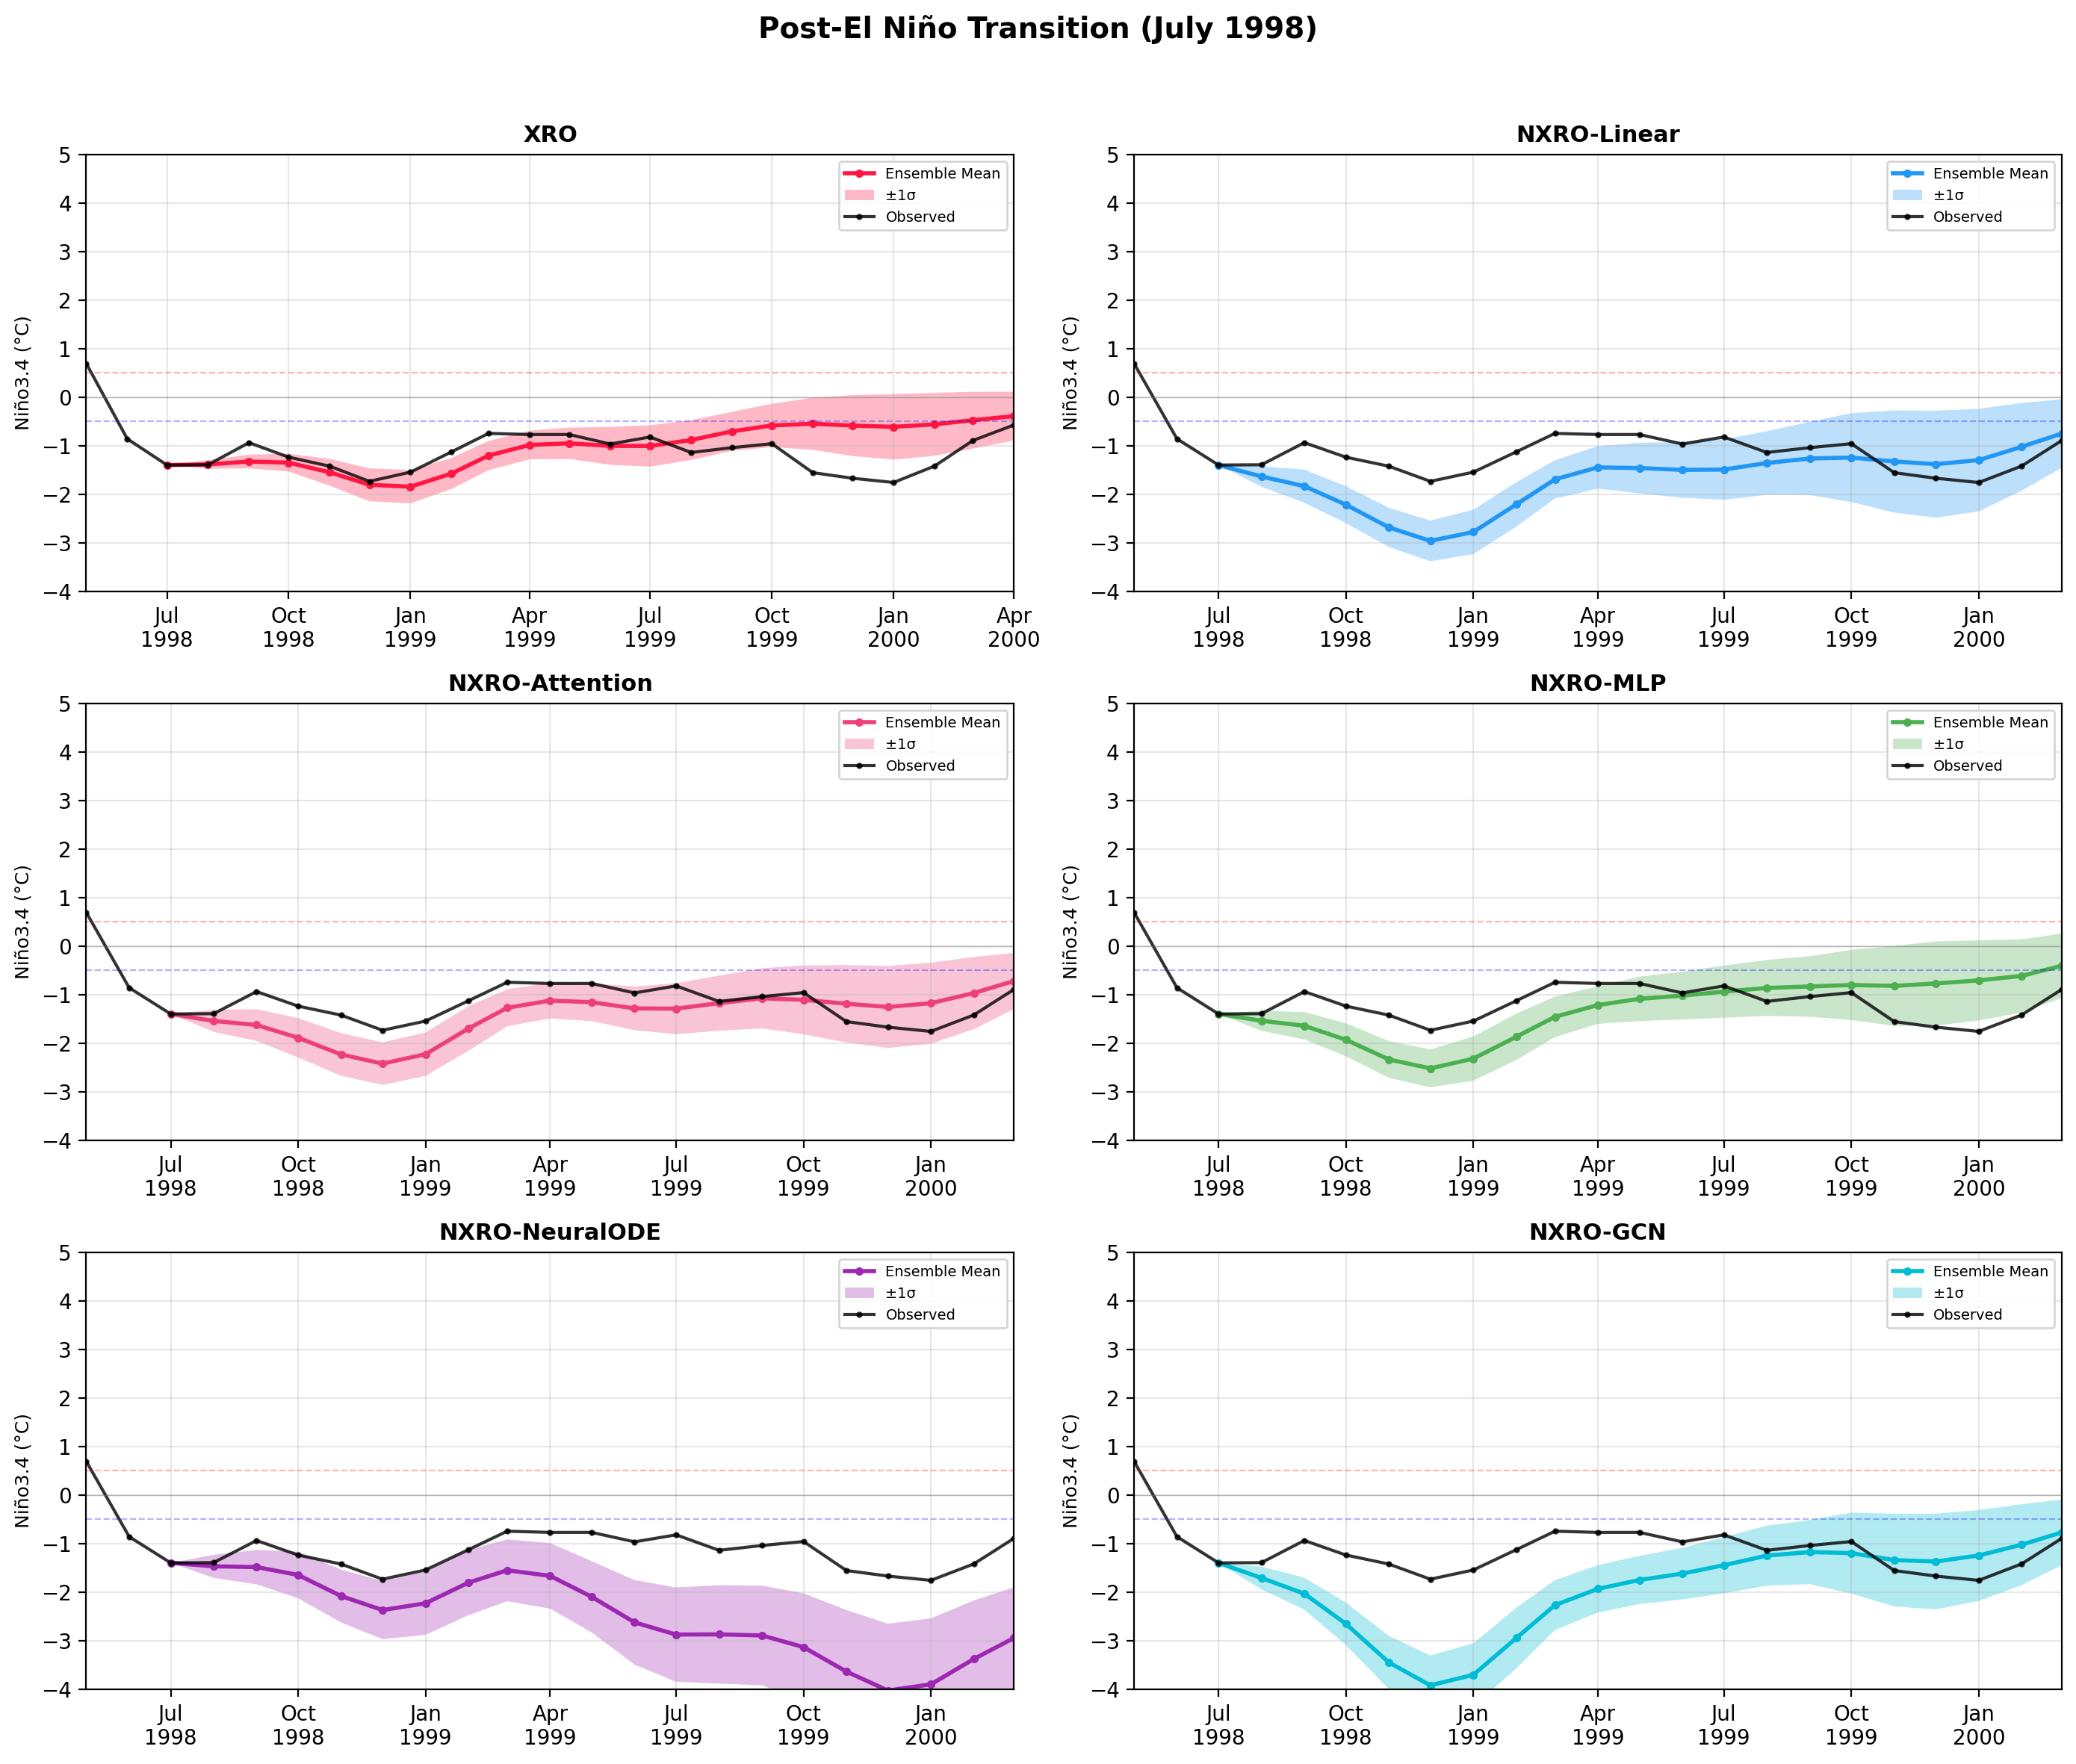
\includegraphics[width=\columnwidth]{figures/transition_1998_summer.png}
  \caption{Stochastic forecast for ENSO summer in 1998. Ensemble forecast comparison. Shaded regions show 10--90\% quantile ranges; solid lines show ensemble median; dots show observations.}
  \label{fig:1998_summer}
\end{figure}

% -------------------- Spring barrier (1997 / 1998) --------------------
\begin{figure}[t]
  \centering
  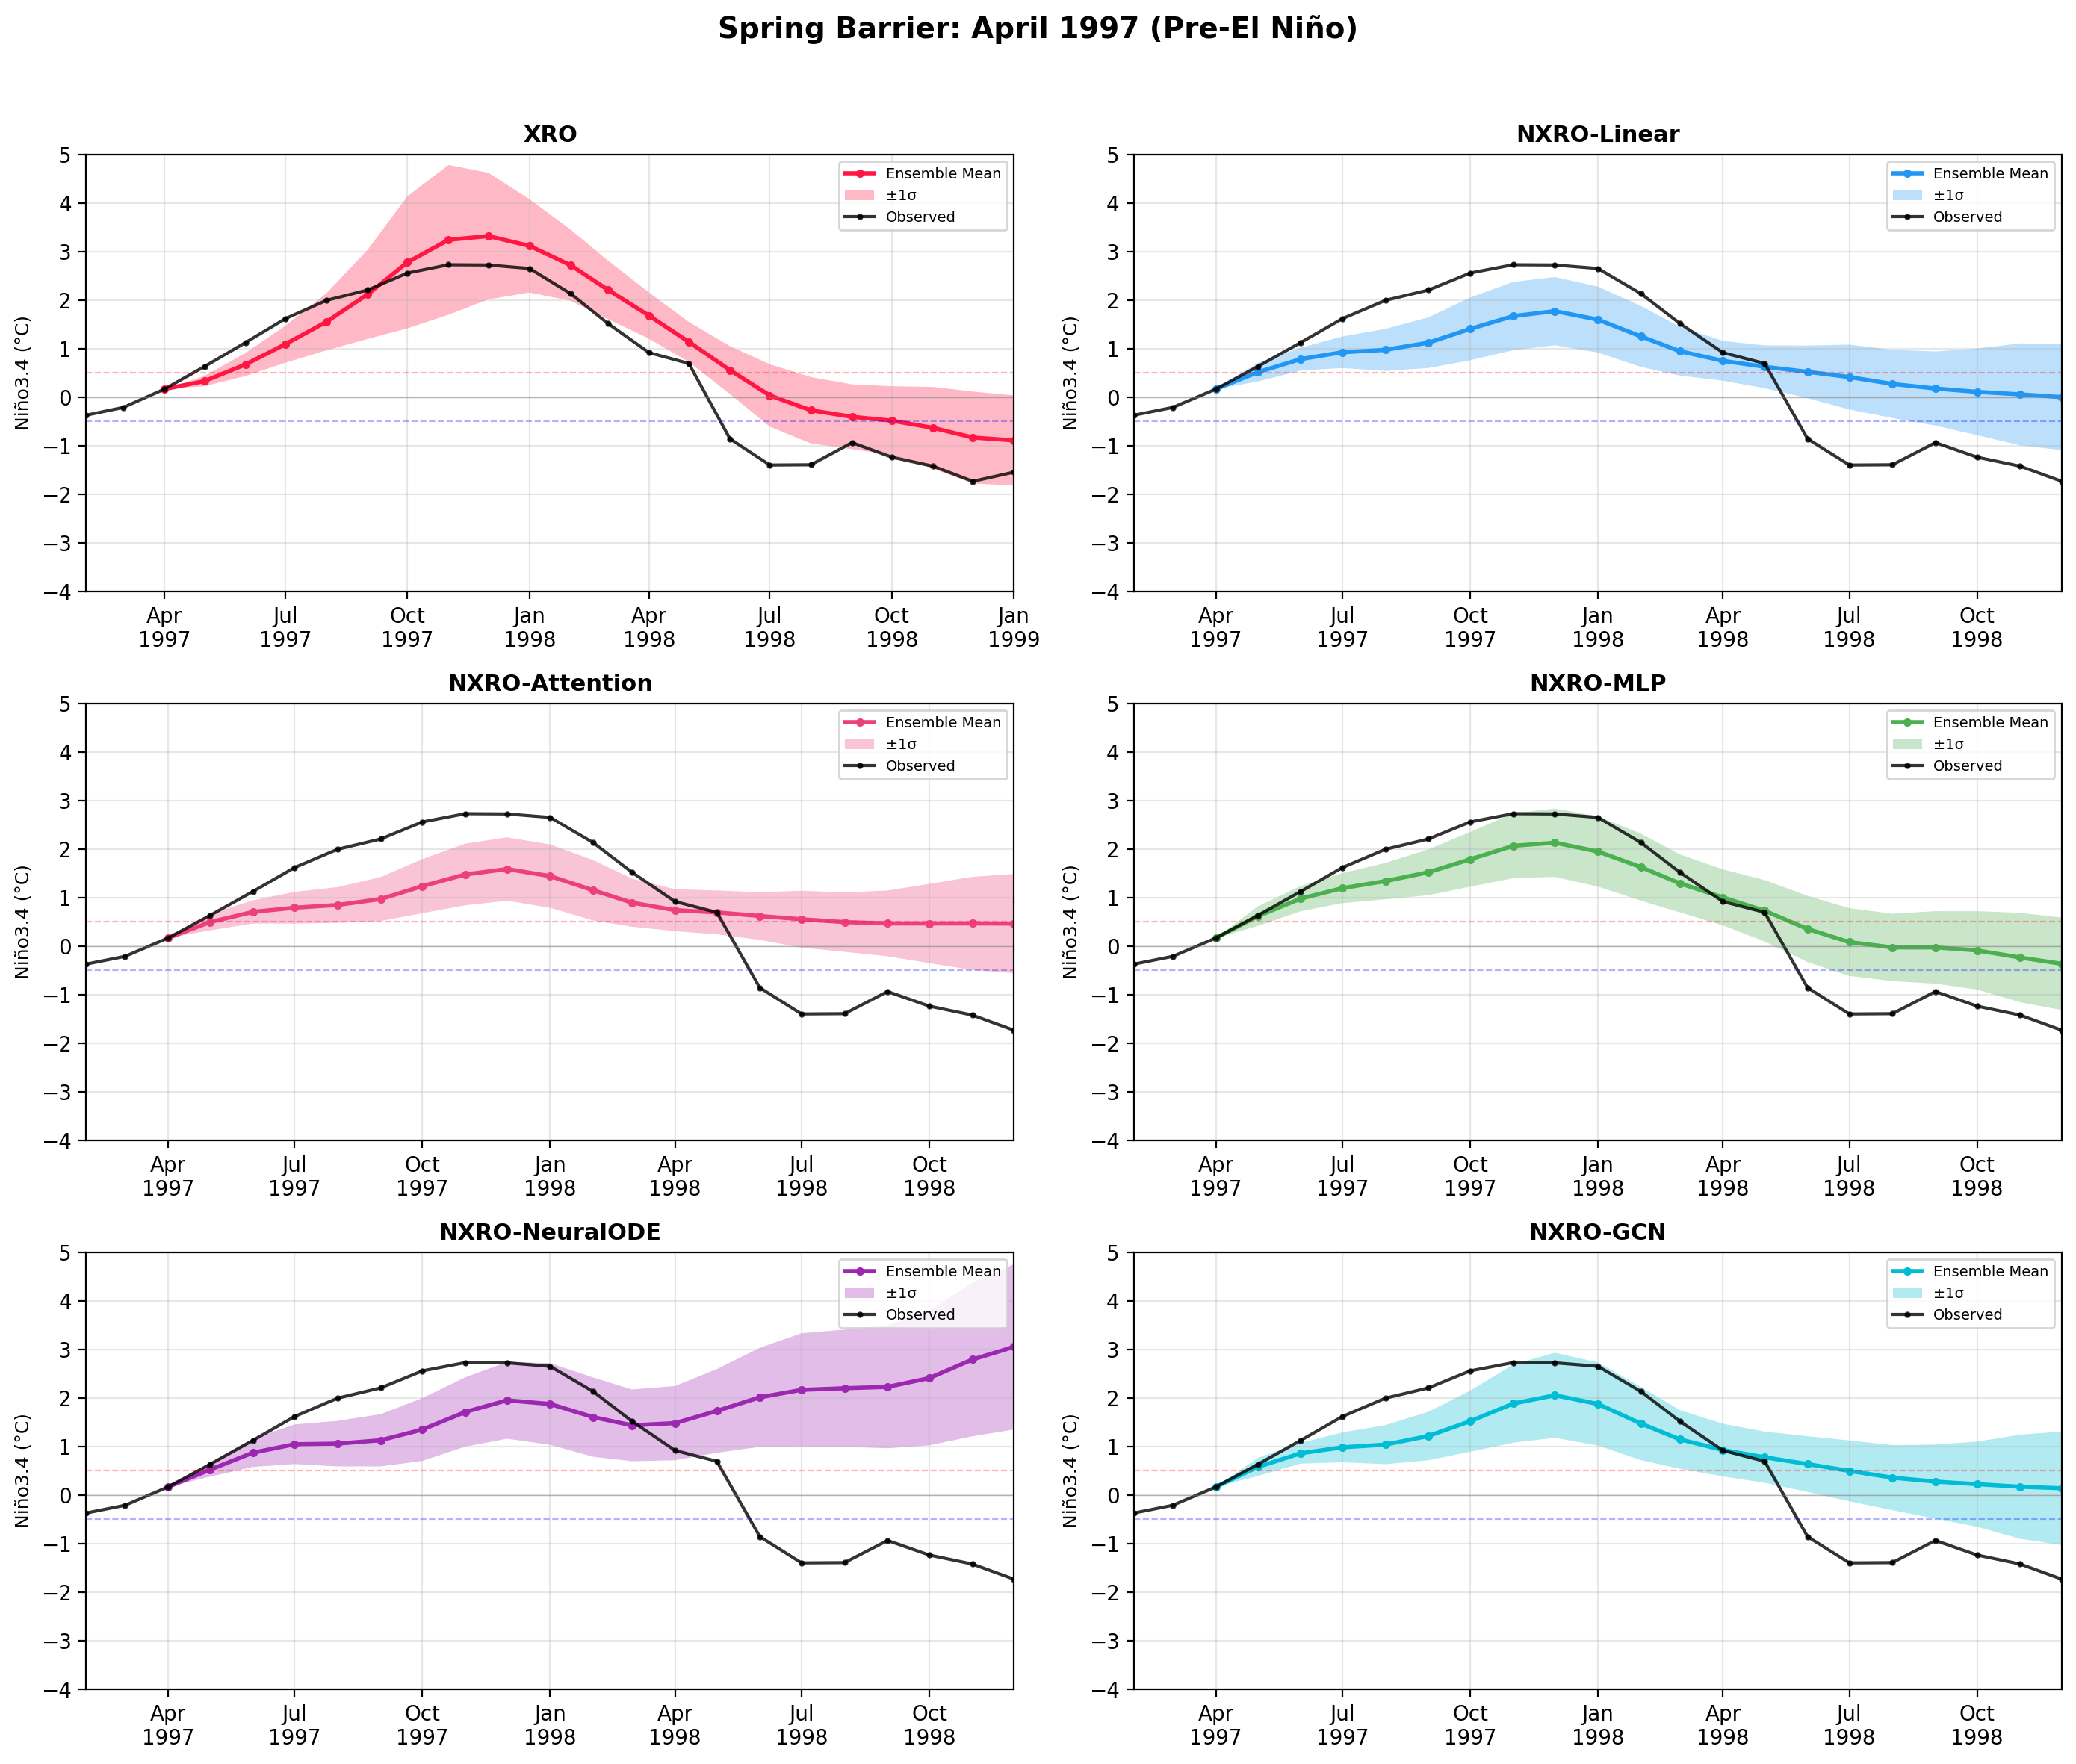
\includegraphics[width=\columnwidth]{figures/spring_barrier_1997.png}
  \caption{Stochastic forecast during spring barrier in 1997. Ensemble forecast comparison. Shaded regions show 10--90\% quantile ranges; solid lines show ensemble median.}
  \label{fig:1997_barrier}
\end{figure}

\begin{figure}[t]
  \centering
  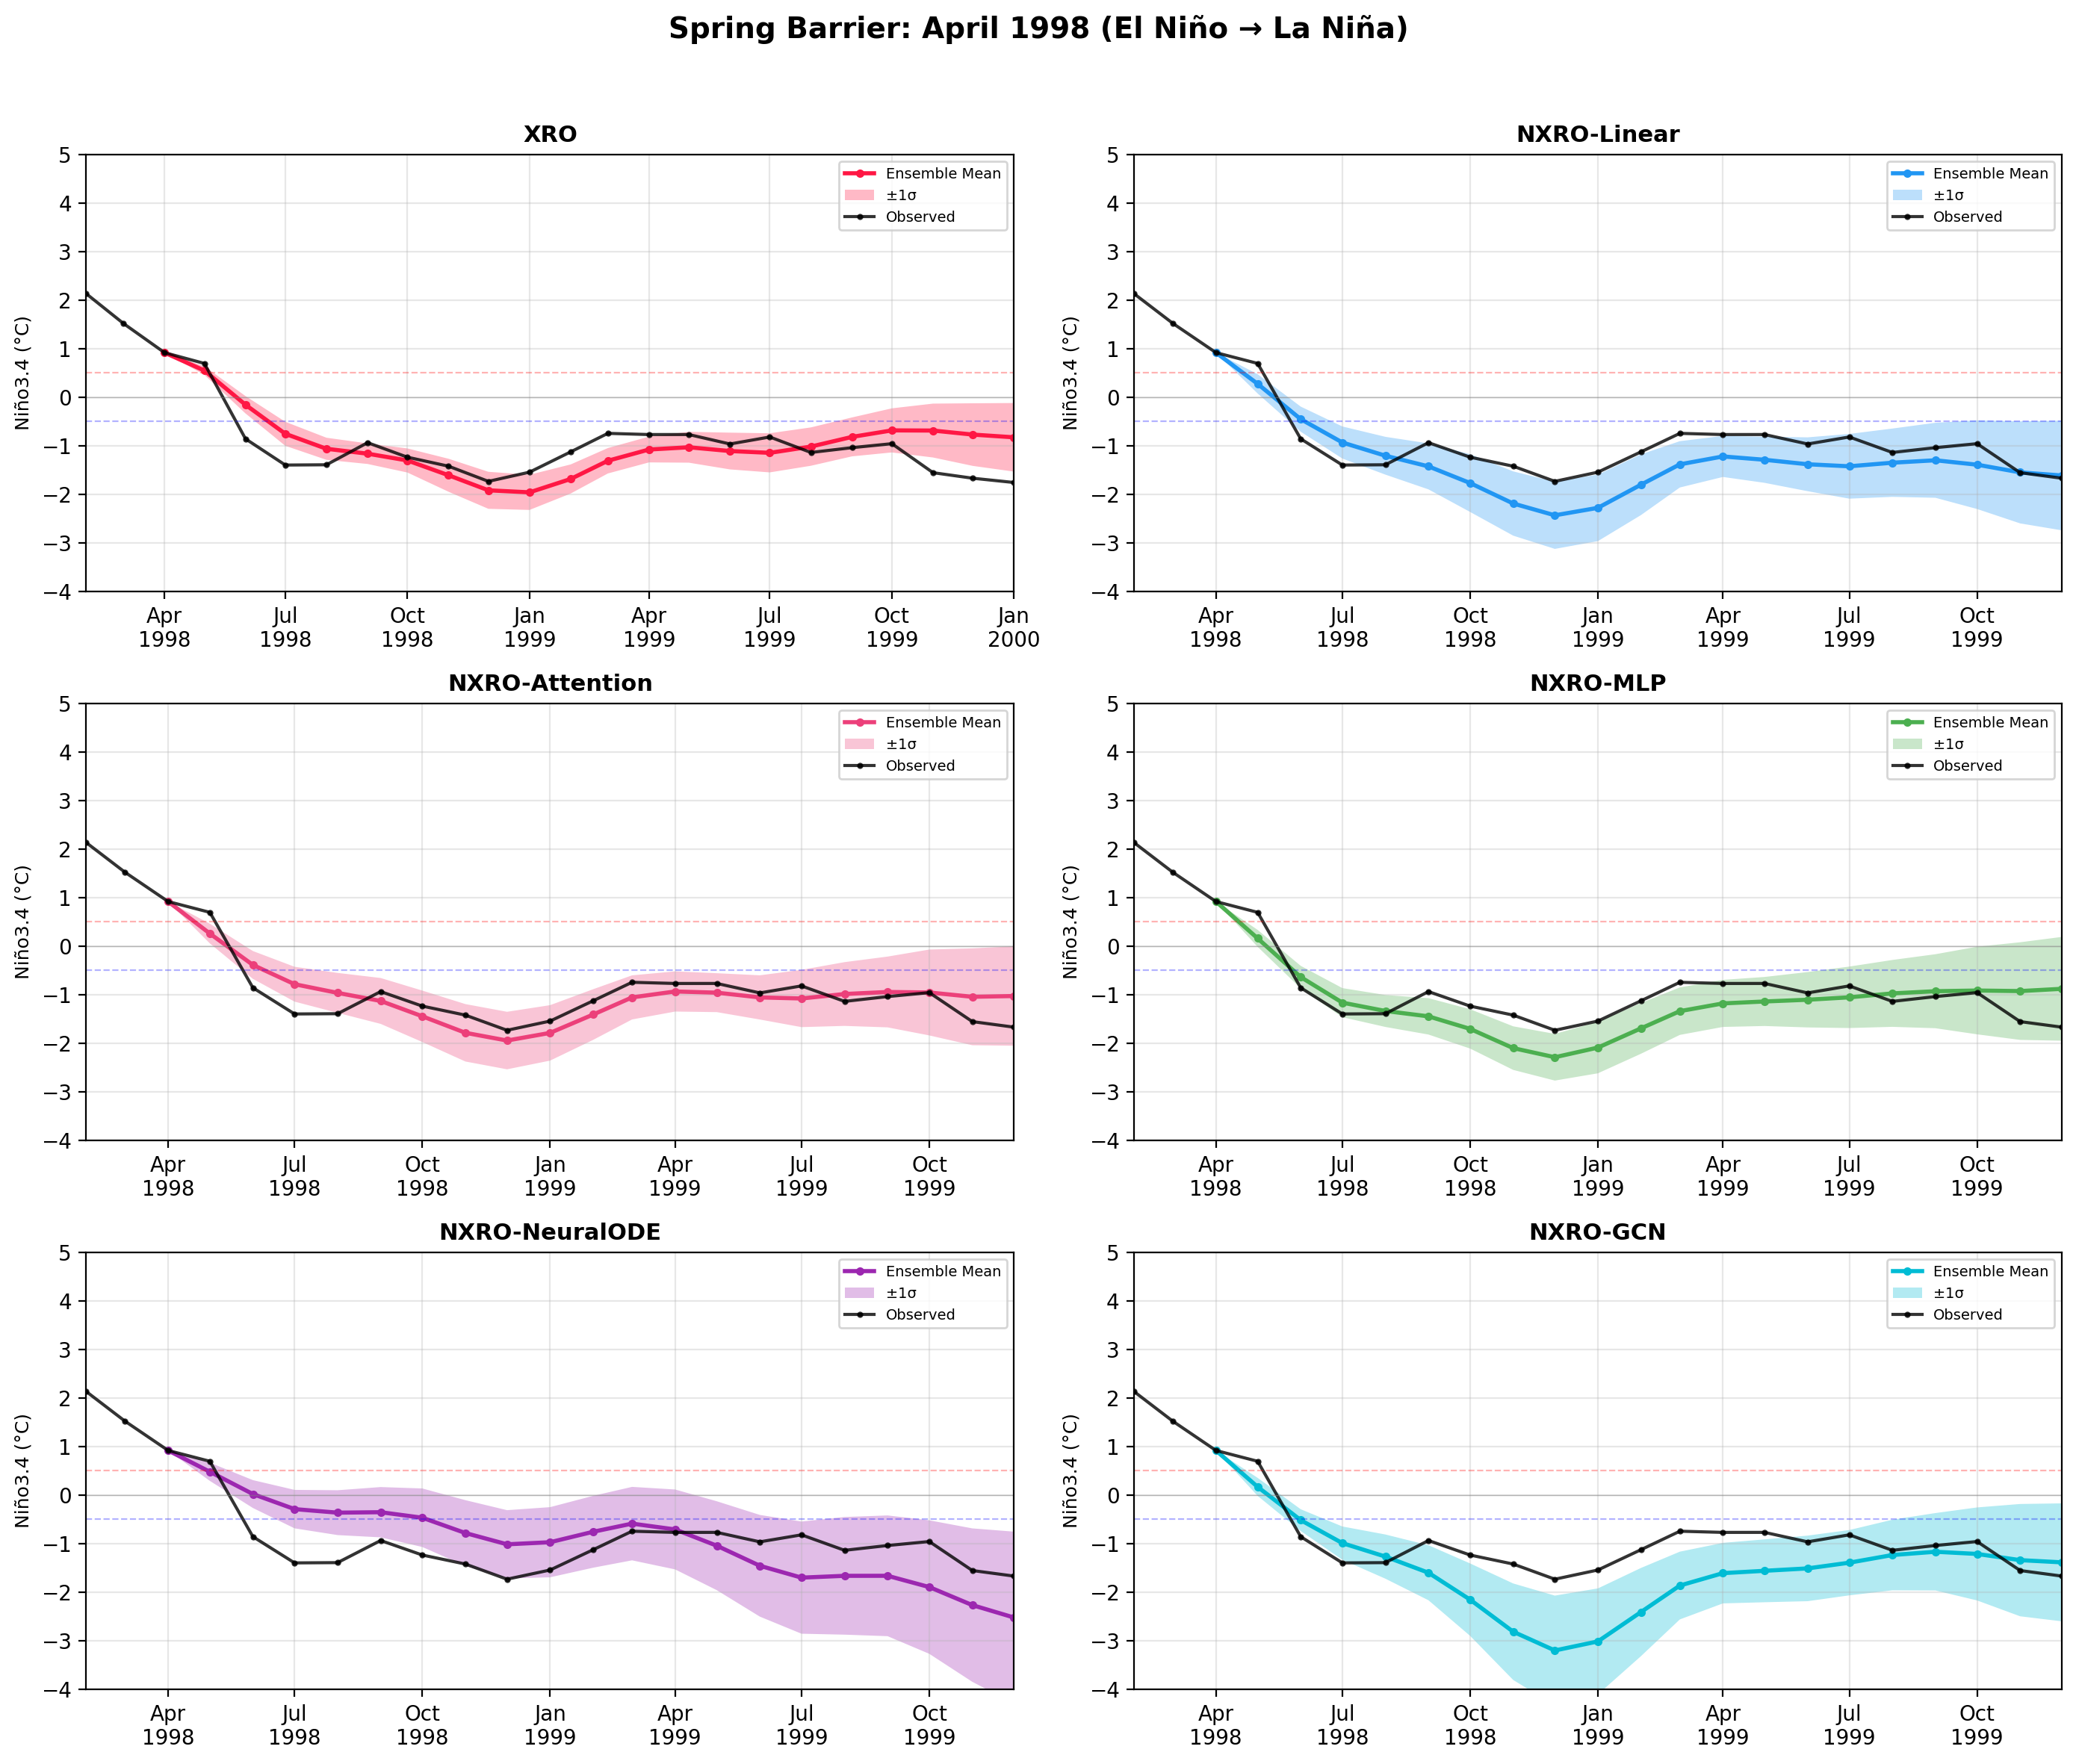
\includegraphics[width=\columnwidth]{figures/spring_barrier_1998.png}
  \caption{Stochastic forecast during spring barrier in 1998. Ensemble forecast comparison. Shaded regions show 10--90\% quantile ranges; solid lines show ensemble median.}
  \label{fig:1998_barrier}
\end{figure}

% -------------------- La Nina (2011 peak / 2010 development) --------------------
\begin{figure}[t]
  \centering
  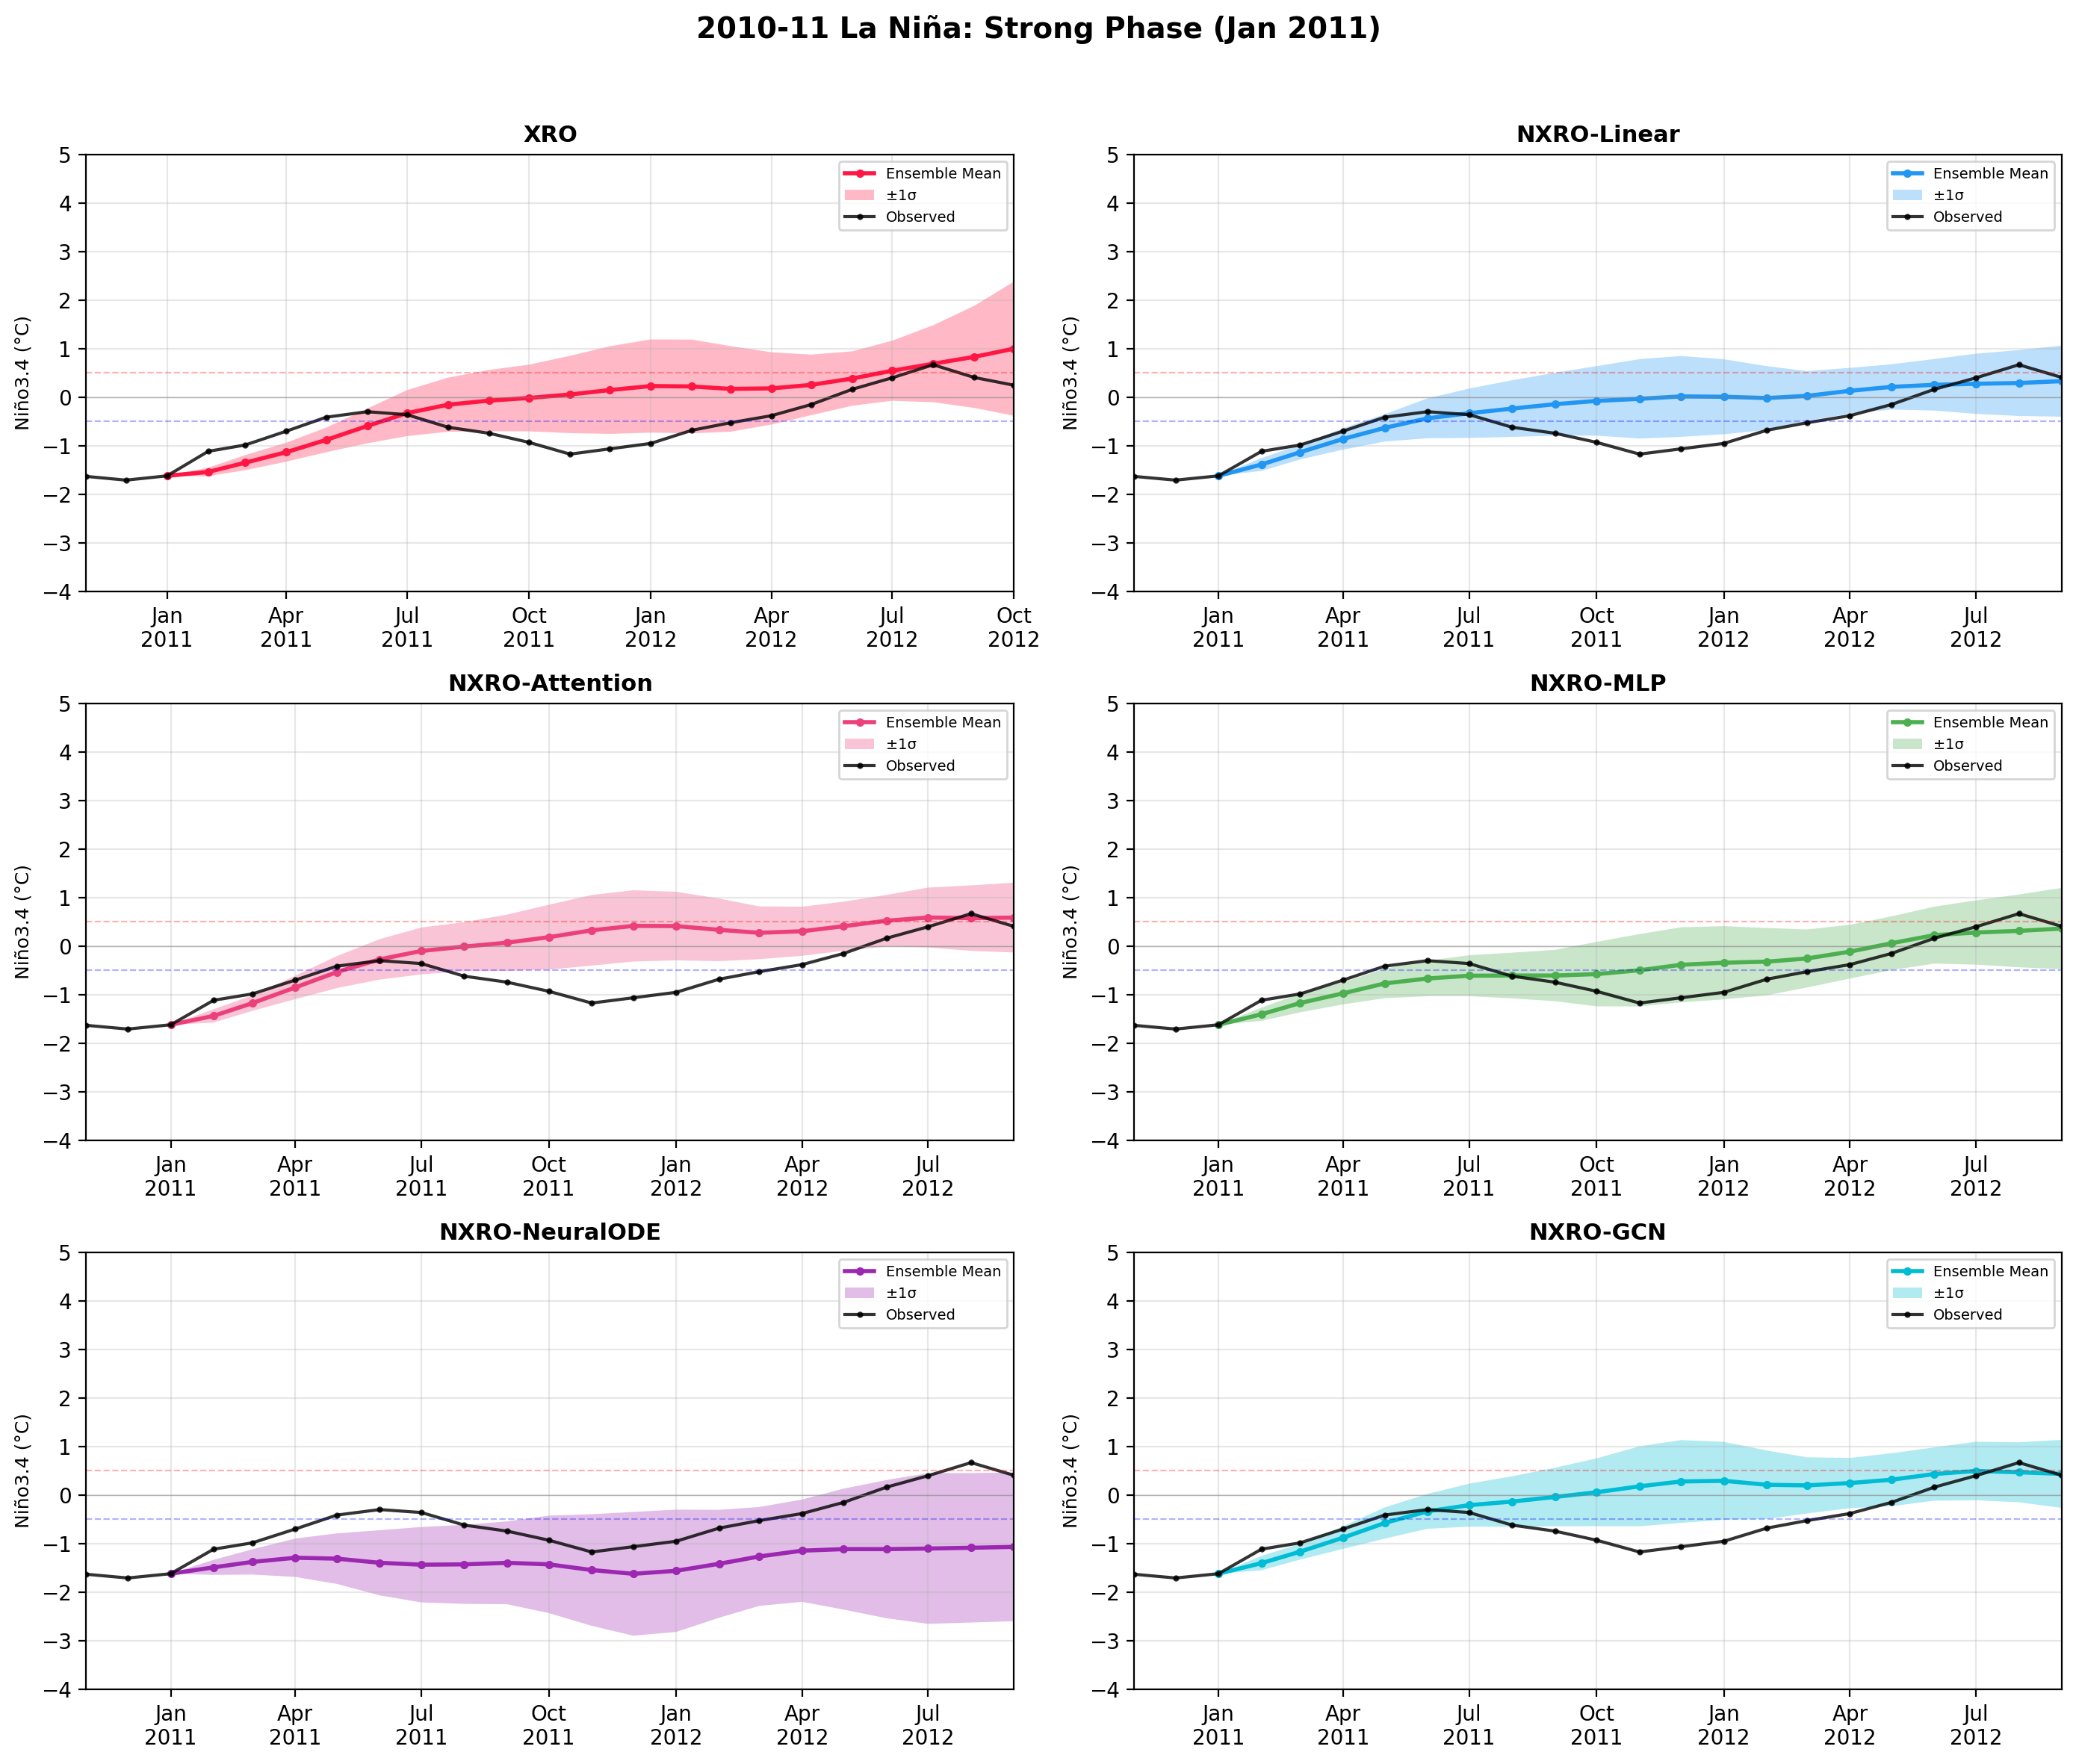
\includegraphics[width=\columnwidth]{figures/lanina_2011_peak.png}
  \caption{Stochastic forecast for the 2011 La Ni\~na peak. Ensemble forecast comparison.}
  \label{fig:2011_lanina}
\end{figure}

\begin{figure}[t]
  \centering
  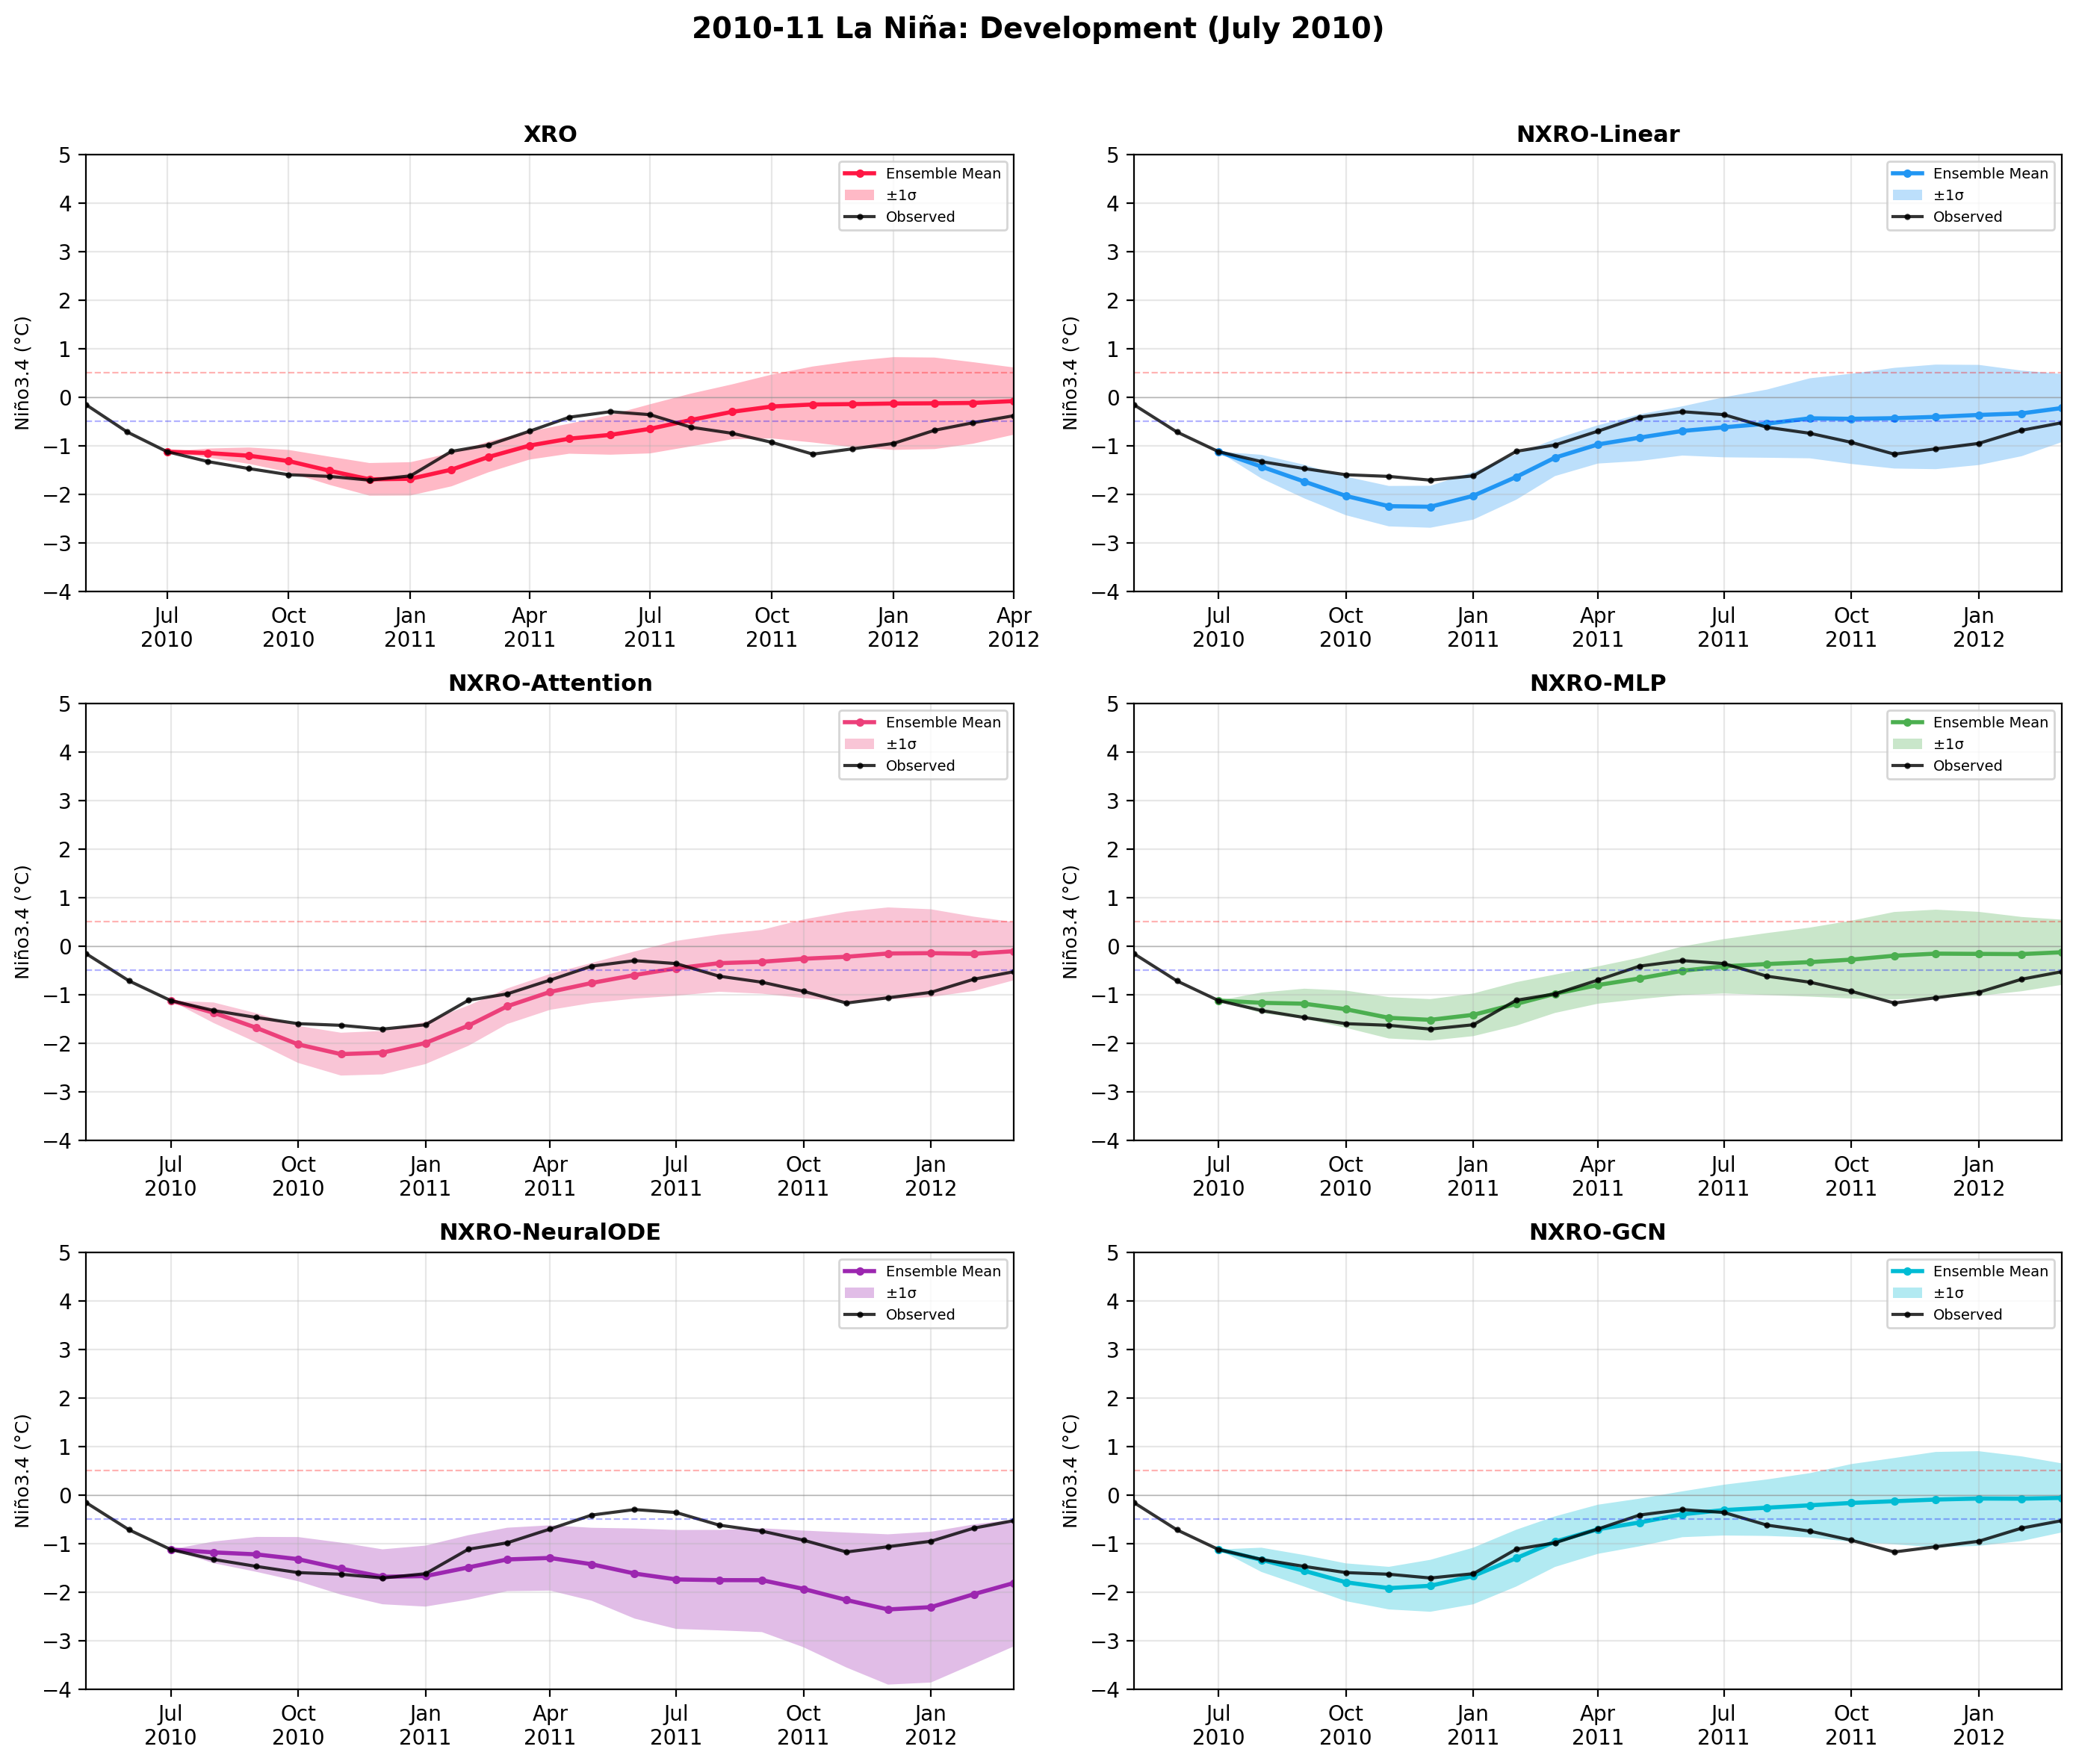
\includegraphics[width=\columnwidth]{figures/lanina_2010_dev.png}
  \caption{Stochastic forecast for 2010 La Ni\~na development. Ensemble forecast comparison.}
  \label{fig:2010_lanina}
\end{figure}


% \input{sections/D-Appendix}

\end{document}
